\documentclass[11pt, english]{article}
	\usepackage{geometry}
 		\geometry{
 			a4paper,total={210mm,297mm},
 			tmargin=40mm,
			bmargin=40mm,
			lmargin=32mm,
			rmargin=32mm,
 		}

	\usepackage{fancyhdr}
	\usepackage{lipsum}
		\pagestyle{fancy}
		\fancyhf{} 
		\fancyhead[L]{\leftmark}
		\fancyhead[R]{\thepage}
		\fancyfoot[C]{\thepage}
		\renewcommand{\headrulewidth}{0.5pt}

	\usepackage{tocloft}
		
		\renewcommand{\cfttoctitlefont}{\fontsize{18}{16}\scshape}
		\renewcommand{\cftlottitlefont}{\fontsize{18}{16}\scshape}
		\renewcommand{\cftloftitlefont}{\fontsize{18}{16}\scshape}

		\renewcommand{\cftsecfont}{\scshape}
		\renewcommand{\cftsubsecfont}{\scshape}
		\renewcommand{\cftsubsubsecfont}{\scshape}
		\renewcommand{\cftparafont}{\scshape}

	\usepackage{abstract}
		\renewcommand{\abstractnamefont}{\fontsize{11}{0}\scshape}

	\renewcommand{\thesection}{\arabic{section}}
	\renewcommand{\thesubsection}{\thesection.\arabic{subsection}}
	\renewcommand{\thesubsubsection}{\thesubsection.\arabic{subsubsection}}
	\renewcommand{\theparagraph}{\thesubsubsection.\arabic{paragraph}}

	\usepackage{titlesec}

		\titleformat{\section}
			{\fontsize{18}{16}\scshape}{\thesection}{0.5em}{}

		\titleformat{\subsection}
			{\fontsize{14}{16}\scshape}{\thesubsection}{1em}{}

		\titleformat{\subsubsection}
			{\fontsize{11}{16}\scshape}{\thesubsubsection}{1em}{}

		\titleformat{\paragraph}
			{\fontsize{11}{16}\scshape}{\theparagraph}{1em}{}

	\usepackage{hyperref} 
		\hypersetup{          
        		colorlinks=true,        
        		linkcolor=black,  
        		filecolor=magenta,
        		urlcolor=cyan,
        		}

	\usepackage{caption}
		\captionsetup[table]{labelfont=sc,textfont=sc,font=small,skip=8pt}
		\captionsetup[figure]{labelfont=sc,textfont=sc,font=small,skip=8pt}
	\usepackage{subcaption}
		\captionsetup[subtable]{justification=raggedright,labelfont=sc,textfont=sc,font=small,skip=8pt,labelformat=parens,labelsep=space}
		\captionsetup[subfigure]{justification=raggedright,labelfont=sc,textfont=sc,font=small,skip=8pt,labelformat=parens,labelsep=space}

	\usepackage{float}

		\renewcommand{\thetable}
			{\thesection.\arabic{table}}

		\renewcommand{\thefigure}
                 	{\thesection.\arabic{figure}}
         	\renewcommand{\thesubfigure}
                	{\roman{subfigure}}

	\setlength{\parindent}{0pt}

	\renewcommand{\baselinestretch}{1.25}
	\usepackage{setspace}

	\newcommand{\HRule}[1]{\rule{\linewidth}{#1}}
		\setcounter{tocdepth}{5}
		\setcounter{secnumdepth}{5}

	\usepackage{longtable}
	\usepackage{multicol}
	\usepackage{multirow}

	\usepackage{amsmath}
	\usepackage{amssymb}

	\usepackage{graphicx}
	\graphicspath{{./Photos/}}

	\usepackage{tikz}
		\usetikzlibrary{trees,arrows,topaths}

	\usepackage[utf8]{inputenc}
	\usepackage[T1]{fontenc}

	\usepackage{lscape}
	\usepackage{colortbl}

	\usepackage{tipa}

	\usepackage{babel}

        \usepackage{color}
                \definecolor{lightgrey}{rgb}{0.9,0.9,0.9}
                \definecolor{darkgrey}{rgb}{0.4,0.4,0.4}
                \definecolor{purple}{rgb}{0.65,0.12,0.82}

        \usepackage{listings}

		\lstdefinelanguage{JavaScript}{
			keywords={typeof, new, true, false, catch, function, return, null, catch, switch, const, var, let, for, if, in, while, do, else, case, break},
			keywordstyle=\color{blue}\bfseries,
			ndkeywords={class, export, boolean, throw, implements, import, this},
			ndkeywordstyle=\color{darkgrey}\bfseries,
			identifierstyle=\color{black},
			sensitive=false,
			comment=[l]{//},
			morecomment=[s]{/*}{*/},
			commentstyle=\color{purple}\ttfamily,
			stringstyle=\color{red}\ttfamily,
			morestring=[b]',
			morestring=[b]"
		}

		\lstset{
			language=JavaScript,
			backgroundcolor=\color{lightgrey},
			extendedchars=true,
			basicstyle=\scriptsize\ttfamily,
			showstringspaces=false,
			showspaces=false,
			numbers=left,
			numberstyle=\footnotesize,
			numbersep=9pt,
			tabsize=2,
			breaklines=false,
			showtabs=false,
			captionpos=b
		}

	\usepackage{dirtree}

\begin{document}

% Title Page

\pagenumbering{gobble}

	\title{
		\HRule{0.5pt}\\ [-0.9cm]
                \HRule{0.5pt}\\ [0.4cm]
                \huge\textsc{CS958 Project}\\
                \Large\textsc{Coursework Assignment}\\ [0.25cm]
		\HRule{0.5pt}\\ [-0.725cm]
                \HRule{0.5pt}
                }
	\author{
		\begin{tabular}{c}
			\textit{Original Screenplay By}\\
			\textsc{Lewis W. Britton, L.W.B.}\\
			\hline
			\hline
		\end{tabular}\\
                \textsc{202194412}\\
                \textsc{University of Strathclyde}\\
		\textit{Glasgow City, Scotland}
                }
	\date{}
	\maketitle

        \begin{center}
		\huge{\textsc{Burning Roots}}
        \end{center}

        \vspace{\fill}

	\begin{center}
	\begin{tabular}{c}
		\textit{Written \& Directed By}\\ \textsc{John Hughes}\\
		\hline
		\hline
		\textit{Executive Producer}\\ \textsc{Michael Mann}\\
		\hline
		\hline
		\textit{Created By}\\ \textsc{Anthony Yerkovich}\\
		\hline
		\hline
		\textit{Music Composed \& Performed By}\\ \textsc{Jan Hammer}\\
	\end{tabular}
	\end{center}

	\begin{center}
		\fbox{\textsc{... Words}}
	\end{center}

	\begin{center}
        	\textsc{Dissertation Submitted in Partial Fulfilment of the Requirements for the Degree of Master of Science Software Development at the University of Strathclyde}
	\end{center}

	\begin{center}
		\textsc{Academic Year 2021/2022}
	\end{center}

\newpage

\pagenumbering{roman}

	\begin{abstract}
		This piece extensively details and provides context to all components of the system I've developed for this project: \textit{Burning Roots}. The system explores the context of the system, being the Scottish highlands; it's landmasses and their routes, with additional components such as ability factors, equipment (`gear') factors and the contribution of weather. The system is written in HTML, CSS and JavaScript; uses JSON data store for high-level querying; implements GPX files using the GPX-to-GeoJSON method; uses user-specific location services through the Geolocation API; accesses weather data using the OpenWeather API; and present the user with an interactive map, based on these factors, using the Ordnance Survey API and Leaflet. Post-completion of the system, this piece details all elements of the software development process which have been practiced, including: requirement gathering; development environments; the user interface logic and design; data storage and use; continuous prototyping; continuous test-driven development; user testing; and accessibility and usability factors. It finds that opportunities taken, with reference to the selected languages, APIs and libraries, etc., efficient routes are selected and client criteria are successfully met, although there remains adequate room for expansion and improvement given the nature of the scripting; how functions are written and interlink, etc.
	\end{abstract}

	\textsc{Index terms}: web application, website, site, system, geography, hiking, landmasses, routes, ability, equipment, weather forecasting, location services, HTML, CSS, JavaScript, JSON, GPX, Geolocation API, Ordnance Survey API, OpenWeather API, Leaflet, Mapbox GL-JS, graphic design, photo manipulation, software development, client requirements gathering, development environments, user interface, data, prototyping, test-driven development, user testing, accessibility, usability

\newpage
% Declaration

	\section*{Declaration \& Information}

	This dissertation is submitted in partial fulfilment of the requirements for the degree of Master of Science Software Development at the University of Strathclyde. It accords with the University’s regulations for the programme as detailed in the University Calendar.

	\begin{center}
		\small
	\begin{tabular}{p{5.45cm}|p{5.45cm}}
		\textsc{Mail To:} wi.lbritton@yahoo.com & \textsc{Telephone:} 07415 212 ***\\
		\textsc{Website:} \href{http://lewisbritton.com}{lewisbritton.com} & \textsc{GitHub:} \href{https://github.com/FedeRog1977}{FedeRog1977}\\
	\end{tabular}
	\end{center}

	This document’s presentation reflects the use of {\LaTeX} typesetting (Figure B1), using Computer Modern Unicode (Figure B2). Unfortunately {\TeX}\ does not support the required selection of packages for this project, such as \texttt{tikz} and various code markup and math packages. Hence, PDFs are produced using the (PDF){\LaTeX}\ compiler, although (\textsc{Xe}){\LaTeX}\ could have been useful in places. Due to time constraints, I've not been able to master the fine art of GNU Troff, so transcriptions will not be blessed by the Groff-PostScript combo. Processes such as these help escape the inane formatting requirements of my institution. References are presented using \textsc{Bib}{\TeX}, favouring \textsl{oblique} over \textit{italic}, in-line with Donald E. Knuth’s preference (Knuth, 2020). The process is executed in command line using a newer version of Emperor Moolenaar's Vim (Moolenaar, 2020), neoVim, which is a very powerful editor that has many commands, too many to explain in a tutor such as this. It yields the `Full Vi Experience' (Vim Diesel, 2020). For maximum optical pleasure, such alike a photo of Lily Collins, the use of Zathura (not M$\mu$PDF!) is vigorously advised, with inversion (not sandwich). Ensure you have an appropriate \texttt{config}. Navigate this document using h($\leftarrow$), j($\downarrow$), k($\uparrow$), l($\rightarrow$), ensuring that the Caps-Lock, Super-Key `mod', or any other command key is not depressed.\\

	The Oxford Serial Comma is favoured throughout this text. Sentence structure focuses on pragmatics and syntax, disregarding bloat. Arguments are coherent, logical, definitive and straight-to-the-point. Nugatory Soylicon Cuckley soydev `theory' is ignored. If you're curious about any of the mathematical, operational, logical, etc., symbols or notation used in this report, a comprehensive {\LaTeX}-syntax-based symbolist is available \href{http://lewisbritton.com/Library.html/Writings/Symbol-List.pdf}{here}.\\
 
	The word count of this piece reflects content from section heading classes 1, 2, 3 and 4, paragraphs, and footnotes in \textit{Sections 1 $\rightarrow$ 7}. Word count excludes any pre/succeeding content from \textit{Abstract}, \textit{Declaration \& Information}, \textit{Acknowledgements}, \textit{Table of Contents}, \textit{List of Tables}, \textit{List of Figures}, \textit{Appendices}, and \textit{Bibliography}. It also excludes content from tables, table titles, figures, and figure titles.\\

	I declare that this document embodies the results of my own work and that it has been composed by myself. Following normal academic conventions, I have made due acknowledgement of the work of others.\\

	Signed:\\ 

	Date:

\newpage
% Acknowledgements

	\section*{Acknowledgements}

	I would like to thank my dissertation supervisor, Alasdair Lambert, for his appropriate approach towards meetings and progress reporting. With support on a by-student basis, it is encouraging to be self-disciplined, organised, structured and punctual to one's own degree. This closely relates to my own practiced work ethic and idea of the ASAP standard. Again, no bloat such as formal planning practices or void meeting time.\\

	I would like to give credit for the computational aspect of this study to one of my biggest inspirations, \href{http://lewisbritton.com/Blog/Founding-Fathers.html}{John ``The ``J-Money'' Tzar'' Kelly}. He inspired my love for everything from arrays (of hope), Hyperthreading, to x86 Assembly. I would also like to accredit [Luke] Smith (2015) in this context for his contribution to the industry with LARBS, mutt-wizard and \href{https://m.youtube.com/watch?v=d8XtNXutVto}{\textit{Vim Diesel's OFFICIAL Vimtutor Let's Play/Commentary! (1 HOUR$+$ Special)}}.\\

	This piece would not have been as efficiently executed without the master `distro’, if you will, Artix Linux. I would like to thank Judd Vinet specifically for this. For making this process mechanically efficient, I would like to thank IBM for my 2002 T23, 2005 X30, 2004 T42, 2005 R50e, 2011 X220, and 2011 T420 ThinkPads; and, my 1987 (sadly not 1984 because $\textrm{\pounds}$1,080 was less appealing than $\textrm{\pounds}$550) Model M \textit{Catastrophically Buckling Compression Column Switch and Actuator} typehorse (US369 9296A, 1972). See \href{http://lewisbritton.com/Blog/ThinkFlow.html}{more}. 

\newpage

	\renewcommand{\contentsname}{Table of Contents}

	\tableofcontents

\newpage

	\listoftables

\newpage

	\listoffigures

\newpage

\pagenumbering{arabic}

\section{Introduction}\label{ch1}

	\subsection{Purpose \& Industry}

	The system developed throughout this project is a functional web application based on providing user-location-based and external GPS data. User-based GPS services are based on data relevant to the user's machine and external services are based on context-relevant data. The system, which so forth may be referred to as `the system', `the application', `the site', provides detailed information, guidance and recommendations relevant to sport and leisure, particularly hiking and its associated practices, in Scotland's fine rural outdoors and [\textit{these mist covered mountains, which are home now for me}]. Therefore, upon a hypothetical release of a full version of this system, it would be a direct competitor of services such as Walkhighlands, Strava, Garmin Connect, AllTrials, etc. Due to the autistic and comprehensive nature of its development, it would be in the market not in the competition-driven business, but in the [\href{https://youtu.be/c18_Thy6kJo?t=204}{empire business}].

	\subsection{System Structure}

	The site upon which the system is spread is static, not dynamic, meaning any possible requests made buy the user are based on existing data. The site does not reference an external database for any purpose. Thus, no PHP or SQL-relevant content. The system is segmented into four, approximately equivalent, parts with the metric(s) determining their weight being algorithmic volume, number of services, etc.\\

	The first, `home'/`drafting room', page allows the user to view a comprehensive overview of the site's offerings. It allows the user to quick-view activities in the `overview' section; analyse their projected personal ability and their projected gear performance (upon their input(s)) in the `conditioning' section under `ability' and `equipment'; and, view a coordinate-based weather briefing in the `weather' section. All of these sections include `key's and `suggested reading's. Yes, this site is that obnoxious.\\

	The second, `conquest map', page allows the user to view and interact with various GPS and mapping features including their location and location seeking. It also includes functionality which allows pinpointing of particular features upon interaction, such as Munros, Munro Tops, Corbetts, Corbett Tops, etc. Further it includes aspects which allow the user to seek, be recommended, select and print GPX routes on the map.\\

	The third segment is the `ranger calculator' which is used purely for analytical purposes and allows the user to input data relevant to their ability, equipment, routes, etc. and will deliver output in the form of statistics tables and charts based on various computations. This element does not implement any GPS functionality in-line with the system's primary focus however, is extremely relevant.\\

	The final segment is the `general search' function which allows the user to input or select search criteria which returns a comprehensive overview of all statistics relevant to the match(es). Unlike the other sections, this is more subjective and informative, as opposed to being logical / statistics-oriented. That is, is exists more so for the users understanding of what they're doing and how to actually interpret some of the statistics they're being delivered in other elements. It is open to their use and interpretation.\\

	The service is called `\textit{Burning Roots}'. No, the rhetorical use of satiric misspelling is not unintentional malapropism; it is in fact deliberate. In harmony with the feeling you'd experience when [racing south-west to Lone Stallion Ranch], the term references that certain `\textit{burning} desire' for freedom in the sweet country air, the one you only experience when digging to your deepest `\textit{roots}' to achieve a new personal record or firmly assert your dominance over your inferiors. This service uses and computes data to encourage a user to take to the trails with motivation to be the fastest, most efficient, most prepared and most endured athlete on their \textit{routes}.

	\subsection{Users \& Platforms}

	All users of this system will be sport/leisure oriented and as this is focused on a specific group of enthusiasts who have a firm set of beliefs and a strong pre-developed relationship with their sport (lifestyle), it will likely only receive traffic from athletes who are already hiking-inclined. It may encourage new hikers due to the comprehensive nature and customization opportunity of the learning and planning material however, it is unlikely. The most efficient empires dominate only one type of market. This market does however expand to: walkers, hillwalking enthusiasts, scrambling-inclined 4x4s, [T6 vanlife] climbers, and Scottish mountaineers / ice climbers.\\

	Upon original briefing, this system was planned to include a road cycling section which would essentially mirror the hiking part with cycling-specific data. However, upon reflection this element is irrelevant for two reasons. The first being all functional areas are covered by the computational processes involved with hiking data. And second, road cycling has little association with hiking and therefore the adjacent sport may be seen as irrelevant by a specific user. If it were to be included, it would only be logical to implement a wider array of sports for example, excluding road cycling and including mountain biking and (fell) running, which are actually relevant to hiking. Or an even wider array if road cycling were to blend in seamlessly. This is unnecessarily [time-consooming] and only duplicates processes and would not deliver additional benefit, only diminishing returns, upon the project marking process. I'm not [the Zuck'], not only do I not have the time or resources for this, I do not have the relevant background knowledge.\\

	As far as platforms go, the user arrives at this site through a web browser. This system is deployed as a website and is therefore extremely versatile and usable on any device. Browser caching of script elements allows a user to view and interact with the relevant data offline, provided they receive GPS signal. For example, they can still view their location and route on the `conquest map'. Of course, [this means that] the site is constructed using HTML, CSS and JavaScript. Elements of JavaScript allow this site to dynamically scale to various device sizes tailor relevant content to these devices.

	\subsection{Development Process}

	As this is a [solo project], it's one man, his [ThinkPad X220], [Artix Linux] and his [neoVim] setup. There is little requirement for extensive use of any formal [inane] project management methods such as team-based allocations or associated time-based or progress management coordination frameworks. Therefore, any adherence to processes aimed at mapping management of this project are / have been more logic-oriented and variable, allowing creative freedom. I work on an ASAP basis so one creative day of thinking may be followed by a [5am -- 11pm] of implementation, which may then be followed by 2 days of idling. Any formal micro-level plan would be redundant.\\

	Succeeding acquisition of user requirements, the most important part of gaining an understanding of how this system would look and operate is determining how the user interacts with the various aspects of their sport. That is, what data/inputs must the user provide, how will this be used, and what will it be used for to satisfy the requirements. Therefore, the mapping of the functional structure of the user interface (UI) leads this in the sense that it demonstrates the logic and process of interaction relevant to this data. Thus, this creates a valid starting point. And so forth, the development process of this project reflects what follows:

	\begin{center}
		Requirement analysis\\
		$\rightarrow$ Structural design\\
		$\rightarrow$ Usable data construction\\
		$\rightarrow$ Graphical user interface functionality\\
		$\rightarrow$ Usable data implementation\\
		$\rightarrow$ Graphical user interface graphic design\\
		$\rightarrow$ Testing
	\end{center}

	Following the structural mapping, there is little sense in proceeding without any data to work with as incremental testing of site functionality would be challenging to impossible. So, it's at this point which the acquisition of relevant data takes place. In this case, this data accounts for non-user-centered data such as GPS coordinates, map regions, landmasses and their attributes, etc., which are essential for the majority of computations. Therefore, not only is [JavaBloat] implemented to manage site dynamics, it also computes based on data from these discussed files, in JSON format. It is only after this when the graphic design of the site can be allocated more focus, however of course much of it comes instinctively along the way also. After this, and frequent incremental developer tests, the system is ready for more expansive developer and user testing.\\

	For the natural ease in workflow, for the developer's mental state, and for the minimization of [nugatory] methodologies and [bloated] task flow [cargo donkeys] such as IDEs and [froymeworks], all files (including `code', data files, notes and write-up) are [composed and performed by Lewis Britton] in [Bram Moolenaar's Neo Vi Improved], in the command line of a pragmatic dwm setup on Artix. HTML, CSS and JavaScript is written from scratch in plain text format, therefore using no environment prompts or assistance, in order to keep the process practical. All write-up documentation is transcribed using [Donald `Don' E. Knuth's \TeX]. Or as some [neomoderinists] like to use, \LaTeX. Due to time constraint, there is unfortunately no mastering the fine art of [GNU Troff], so transcriptions may not appear [optically optimal] without the famous Groff-PostScript [multi-kill].

\newpage

	\subsection{Disposition}

	So forth, the following elements of this project are responsible for...\\

	\textsc{2 Research \& Evidential Background}\\

	Explores the areas of research and data gathering including hiking routes, hiking equipment, personal fitness and ability, geography and geology. Furthermore, presenting and examining results and conclusions to evaluations of currently existing competitors' services. This section acts as a literature review would in a paper based on, say, an empirical piece investigation; providing the foundational material upon which development aims to further succeed and `develop'.\\

	\textsc{3 System Requirements}\\
	
	Describing the scale and scope of the users and their requirements for this system, and mapping how these are prioritized at the beginning of and throughout the project. This is in the context of functional and non-functional requirements.\\

	\textsc{4 Data Gathering}\\
	
	Mapping and justifying the data selected for use in the system. This is broken into three segments, first being data acquisition which explains how and why data is sources from third parties and inputted from users. The second section explains how this data is manipulated and the third; statistical and informative output.\\

	\textsc{5 System Design}\\
	
	Displaying the structure of the system architecture and how the logic aligns with the requirements of the system. Also, describing the various aspects of the user interface's functional and graphical communication and design process. It's apparent at this point how the data structure is made relevant to the design of the system using the requirements.\\

	\textsc{6 System Construction}\\
	
	Providing a closer look at and justification of the development environment, languages and protocol selected for the creation of this system and exploring the various APIs and JavaScript libraries and other supporting tools used to enhance the system and allow it to function in harmony. Also, Providing an overview of how these elements were implemented from a project management point of view.\\

	\textsc{7 Evaluation}\\
	
	An evaluation of requirements gathering and the feasibility and tangibility of their implementation, an review of self-testing methods and additional tests, demonstrations of prototyping and various other aspects of developer' and user-centered testing.\\

	\textsc{8 Development Conclusions}\\

	Summaries of development conclusions which are presented pragmatically as objective, critical notes and possible segues.

\newpage

\section{Research \& Evidential Background}\label{ch2}

	\subsection{Areas of Exploration}

	This system is designed to combine and present aspects of the different types hiking routes and their attributes relative to their conditions; the recommended and available equipment for users to investigate and explore expansive opportunities within; the personal fitness and ability level of users and therefore, their ability to interact with different routes and opportunities; and, the geography and geology of various aspects of hiking routes which contributes to various other factors within user ability how users may interact with the routes themselves. 

		\subsubsection{Hiking Routes}

		The hiking routes are the foundation of this system. They provide the purpose and reason to the GPS aspect of the system. There are various demonstrations of how hiking routes are implemented in different ways across slightly different platforms. Walkhighlands for example, presents very static use of these; displaying a page per routes listing manually expressed data and literature. Each route cannot be interacted with and had no dynamic attributes. They are simply listed for user interpretation. In this system, GPS routes are made relevant to the particular user interacting with them. Routes are not only selected through subjective choice, they are dynamically relevant to both user conscious and subconscious attributes.

		\subsubsection{Hiking Equipment}

		Hiking equipment is arguably half the battle when it comes to most effectively tackling projects. Although I've had my fair share of 15 mile proj's with approach shoes and one litre of water, alongside [Griff] in shredded boots and MTB tee-shirt and shorts; it's still pretty important. To the [Maddie Owens] of the industry. Regardless, many routes require particular components and combinations of equipment, including the appropriate knowledge of such. This means it is completely necessary that, especially under-experienced hikers, are as aware of the precautions and hazards present on selected and suggested routes. Including a metric which accounts for the user's equipment, alongside relevant literature, ensures that this site takes the implements the correct protocol to see that the user does not make any unrealistic inference regarding routes. Once again, in other services such as Strava and Garmin Connect, there are not metrics which account for these attributes. Within Walkhighlands, there is plenty of literature available however, this information is not quantified and translated into data input so therefore leaves routes static, relative to equipment.

		\subsubsection{Personal Fitness \& Ability}

		Fitness is undoubtedly the single most important factor in any sport. Skill, knowledge, technique, understanding of kinematics and dynamics of the human body, and things alike all contribute to the degree to which you excel at a sport. However, without raw fitness you might as well sit on the bench. Keeping the heart rate regulated, understanding which parts of your body to engage and not to engage, correctly distributing force and converting torque are all closely related to personal fitness and therefore must be quantified in such a way which reflects a user's expected effort and ability to complete a route. This effects results such as elapsed time, breaks required, fatigue and estimated recovery time, etc. Again, route planners such as Walkhighlands do not offer any form of input using these metrics. Strava and Garmin Connect do however make estimates following completion of activities however, do not allow these statistics to be re-used and inputted as variables determining results of estimates of future activities.

		\subsubsection{Geography}

		The use of geography within this system is fairly static and informational. That is, it is not quantified and it's attributes cannot be used as inputs which determine future estimates and results. As physical geography is out of the control of user's however, there wouldn't be much use in quantifying it. It is however useful if users have an understanding of what geographical features are and how they can have an impact on their routes. Of course this particular feature is irrelevant to much of Strava and Garmin Connect's functionality and is therefore not included in any form. Walkhighlands does include excellent educational sources however there is not much continuity and consistency to their presence. Therefore, relevance is often unaligned.

	\subsection{Material Investigation \& Heuristic Evaluations}

	As discussed, improving upon various features and aspects of Walkhighlands, Strava and Garmin Connect is a relevant step in developing requirements and informal desires from this system. It goes without saying that as an inexperienced sole developer, these improvements are not based on functionality and code efficiency etc. This would be intangible. Improvements are primarily focused on making particular features more relevant, accessible and usable. The three services under examination are significantly more advanced and expansive than this system is at the end of development. Therefore, features which these services include but this system does not will not be examined. So forth, the services will be examined purely under the scope of this system. That is, basic services (overview, ability, equipment) integration; map services (OS map, GPX file and map feature) integration; and, statistical processing (route and mountain information, and personal data processing).\\

	As an alternative to formal empirical methodologies, Nielsen (1994) proposes a critique-based method based on a heuristic evaluation which involves analysis based on areas of expertise. A heuristic evaluation of one's own system is also argued to be a useful method of allocating time to minor issues before final user testing. Nielsen also claims that the optimal number of `experts' assigned to an evaluation is three-to-five in order to find the `optimal' number of issues relative to the cost-benefit analysis. In this case however, one examiner is used for obvious reasons. Each issue is individually listed and valued against the set of ten heuristic factors and assigned a severity rating, as seen in Table 2.1.\\

	The analyses conducted subsequently are not exhaustive however, are relevant to the context and features in this system. There is no heuristic evaluation for Garmin Connect as any differing functionality from Strava is more advanced than that which this system accounts for and therefore, does not need to be evaluated.

	\begin{table}[h]
                \scriptsize
                \renewcommand{\arraystretch}{1.25}
        \begin{center}
        \begin{tabular}{c}
                \hline
                Heuristics\\
                \hline
                \multicolumn{1}{l}{$\mathrm{H_{1}}$: Visibility of System Status}\\
                \multicolumn{1}{l}{$\mathrm{H_{2}}$: System-Real-World Match}\\
                \multicolumn{1}{l}{$\mathrm{H_{3}}$: User Control \& Freedom}\\
                \multicolumn{1}{l}{$\mathrm{H_{4}}$: Consistency \& Standards}\\
                \multicolumn{1}{l}{$\mathrm{H_{5}}$: Error Prevention}\\
                \multicolumn{1}{l}{$\mathrm{H_{6}}$: Recognition Rather than Recall}\\
                \multicolumn{1}{l}{$\mathrm{H_{7}}$: Flexibility \& Efficiency of Use}\\
                \multicolumn{1}{l}{$\mathrm{H_{8}}$: Aesthetic \& Minimalist Design}\\
                \multicolumn{1}{l}{$\mathrm{H_{9}}$: User Recognition, Diagnostic \& Recovery from Error}\\
                \multicolumn{1}{l}{$\mathrm{H_{10}}$: Help \& Documentation}\\
                \hline
                Severity Ratings\\
                \hline
                \multicolumn{1}{l}{$\mathrm{S_{0}}$: Don't think it is a usability problem}\\
                \multicolumn{1}{l}{$\mathrm{S_{1}}$: Cosmetic issue; repair in additional time}\\
                \multicolumn{1}{l}{$\mathrm{S_{2}}$: Minor usability problem; allocate low priority to repair}\\
                \multicolumn{1}{l}{$\mathrm{S_{3}}$: Major usability problem; allocate high priority to repair}\\
                \multicolumn{1}{l}{$\mathrm{S_{4}}$: Critical error; repair immediately}\\
                \hline
        \end{tabular}
                \caption{Heuristics \& Severity Rating}
        \end{center}
        \end{table}

		\subsubsection{Walkhighlands}

	The heuristic evaluation for Walkhighlands is listed under Figure A1 in Appendix 1.

		\subsubsection{Strava}

	The heuristic evaluation for Strava is listed under Figure A2 in Appendix 1.

\newpage

\section{System Requirements}\label{ch3}

	System requirements gathering is essentially the stage at which the concept of a system's functionality is aligned with real-world user desires (requirements). This stage provides a context for creativity and a blueprint upon which this can be mapped. Although the founder of a system or concept may have a clear vision of the intended outcome of their development, understanding what final users need and want allows the creator to constantly tailor development. This may extend to how they and/or the software could/should gather information, store data, transact data, and output data/information.

	\subsection{Scale \& Scope}

	I repeat, this is a [solo project] so there are some restrictions regarding the overall scalability of the project as a whole. If this system were to be designed by a team of professionals, it would be very large-scale and offer much expansible functionality. However, due to the number of personnel assigned to the task (a.k.a. me), the time constraint, and budget constraint, the system finds itself with two major general down-scales: [1] there is no user-data back-end, meaning user accounts are unavailable on this system, which is acceptable as the static functionality of the site is most relevant; and, [2] the sample region for data collection is significantly smaller than that offered by other services, which is also acceptable as adding a wider scope of data (to the master JSON in this case) would only consist of repeating the same patterns perpetually. As this system does not aggregate this data for any form of cross-sectional statistical analysis, larger sample sizes become irrelevant after a certain point. Overall, this implies these factors are not directly related to any implemented requirements. Many of the specifics of these restrictions, and others, are discussed latterly in the \textit{Evaluation} section.\\

	In an ideal world, users would be able to expand their scope of interactions within the system (i.e. different sports with a wider and varying array of attributes), and the individual scale of these. [This means that] as sports differ, attributes and statistics differ, and information and guidance differs; offering a better-rounded service. Ideally, users should have the opportunity to fully customize their experience however, to do this on such a scale feasible with the development team available (myself) would be a significant over-effort for an under-achievement. This is why user accounts have been disregarded. This decision helps keep the system and implementation of requirements more manageable and makes it easier to achieve a polished product within the time constraint. 

	\subsection{Gathering \& Prioritization Methodology}

	In this scenario, there are three methods of requirements gathering and inference. The first is the purely user-centered method. As I am surrounded by people who share an interest in the form of this system, including professional developers, student developers and various other [NPCs] of the sort, they act as an accurate representation of market users as they share the same attributes. The second mode is alike however, is argued to be subject to various aspects of contextual bias. This consists of creative direction explicitly from the creator, me. In this context, these inputs will generally align with those of the formerly discussed however, due to the bias, is not considered a viable user-centered method unless used in conjunction with others affirmative of said criteria. The final method involves basic inference from the \textit{Research \& Evidential Background} section. That is, much of the material investigation of Walkhighlands, Strava and Garmin Connect in this section highlights areas for linear development. These refer to aspects which generally do not require user-centered input and must be developed purely functionally.\\

	Many aspects of this system are purely functional and exist to serve an objective purpose. For example, relaying GPX and JSON data related to components such as route and weather information. [This means that] the primary functionality of the system is majorly accounted for in the latter of the three requirements gathering methods, in that the goal of the system is to create wider-scoped versions of much of the existing content in the explored areas. Therefore, the two former methods generally account for improvements which can be implemented upon these predecessors throughout development, which are primarily focussed on enhancing the user's experience. Myself and the discussed group of experienced others are a credible source for this, considering the scale of the project.\\

	Randomly assigning requirements to development would be irresponsible. To help better-address the importance of the components of the required functionality of a system, requirements should be analysed using some form of hierarchical tool which highlights a clearer path for the development process. In this case, the Must-Have/Should-Have/Could-Have/Won't-Have (MoSCoW) methodology is selected for this purpose. This helps differentiate between what functionality is essential to make the system run as intended, what functionality is required for optimization of the system, and what is required for additional enhancements. This approach generally shows functional requirements to average at the top-priority end and non-functional requirements to be distributed further down the hierarchy. With regards to the framework itself, note that:

	\begin{itemize}
	\setlength\itemsep{0cm}
		\item \textit{Must-Have} implementations refer to aspects of the system which must be present in order to make it basically functional and behave as it is intended and as the user desires;
		\item \textit{Should-Have} implementations refer to features of the system which should be implemented in order to make the essential features of the system more accessible and useable to the masses. They may also exist to improve efficiency, but [fly Under the Radar] and therefore go unnoticed by the user. They may offer additional functionality which makes the system more unique (or something of the sort) and therefore, more `creative' and attractive to users.
		\item \textit{Could-Have} implementations refer to aspects which may become present or relevant during the development of the former two. They may add additional functionality or usability to existing aspects or simply add final touches to the system overall. They are sometimes more contemporary.
		\item \textit{Won't Have} non-implementations refer to aspects of the system which aren't necessarily impossible or are of a nature which the system `can't have' but, which will probably be omitted or postponed due to constraints such as time, man-power, technical ability, finance, etc.
	\end{itemize}

	There is no formal client base for this system which means that no face-to-face client-oriented interviews or surveys can take place with regards to determining specific user desires. However, the aforementioned three-method protocol leads to the subsequently discussed requirements. To reiterate, the following list of requirements is generated through discussion of the desires of [1] an existing group of users of systems alike (some of whom are developers), [2] myself, another existing user of the sort, and [3] analysis of other services. This list is of course not exhaustive, as there is always room for perpetual development. However, it does account for every currently visible desire and possibility given the constraints.

	\subsection{Requirements}

	As discussed, it's important at this stage to clearly differentiate between essential functionality for the foundations of the system, generally accounted for in \textit{functional requirements}; and functionality which more contemporary, generally accounted for in \textit{non-functional} requirements. This is often considered `making things \textit{work} and making things \textit{relevant}'. It is also a useful method from which to infer associations between elements of the design and construction stages of development.Retaining these requirements, their position, and hierarchy at the center of development throughout the process allows accurate amendment of software and/or requirements along the way as more functionalities and possibilities become apparent and tangible or alternatively, further from reach.

		\subsubsection{Functional}

	Requirements here are presented in a numeric format. This does not refer to any hierarchical order, it simply creates a reference point for user stories. Hierarchy remains determined by the MoSCoW methodology. So forth, as required by the three discussed groups, users and the system \textit{must have} the ability to:

	\begin{enumerate}
	\setlength\itemsep{0cm}
		\item Access the user's current location upon various types of request
		\item View a breakdown of route factors and elements
		\item View and interact with ability factors and elements
		\item View and interact with equipment factors and elements
		\item View a weather forecast breakdown using real weather data
		\item Display an Ordnance Survey map with reference to the above
	\end{enumerate}

	Additionally, users and the system \textit{should have} the ability to:

	\begin{enumerate}
	\setlength\itemsep{0cm}
		\item On OS Map, alternate between `OS Leisure' (primary/default), `OS Road', and `OS Outdoor' topographical structures
		\item On OS Map, display grid markers at center-pan
	\end{enumerate}

	Additionally, given the various constraints, users and the system \textit{could have} the ability to:

	\begin{enumerate}
	\setlength\itemsep{0cm}
		\item Create an account and have their data stored
		\item Protect user data using an appropriate authentication and security system
		\item Store and re-use user attributes such as the aforementioned `ability' and `equipment'
		\item Choose `priority attributes' relevant to their routes which are stored and used to generate more relevant route recommendations etc.
	\end{enumerate}

	Additionally, users and the system \textit{won't have} the ability to:

	\begin{enumerate}
	\setlength\itemsep{0cm}
		\item Store route-relevant data and display them as `historically completed routes', or something of the sort, under the aforementioned `overview'
	\end{enumerate}

		\subsubsection{Non-Functional}

	To ensure a stable, trustworthy, useable and relevant system; users and the system will have the ability to / have the capacity to:

	\begin{enumerate}
	\setlength\itemsep{0cm}
		\item Be written in such a manner which allows full compatibility with the majority of web browsers (this could effect markup languages, font packages, JavaScript libraries, etc.)
		\item Be written in such a manner which allows full scalability between desktop and mobile use
		\item Offer the user various descriptive background [pieces], otherwise referred to as `key's and `suggested reading's which provide aid to users' background knowledge, understanding and decision making
		\item Offer the appropriate combination of relevant graphic design and actual functionality
		\item Adhere to the appropriate accessibility standards, with reference primarily to graphic design and system structure
	\end{enumerate}

		\subsubsection{User Stories}

	`User stories' are often an effective method of contextualizing requirements and presenting how they can and will be interpreted and used by the final user. Putting yourself in the hypothetical context of a user is a good method of delivering basic feedback on how to apply a solution to a requirement. Additionally, it helps identify possible negations or irrelevant content. So forth, the user stories found in Figure A3 in Appendix 1 follow the syntax: ``I wish to be able to $<$interact\_with\_feature$>$ in anticipation of $<$returned\_result$>$ which will provide me with $<$payoff$>$''. Development of the solution to these user stories listed in the figure are prioritized using the metric seen in the \textit{Priority} column.

	\subsection{User Accessibility}

	This system is available as a website application, it could be accessed and used by anyone with access to the internet. Therefore, it is to some degree essential that users of all types are welcomed to the site, even if they have no prior knowledge of the industry or field. More importantly, the graphic design and methods of interfacing in the user interface should be accommodating of users with possible imparities, such as a [severe mental imparity], by taking a user-centered approach which considers visible accessibility controls which allow these users to interface with the system more easily. Accessibility does not however only refer to disability. Ensuring optimal accessibility also accounts for factors such as implementing clean and concise CSS and graphic design for simple and intuitive navigation, stimulation, relevance, etc. These approaches are widely considered and implemented.\\

	In context, whether using the desktop or scaled mobile version of the site, the user interface implements many `friendly' universal standards. For example, it primarily uses the readable and elegant Sans-Serif font Audi AG and Serif font Garamond, with suitable font-sizing and color etc. Hue, saturation and luminance are appropriately considered/assigned to create [maximal optical pleasure] and proper readability with the correct contrast between elements. The well respected font-family FontAwesome, which is universally recognised, to display various standard symbols. In theory, these considerations lead to more efficient understanding and transitioning between elements of the site.


\newpage

\section{Data Gathering}\label{ch4}

	\subsection{Data}

	A program has no applicable context without the appropriate data. In this case, data is required to even present the base functionality and content related to many features. That speaks loudly for the fact that this system is primarily made of JavaScript and provides users with no utility as a pure site. At least it's static however, if that's any compensation. Seen in Figure A4 details a brief overview of all the data sources, purposes and uses throughout every component of this system, which are discussed under the seven subsequent sub-sections of this section.

		\subsubsection{Location}

	A digital mapping system for mountain navigation will never function as required if no location services are in place. And, at the heart of location tracking with map APIs and other services alike, is Geolocation. Once a call to \verb|navigator.geolocation| has been made which interfaces with the browser being used, the user is prompted to grant access to device location services. Once this is confirmed, GPS data is easily accessible. The two important values captured using Geolocation are of course latitude and longitude (\texttt{lat}, \texttt{lon}), which are used in two important ways. The first being \verb|Geolocation.getCurrentPosition()| which is useful for using latitude and longitude in calculations such as measures of distance, historic placement tracking, etc. The second is \verb|Geolocation.watchPosition()| which is a method of tracking location constantly upon update, clearly more useful for icon display. This is the simplest form of data collection in the this system as it only requires an API call and perhaps a few more lines to manipulate a result.

		\subsubsection{Regional}

	The regional data refers to GPS coordinate records of [1] all counties of Scotland, [2] all regions of Scotland, [3] all sub-regions of Scotland, and [4] all sub-sub-regions of Scotland. For example, \textit{Moray} is a County; \textit{Glenfinnan} is a sub-sub-region, in the sub-region \textit{Fort William, Lochaber and Lorn}, in the region \textit{Highlands}. All of this regional data was acquired by inspecting the `Search all walks' section of Walkhighlands (Walkhighlands, 2022), although did require some hierarchical and grouping amendments, especially throughout the [Western Ocean] and Western Isles. It is stored in a JSON file created locally by myself and hosted on my GitHub. Regions are ordered south-to-north in the file.

		\subsubsection{Landmass}

	Landmass data is of a similar format in that is stores records of GPS coordinate data upon the landmasses of Scotland. However, it extends to be far more complex. It includes data on landmasses themselves, which are anything resembling some significant land-form of Scotland. In this context, a landmass may either be a \textit{Mountain}, \textit{Mountain Range}, or \textit{Stand Alone}. A mountain is a single prominent feature which contains one or more hills without a contour drop of under 2000ft between summits; a mountain range is a group of prominent features which contain hills without a contour drop of under 1200ft between summits; and, a stand alone is a single prominent feature which contains one hill. `Hill' refers to \textit{Munros} and \textit{Corbetts}, not \textit{Munro/Corbett Tops}. Therefore, tops are not limited on stand alones but also do not determine a summit. For example, ``a stand alone landmass may have one Munro and two Munro Tops''. Note that \textit{Munro Tops} and \textit{Corbett Tops} sit at the height of Munros/Corbetts respectively however do not meet the elevation and distance criteria to be classed as their own hills. They must be present at maximum stationary points, not increasing points such as those at which cairns are often found. All attributes of landmasses and hills etc., and their hierarchy can be found in the breakdown of the JSON file in Figure A4.\\

	Data was gathered, [wait for it...], primarily manually by myself by staring at OS Explorer 376\footnote{Oban \& North Lorn (Figure B3)}, Explorer 377\footnote{Loch Etive \& Glen Orchy} and Explorer 384\footnote{Glen Coe \& Glen Etive}. This provided access to information not yet recorded, such as Corries, Lochains and boulder fields of a landmass, for example. To ensure inclusion of all Munros and Corbetts, reference to Walkhighlands was made (Walkhighlands, 2022); and, to ensure inclusion of all Munro and Corbett Tops, Harold Street (2022) and Peakbagger.com (2022) were also investigated as they include more comprehensive community-driven data. Once again, data is stored in a JSON file hosted on my GitHub. Landmasses and their components are ordered south-to-north in the file, which will become more relevant subsequently.\\

	Under the time constraint of the project, some omissions, amendments and notes were made as follows:

	\begin{itemize}
	\setlength\itemsep{0cm}
		\item The sample size is limited to the South-West Highlands, which refers to the region spanning Glen Etive, Glen Orchy and Glen Coe, a.k.a. the land between the A85 to Oban and the A82 through Glen Orchy, through Glen Coe, to Ballachullish (side note: don't confuse `Glen Coe' with `Glencoe' in the context of this data! Critical Errors will occur. Glencoe is the village, Glen Coe is the glen. And we aren't Mr. Walkhighlands so it isn't [`Glinco']).
		\item Sub2000s, Donalds, Grahams and Grahams tops do not appear in the data as this would have taken an inappropriate amount of time to collect and the six-thousand-line JSON was enough already.
		\item Some details for Corbett Tops and Munro Tops, are not provided as even the most of the aforementioned `detailed' sites were lacking some data.
		\item Munros, Munro Tops, Corbetts and Corbett Tops are ordered primarily by category and secondarily from max elevation highest-to-lowest within their category.
		\item There is no pre-determined `order' to Corrie hierarchy on landmasses so they are simply ordered by myself from south-to-north.
		\item Ideally, Corries, Gullies, Lochains and Waterfalls would be named and assigned GPS coordinates in the JSON file. However, OS maps were too inconsistent with naming the features so only the 100\% consistent Corrie category is given this luxury. Others are simply assigned boolean values.
		\item HTML symbols such as \`{o} (\verb|&ograve;|) and \^{e} (\verb|&ecric;|), which appear frequently in Gaelic spellings, are unfortunately not favoured in the JSON or any other iteration of the relevant words, as much time is saved developing functions and methods to search; loop through and match the data.
	\end{itemize}

		\subsubsection{Route}

	Route data is delivered in two different forms. The first is much like the former, in fact as seen in Figure A4, the route attribute appears as a component of a landmass; ``a route on a landmass''. A route has the standard components such as a name, distance, total elevation gain, estimated duration, and of course the hills included on the route, etc. The route data was again gathered from Walkhighlands (2022), in a combination of official Walkhighlands routes, community-contributed Walkhighlands routes, and in some cases where there was no existing content, my personal \href{https://www.strava.com/athlete/training}{Strava} (often my historic record and knowledge also).\\

	Another component of a route is its GPS data. Global Positioning System Exchange Format (GPS Exchange Format (GPX)) is the most commonly used file type to store GPS data uploaded to Walkhighlands and Strava. Therefore, these files were selected again from Walkhighlands' official routes, community-contributed routes and my personal Strava, and associated accordingly. Relevant paths to these files are included as attributes under the appropriate routes in the discussed JSON file. Note that JavaScript operates most efficiently using a GeoJSON GPS data file format therefore, upon use they're converted. Due to routes being components of landmasses and the south-to-north ordering of landmasses, routes also occur south-to-north in the file.

		\subsubsection{Ability}

	Ability data is once again manufactured data, by myself, relevant to how different people may interact with landmasses, their features and their routes. It offers characteristics relating to numerical difficulties of hills routes such as distance, elevation; summit features; types of route; stages of routes; terrain types; and terrain difficulty factors. Included are various strings describing these aspects and their purposes and implications, etc. File paths to supplementary images are also included. There isn't necessarily a data source in this case, apart from my endless hours spend in the Scottish Highlands. All of this data is stored in a JSON file which is hosted on my GitHub.

		\subsubsection{Equipment}

	Equipment data follows the same format again. I is data manufactured by myself which refers to a very comprehensive list of equipment including packs and travel equipment; technical equipment; footwear, footwear components and crampons, etc.; and clothing. It's constructed of basic strings describing the good and its purpose, with a file path to a supplementary image. The only source for this portion is countless hours spent browsing Tiso and talking to other enthusiasts and experts. The data is contained within a JSON file hosted on my GitHub.

		\subsubsection{Weather}

	Weather data is another [key component] in mountain planning. It would be unreasonable to manually gather weather data from a larger source such as the Met Office however, OpenWeather (OpenWeather 2022) offers a comprehensive API which covers all of the relevant locations to this system. All weather data used in this system originates from the OpenWeather One Call API, which provides a wide selection of minutely, hourly and daily data.

	\subsection{Information}

	In the context of the subsequent output of processed data, sometimes the limited parameters in which it is and can be presented is too restrictive. Hence, ongoing research is conducted into each of the elements of the theme of this system to gather and provide additional nominal guidance. This nominal guidance must then by applied in a context by the user to make it relevant to their engagements. For example, this extends to research relating to the different elements of the weather feature and displaying their definitions and origin for the user in a `key'. So far, as this process is ongoing and will continuously be added to throughout the lifespan of the system, the aforementioned key is included along with `suggested readings' on cloud types and suggested readings on compass bearings. These elements are designed not to offer a more advanced system, but to provide a more comprehensive experience and enhance knowledge, application and experience.

\newpage

\section{System Design}\label{ch5}

	\subsection{System Architecture \& Concept}

	This system uses the modern `framework' of an attractive front-end which simplifies [for the user] and allows access to more complex data transactions. Although this may not be through a full-back-end in this context, supporting files and data libraries act in this role accordingly. Through an appropriate and relevant front-end, users communicate through various input methods and requests in order to communicate with and manipulate data in the system for a contextualized and beneficial output. That is, data which is displayed in an informative and relevant manner which can aid a user's experience in the real-world context of the system, the field (hills), based on their use of it. This process strictly adheres to analysis of requirements and functionality.\\

	After consideration of the tangibility, feasibility and relevance of requirements, understanding how to most efficiently and easily allow a user to interact with these elements is the most [crucial component]. Therefore, the most logical approach to designing the system is to begin experimentation with the user interface. This then highlights areas in which user-defined requirements and functionality is relevant and what data must be acquired for their implementation. Once the dataset had been identified and mapped, this system took the approach of being as comprehensive as possible while using the least amount of UI [real estate], and therefore the least amount of code, possible given the dataset. This makes for a more efficient system and is therefore why this one is limited to two HTML web pages.\\

	Note that this system was originally intended to include three pages, the third being `Ranger' which is a series of user-input-based and pre-defined graphing functions based on the Chart.js (Chart.js, 2022) JavaScript library. This was omitted however, due to time constraints and lack of relevance to the brief. Requirements remain in-tact as the idea was pitched originally to potential users and the component will likely be developed for, at least, personal and friend use post-project-completion. So forth, this stage involves fast prototyping; continuous user, practical and command line testing; and, rapid change. This is discussed at length in the \textit{Evaluation} section. Given all time, technical and financial constraints, the correct protocol was executed.

	\subsection{User Interface}

		\subsubsection{Logical Design}

	This system is based on a choice and is therefore inclusive of and relevant to all aspects of demographics ranging from age groups, personalities, genders, races, etc., who simply have a passion to practice or learn about the Scottish Highlands. This implies that the system must be as widely available as possible, meaning it should be accessible on both desktop and mobile platforms which meet two criteria: they must [1] be capable of supporting the user's choice of media such as their web browser, and [2] be available on the user's choice of device which is accessible in the field (i.e. if using the system's GPS features while on a hill [conquest]).\\

	Hence, the system design as a web-based application, with JavaScript as the language delivering the required `functionality'. This implies that HTML delivers pure functionality and informative purposes and CSS delivers [bloat] the modern aspect of engagement, interactiveness and [percieved] `attractiveness'. Functionally, this site would look like [Harvard.edu] in 2007, but that approach would only benefit myself and the few others who remain of my kind. This all implies that the desktop site is intended for the use of the `planning and informative' stages of hiking, such as using the map to plan routes and guides to learn about them; and, the mobile site is intended for navigational (GPS) and safety use while in the field. Given a full development team, time and financial input, this system could be developed as a full mobile and application, as well as in-browser, in which GPS features can be used offline as many user's may find themselves lacking internet connection in the field.

		\subsubsection{Logic Tree}

	The following recursion tree highlights the paths of interaction with the interface of this system. The tree's nodes do not exhaust listing of the system's functions however, they do exhaust listing of the UI's elements which interact with the functions. Keep noted that this system is very linear and only includes two pages. The hierarchical structure and organization of these pages is what give them their versatile functionality. The system does not perfectly fit the definition of `object oriented' although it heavily relies on JavaScript. Therefore, a navigation map is a more logical demonstration than, for example, a use case diagram of how this system is used.

	\vspace{\fill}

	\begin{center}
		\textsc{Turn \& Rotate Page}
	\end{center}

\begin{landscape}

	\begin{center}

        \tikzstyle{level 1}=[level distance=2cm, sibling distance=11.5cm]
        \tikzstyle{level 2}=[level distance=2cm, sibling distance=3.5cm]
        \tikzstyle{level 3}=[level distance=3cm, sibling distance=3cm]

        \tikzstyle{bag} = [text width=7.5em, text centered]
        \tikzstyle{end} = [text width=9em, text centered]

        {\scriptsize\begin{tikzpicture}
                \node[bag] {Site Landing}
                        child {
                                node[bag] {`Drafting Room' (Landing)}
                                        child {
                                                node[end] {Site Intro}
							child {
                                                                node[end] {$\bullet$ Navigate to `Conquest'\\$\bullet$ View Information}
                                                        }
                                                }
                                        child {
						node[end] {`Quick Burn'}
							child[level distance=1.5cm] {
                                                                node[end] {$\bullet$ Show Location\\$\bullet$ Show Nearest Project}
                                                        }
                                                }
                                        child {
                                                node[end] {`Briefing'}
                                                        child {
                                                                node[end] {`Overview'}
                                                        		child {
                                                                		node[end] {$\bullet$ Search Route\\$\bullet$ Search Landmass}
                                                        		}
                                                        }
                                                        child {
                                                                node[end] {`Conditioning'}
                                                        		child {
                                                                		node[end] {$\bullet$ Search `Ability'\\$\bullet$ Search `Equipment'}
                                                        		}
                                                        }
                                                        child {
                                                                node[end] {`Weather'}
                                                        		child {
										node[end] {$\bullet$ Search by Munro\\$\bullet$ Search by Corbett\\$\bullet$ Search by County\\$\bullet$ Search by Custom\\$\bullet$ Search by Current Location\\$\bullet$ View Information (Key)}
                                                        		}
                                                        }
                                                }
                                }
                        child {
                                node[bag] {`Conquest' Map}
                                        child {
						node[end] {Browse Map}
							child[level distance=1.5cm] {
                                                                node[end] {$\bullet$ Seek Position\\$\bullet$ Seek Coordinates}
                                                        }
                                                }
                                        child {
                                                node[end] {Change Map Layer}
							child {
								node[end] {$\bullet$ \textit{Leisure} (Road (1 : 250 000), Landranger (1 : 50 000), Explorer (1 : 25 000)\\$\bullet$ \textit{Road} (1 : 50 000, 1 : 25 000)\\$\bullet$ \textit{Outdoor} (1 : 50 000, 1 : 25 000)}
                                                        }
                                                }
                                        child {
                                                node[end] {Options}
							child {
								node[end, text width=4cm] {$\bullet$ Show Location\\$\bullet$ Show Nearest Project\\$\bullet$ Show Features (Munros, Munro Tops, Corbetts, Corbett Tops,)\\$\bullet$ Hide Features\\$\bullet$ Filter by `Ability' and `Equipment'\\$\bullet$ Search Route\\$\bullet$ Search Location}
                                                        }
                                                }
                                };
        \end{tikzpicture}}

        \end{center}

\end{landscape}

		\subsubsection{Graphic Design \& Communication}

	[\href{http://lewisbritton.com/Blog/Founding-Fathers.html}{Peter goddamn ``Crimp'' Roy}], how I miss him. He would agree that a system's graphic design is often overlooked. Especially in very small scale, more functional developments such as this, where there is lacking knowledge of or specialization in the artistic practices; this aspect is, almost all of the time, outsourced to commercial graphic design teams. In this scenario, all graphic design was crafted in-house using CSS for the site directly and desktop publishing (DTP) and photo manipulation software such as GIMP and Serif Page Plus for additional graphical content. Elements and principals of graphic design such as color schemes, shape, texture, balance, etc., are all used to accordingly represent aspects of the associated landscapes and dynamics.

			\paragraph{Cascading Stylesheet (CSS)}

	Being a website, CSS is the most important styling aspect. It serves two primary functions: [1] make a site relevant and contextualized, and [2] make a site accessible. These were achieved by implementing aspects of \textit{color} to make the surrounding foreground of the site pop in a manner such as that of a mid-2000's military briefing room. That background remains shades of whites and the foreground shades of grey, which also allows the natural colors of the OS map and other features alike to be further \textit{emphasized} and more easily viewed. Gradients were used in appropriate places to continue the theme of \textit{motion}. The element of \textit{motion} was used in the logo's entrance to the site where it's seen to enter in an animation from left to right, highlighting elements of movement discussed in section 5.2.3.4. Fonts used also play a similar role in relevance to themes. Font packages used include the Sans-Serif \textit{NFS} and \textit{Audi Type Variable}, Audi's famous typeface, were used in adding a modern `sporty' feel to a service which traditionally projects itself using Garamond EB and no styling. Both of these fonts are detailed in Figure 5.1.

	\begin{figure}[H]
	\begin{center}
		\begin{subfigure}[t]{8cm}
                \begin{center}
                        
\includegraphics[width=7.5cm,height=1cm]{nfs.png}
                \end{center}
                        \caption{NFS Typeface}
                \end{subfigure}
                \begin{subfigure}[t]{5cm}
                \begin{center}
                        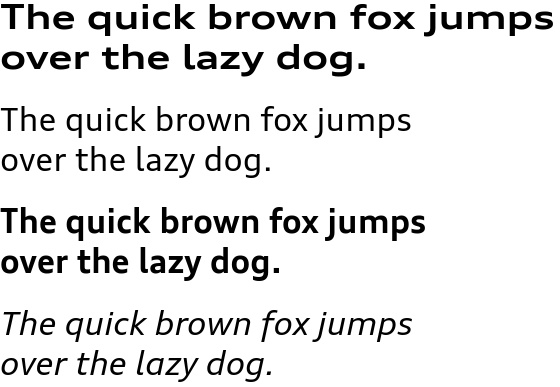
\includegraphics[width=4.5cm,height=3cm]{audi.png}
                \end{center}
                        \caption{Audi Type Variable Typeface}
                \end{subfigure}
	\end{center}
	\end{figure}

	Furthermore, FontAwesome (FontAwesome, 2021) was used in simplifying the user experience by implementing recognizable and relatable symbols in places where text would create too much [bloat] and unnecessary reading. This also aids accessibility and improves navigation. Common uses of these include: identification with location, maps, map features, weather features, personal features, and equipment.\\ 

	Finally; hue, saturation and luminance are all appropriately assigned values to elements of the design to allow optimal readability and minimal strain. When viewing the main portion of the site, the OS map, there isn't much exposed blue light. It is of course, as always, recommended that a user adjusts the gamma output of their display accordingly. Improvement can always be made in areas of accessibility. Some may include JavaScript functionality which allows the user to control the font size, colors, element sizes, etc.; features alike. Given the constraints, brief and target users (myself and a marker), the time-reward trade-off was not valuable.

			\paragraph{Desktop Publishing (DTP)}

	This is an non-required portion of the project and exists to serve a purpose defined long before completion. The promotional piece is out of date however, is still beautiful and is displayed in Figure A5 for your leisure. Note that some additional graphic design features were due to be implemented however, were omitted due to time constraints/relevance. For example, map symbols were all intended to be custom designs however FontAwesome was favoured instead.

			\paragraph{Photo Manipulation}

	The primary use of GIMP in this project was to design an appropriate logo to-be implemented on every page of the site, which relates closely to it's themes. This is seen below in Figure 5.2.

	\begin{figure}[H]
	\begin{center}
		
\includegraphics[width=8cm,height=2cm]{Logo.png}
		\caption{Logo (Made in GIMP)}
	\end{center}
	\end{figure}

\newpage

	The logo considers four relevant layers: text, shape, color, effects. The font (\textit{text}) represents an association with the `outdoor/natural' life theme of the system in it's rustic semi-Sans-Serif nature. \textit{Shape} is used in the 30\textdegree\ slant of the text, representing perceived distortion of space around the user and `natural ([420 B L A Z E $\ast$ I T]) high' experienced while moving at a fast-pace in the field. A red \textit{color} is used in the `burning' word to \textit{harmonize} with the word's semantic definition and \textit{emphasise} the `burning desire' for aspects discussed in the \textit{Introduction} section. A reverse-distress overlay (grunge effect) is used on the `roots' word to \textit{emphasise} the diverse combination of `worn', `distressed', `fatigued', `excited' and `accomplished' emotions experienced by the user in the field. This process is shown below in Figure 5.3.

	\begin{figure}[H]
	\begin{center}
		\begin{subfigure}[t]{6cm}
                \begin{center}
                        
\includegraphics[width=5cm,height=1.25cm]{roots2.png}
                \end{center}
                        \caption{Pre-Grunge}
                \end{subfigure}
                \begin{subfigure}[t]{6cm}
                \begin{center}
                        
\includegraphics[width=5cm,height=1.25cm]{Roots2.png}
                \end{center}
                        \caption{Post-Grunge}
                \end{subfigure}
		\caption{Logo Text Distress Process}
	\end{center}
	\end{figure}

		\subsubsection{Use Cases}

	A use case diagram is irrelevant given the context and structure of the following portions of this report. It's use would be [nugatory] and provide no beneficial context. Hence, referring to all headings under the following \textit{Data Application \& Manipulation} section, the data overview in Figure A4, and functions detailed in Figure A6; use cases involving each unction's relevance to site-present applications can be deduced from this content.

	\subsection{Data Application \& Manipulation}

	All data discussed in Section 4 of this report is included in a basic input-output system [(BIOS, wheyy)] which, through functions and others methods, produces the desired outcomes to satisfy user requirements. A summary of this process can be seen Figure A6. Reference to data can be observed in Figure A4.

		\subsubsection{`Overview'}

	The `Overview' portion of the home page of this site refers to a more basic iteration of the route search and landmass search functions, seen subsequently in the `Conquest Map'. For the sake of continuity, all basic features of these functions' use of data is discussed under this heading; additional data required for the `Conquest Map' version are discussed latterly.

			\paragraph{Score Route}

	This function exists purely to serve the Search Route function and has no purpose as a stand-alone. As it involves quite the lengthy arithmetic process however, it is granted its own sub-sub-sub-section. Although, to my judgement, this metric is fairly mathematically sound although will be constantly developed as I generate more ideas, it is still very subjective and based on my own experiences with and discussions about the Scottish hills and their conditions. Therefore, this `score' is not a definitive metric to describe the condition of a route to the masses. It should be judged and considered on an individual basis.\\

	Scoring a route takes into account [1] four groups of subjective scores based on weights and values of the four route element factors under routes in the JSON file (type, stages, terrain types, terrain difficulties), and [2] a more objective and logical multiplier based on total number of [Munro, `Top, Corbett, `Top] tops covered on-route, the total elevation gained, and the total distance covered. Actual values of the weights were gathered through personal field consideration/conversation and are therefore subject to bias and constant adjustment. The multiplier was developed purely by myself. Parameters follow:

	\begin{enumerate}
	\setlength\itemsep{0cm}
		\item Conversion constants (ft--m, mi--km) -- values
		\item Number of tops -- value
		\item Elevation -- value
		\item Distance -- value
		\item Route type (weight, \{weights, `values'\}, `score') -- matrix
		\item Route stages (weight, \{weights, `values'\}, `score') -- matrix
		\item Terrain types (weight, \{weights, `values'\}, `score') -- matrix
		\item Terrain difficulties (weight, \{weights, `values'\}, `score') -- matrix
	\end{enumerate}

	This site uses the functional imperial system therefore, as this computation calls for the one and only reasonable use of the metric system (mathematical scalability), conversion constants are required for elevation and distance. These are justified to four significant figures. Mathematical notation for each of these processes follow:

\newpage

	\textbf{[1.1] Conversion Constants:}

	$$c_{ft}=0.3048$$
	$$c_{mi}=1.609$$

	Where:\\
	$c_{ft}=$ Conversion constant for imperial feet to metric meters\\
	$c_{mi}=$ Conversion constant for imperial miles to metric kilometers ($\times10^{3}$m)\\

	\textbf{[1.2] Number of Tops:}

	$$N_{\mathrm{Tops}}=\sum^{I}_{i=1}N_{i}+\sum^{J}_{j=1}N_{j}+\sum^{K}_{k=1}N_{k}+\sum^{L}_{l=1}N_{l}$$
	$$\lor\ N_{\mathrm{Tops}}=\vert i\vert + \vert j\vert + \vert k\vert + \vert l\vert$$

	Where:\\
	$N_{\mathrm{Tops}}=$ Total number of tops present on given route\\
	$N_{i,j,k,l}=$ Numerical value representing the position of a string element $i,j,k,l$ in arrays of $i$: route type, $j$: route stages, $k$: terrain types, $l$: terrain difficulties; $i\in\{1,...I\}$, $j\in\{1,...J\}$, $k\in\{1,...K\}$, $l\in\{1,...L\}$\\

	\textbf{[1.3] Elevation:}

	$$\mathrm{Elev}_{m}=c_{ft}\mathrm{Elev}_{ft}$$

	Where:\\
	$\mathrm{Elev}_{m}=$ Total elevation gained on given route, in meters (m)\\
	$\mathrm{Elev}_{ft}=$ Total elevation gained on given route, in feet (ft)\\

	\textbf{[1.4] Distance:}

	$$\mathrm{Dist}_{km}=c_{mi}\mathrm{Dist}_{mi}$$

	Where:\\
	$\mathrm{Dist}_{km}=$ Total distance covered on given route, in kilometers (km)\\
	$\mathrm{Dist}_{mi}=$ Total distance covered on given route, in miles (mi)\\

\newpage

	\textbf{[2.1] Weights:}\\

	For Route Type's, Route Stages', Terrain Types', Terrain Difficulties' Elements\\

	This method defines equally weighted elements by dividing 1 by the number of elements in the arrays. Where $i,j,k,l$ refer to arrays and positions within their respective arrays:

	$$w_{i}=\frac{1}{\sum^{I}_{i=1}N_{i}},\ w_{j}=\frac{1}{\sum^{J}_{j=1}N_{j}},\ w_{k}=\frac{1}{\sum^{K}_{k=1}N_{k}},\ w_{l}=\frac{1}{\sum^{L}_{l=1}N_{l}}$$
	$$\lor\ w_{i}=\frac{1}{\vert i\vert},\ w_{j}=\frac{1}{\vert j\vert},\ w_{k}=\frac{1}{\vert k\vert},\ w_{l}=\frac{1}{\vert l\vert}$$

	$$\therefore w_{i}, w_{j}, w_{k}, w_{l}\ \textrm{always constant and equally weighted}$$

	Where:\\
	$w_{i,j,k,l}=$ Equally weighted value based on number of elements for element $i,j,k,l$ in arrays of $i$: route type, $j$: route stages, $k$: terrain types, $l$: terrain difficulties; $i\in\{1,...I\}$, $j\in\{1,...J\}$, $k\in\{1,...K\}$, $l\in\{1,...L\}$\\
	$N_{i,j,k,l}=$ Numerical value representing the position of a string element $i,j,k,l$ in arrays of $i$: route type, $j$: route stages, $k$: terrain types, $l$: terrain difficulties; $i\in\{1,...I\}$, $j\in\{1,...J\}$, $k\in\{1,...K\}$, $l\in\{1,...L\}$\\

	\textbf{[2.2] Scores:}\\

	For Route Type, Route Stages, Terrain Types, Terrain Difficulties

	$$S_{i}=\sum^{I}_{i=1} w_{i}V_{i},\ S_{j}=\sum^{J}_{j=1} w_{j}V_{j},\ S_{k}=\sum^{K}_{k=1} w_{k}V_{k},\ S_{l}=\sum^{L}_{l=1} w_{l}V_{l},$$

	Where:\\
	$S_{i,j,k,l}=$ Relative score of element $i,j,k,l$ in arrays of $i$: route type, $j$: route stages, $k$: terrain types, $l$: terrain difficulties; $i\in\{1,...I\}$, $j\in\{1,...J\}$, $k\in\{1,...K\}$, $l\in\{1,...L\}$\\
	$V_{i,j,k,l}=$ Subjectively defined value assigned to element $i,j,k,l$ in arrays of $i$: route type, $j$: route stages, $k$: terrain types, $l$: terrain difficulties; $i\in\{1,...I\}$, $j\in\{1,...J\}$, $k\in\{1,...K\}$, $l\in\{1,...L\}$\\

\newpage

	An example for the route type array ($i$) which contains three equally weighted elements follows:

	$$S_{i}=w_{1}V_{1}+w_{2}V_{2}+w_{3}V_{3}$$
	$$S_{i}=\frac{1}{3}\left(\frac{1}{4}\right)+\frac{1}{3}\left(\frac{1}{4}\right)+\frac{1}{3}\left(\frac{1}{2}\right)$$
	$$S_{i}=\frac{1}{3}=0.\textrm{\.{3}}$$
	
	As these values are generated from an array, they involve single-column (no inversion) matrix algebra in the context of JavaScript. An example of the appropriate notation relating to the previous example follows (decimal values favoured in matrices):

	$$S_{i}=\left[0.\textrm{\.{3}}\ 0.\textrm{\.{3}}\ 0.\textrm{\.{3}}\right]\left[0.25\ 0.25\ 0.5\right]$$
	$$S_{i}=0.\textrm{\.{3}}$$

	Again, as this is single-column matrix algebra, standard notation is also viable:

	$$S_{i}=\begin{bmatrix}w_{1}\\w_{2}\\w_{3}\end{bmatrix}\begin{bmatrix}V_{1}\\V_{2}\\V_{3}\end{bmatrix}$$
	$$S_{i}=\begin{bmatrix}0.\textrm{\.{3}}\\0.\textrm{\.{3}}\\0.\textrm{\.{3}}\\\end{bmatrix}\begin{bmatrix}0.25\\0.25\\0.5\end{bmatrix}$$
	$$S_{i}=0.\textrm{\.{3}}$$

	For each of the route element factor arrays, these are then aggregated to give a total value. However, they still do not have any context which is why a multiplier is used.\\

	\textbf{[2.3] Weights:}\\

	For Route Type, Route Stages, Terrain Types, Terrain Difficulties

	$$w_{S_{i}},\ w_{S_{j}},\ w_{S_{k}},\ w_{S_{l}}$$

	Do not confuse these with the equal weightings for each individual element within the arrays, these four weightings exist on a subjective basis to weight the four scores for each array.

	Where:\\
	$w_{S_{i,j,k,l}}=$ Weight values determining the importance of arrays of $i$: route type, $j$: route stages, $k$: terrain types, $l$: terrain difficulties; $i\in\{1,...I\}$, $j\in\{1,...J\}$, $k\in\{1,...K\}$, $l\in\{1,...L\}$\\

	\textbf{[3.1] Complete Multiplier:}

	$$m_{R}=\frac{N_{\mathrm{Tops}}}{\left(\frac{\mathrm{Elev_{m}}}{1000\left(\mathrm{Dist_{km}}\right)}\right)}$$
	$$\textbf{Expanded: }m_{R}=\frac{\sum^{I}_{i=1}N_{i}+\sum^{J}_{j=1}N_{j}+\sum^{K}_{k=1}N_{k}+\sum^{L}_{l=1}N_{l}}{\left(\frac{c_{ft}\mathrm{Elev_{ft}}}{1000\left(c_{mi}\mathrm{Dist_{mi}}\right)}\right)}$$

	Where:\\
	$m_{R}=$ Multiplier for given route $R$\\

	In English, this equation reads: ``number of tops (Munro, Munro Top, Corbett, Corbett Top) achieved on the route per vertical meter gained on the route, per horizontal meter gained on the route''.\\

	\textbf{[3.2] Complete Aggregate Route Score:}

	$$S_{R}=w_{S_{i}}S_{i}+w_{S_{j}}S_{j}+w_{S_{k}}S_{k}+w_{S_{l}}S_{l}$$
	$$\textbf{Expanded (1): }S_{R}=w_{S_{i}}\left(\sum^{I}_{i=1} w_{i}V_{i}\right)+...+w_{S_{l}}\left(\sum^{L}_{l=1} w_{l}V_{l}\right)$$
	$$\textbf{Expanded (2): }S_{R}=w_{S_{i}}\left(\sum^{I}_{i=1} \left(\frac{1}{\sum^{I}_{i=1}N_{i}}\right)V_{i}\right)+...+w_{S_{l}}\left(\sum^{L}_{l=1} \left(\frac{1}{\sum^{L}_{l=1}N_{l}}\right)V_{l}\right)$$

	Where:\\
	$S_{R}=$ Aggregate route score for given route $R$\\

	\textbf{[4] Complete Adjusted Route Score:}

	$$S_{R(A)}=m_{R}\left(w_{S_{i}}S_{i}+w_{S_{j}}S_{j}+w_{S_{k}}S_{k}+w_{S_{l}}S_{l}\right)$$

	$$\textbf{Expanded (1):}$$
	$$S_{R(A)}=\left(\frac{N_{\mathrm{Tops}}}{\left(\frac{\mathrm{Elev_{m}}}{1000\left(\mathrm{Dist_{km}}\right)}\right)}\right)\left(w_{S_{i}}\left(\sum^{I}_{i=1} w_{i}V_{i}\right)+...+w_{S_{l}}\left(\sum^{L}_{l=1} w_{l}V_{l}\right)\right)$$
	$$\textbf{Expanded (2):}$$
	$$S_{R(A)}=\left(\frac{\sum^{I}_{i=1}N_{i}+\sum^{J}_{j=1}N_{j}+\sum^{K}_{k=1}N_{k}+\sum^{L}_{l=1}N_{l}}{\left(\frac{c_{ft}\mathrm{Elev_{ft}}}{1000\left(c_{mi}\mathrm{Dist_{mi}}\right)}\right)}\right)$$
	$$\bullet\left(w_{S_{i}}\left(\sum^{I}_{i=1} \left(\frac{1}{\sum^{I}_{i=1}N_{i}}\right)V_{i}\right)+...+w_{S_{l}}\left(\sum^{L}_{l=1} \left(\frac{1}{\sum^{L}_{l=1}N_{l}}\right)V_{l}\right)\right)$$

	Where:\\
	$S_{R(A)}=$ Adjusted route score for given route $R$\\

	In English, this equation reads: ``number of tops (Munro, Munro Top, Corbett, Corbett Top) achieved on the route per vertical meter gained on the route, per horizontal meter gained on the route; scaled by the route type, route stages, terrain types, and terrain difficulty elements found on-route''.\\

	Given the time constraint of the project, some restrictions have been applied and notes made, as follows:

	\begin{itemize}
	\setlength\itemsep{0cm}
		\item Writing the score route function would be too-lengthy-a-process if calculating the score of each of the four route elements based on the individual values of the 5, 4, 11 and 20 sub-elements respectively using the factorial method, so the latter 3 are calculated simply by volume/variety. This does not accurately reflect the difficulty of terrain for example as a route with grass and concrete will be considered more difficult than a route with grade 3 slab, simply because it has one more element. In this context it doesn't matter too much as the math has been demonstrated successfully however.
		\item If using the exhaustive method, volume is accounted for by the inclusion and exclusion of values which, if all-inclusive, should add up to N sub-elements in that group. But this is rare.
		\item All four of the route elements do not include consistent examinations of their sub-elements (value ($V_{i,j,k,l}$)) when scoring a route. That is, for example using the route type array, sub-element $i=1$ and $i=5$ may not be examined together if they do not appear as a combination in the JSON file and therefore don't critically need to be examined. Equally, in the route stage array, perhaps sub-element $j=3$ isn't examined soley because it doesn't appear on its own in the JSON file. In a perfect world, every combination and isolation would be examined however, with the time allocated here, it is not worth the effort.
	\end{itemize}

			\paragraph{Describe Route Score}

	This is a small function which is used simply to evaluate the meaning of the given route score and translate it into more appropriate and understandable human terms. It's based on multiple increments from 0--100+, including: 0-33.\.{3}: ``Playground (Amateur)''; 34--66.\.{6}: ``Normie (Easy)''; 67--100: ``Trad (Moderate)''; 100+: ``GigaChad (Challenging)''. It gives the user a slightly better indication of their what the route requires from their ability.

			\paragraph{Search Route}

	This function searches JSON [1] (Figure A4) for data under a \texttt{landmass} $\rightarrow$ \texttt{route} for a match with input from a two-tier HTML \texttt{select} process. The first \texttt{select} allows the user to choose their desired landmass from their names matching those in the JSON file. Once an \texttt{option} has been selected, a relevant element is generated which displays the second \texttt{select} process that allows users to view and select from routes, matching those with names in the JSON file, on their selected landmass. This process could of course be executed using a manual text \texttt{input} process however, this relies on the user having pre-existing knowledge of landmasses and their routes and takes away from the comprehensiveness and inclusiveness of allowing them to view all possibilities. Essentially, this function outputs a body of text which fetches and displays the different attributes of routes in a human-readable context, including a mathematically computed unique and elegant `route score' and the option to download the route's GPX file. This is the fasted method I have witnessed from landing on a site to being able to access a route, download it and use it.

			\paragraph{Search Landmass}

	This function searches JSON [1] (Figure A4) for data under a \texttt{landmass} $\rightarrow$ \texttt{munro}, \texttt{munrotop}, \texttt{corbetttop} or \texttt{corbett} for a match with input from an HTML text \texttt{input} process. This input allows users to choose their desired hill which appears on a landmass; landmasses are looped until a Munro, Munro Top, Corbett or Corbett Top name appearing under a landmass is matched with the user's input. Note two things: search criteria does not have to be character-matching, case-matching or syntactically correct as there is JavaScript protocol in place to ensure more `loose' data matching; and [2] if there are multiple matches under a user input, results are prioritized firstly by landmass appearance in the JSON file (as landmasses are ordered south-to-north and the majority of users will live south of the highlands, this will produce a more logical results), and secondly by hierarchy of peak (Munro, `Top, Corbett, `Top) according to their ordering in the file (which is also logical as users most often are searching for Munros). This function outputs a body of text which fetches and displays attributes of hills and the landmasses on which they appear, in a human-readable context. Also included is an image of the hill.

		\subsubsection{`Conditioning'}

	The `Conditioning' portion of the home page of this site presents the user with the ability to [1] view `Ability' attribute, and [2] view `Equipment' attributes. This, like the `Overview' section is a simplified and more informative version of what the user will see and use ability and equipment data for in the `Conquest Map'.

			\paragraph{Search `Ability' \& `Equipment'}

	Users are presented with two initial separate HTML \texttt{select} protocol on a two-tier basis (four total \texttt{select} protocol) for each of the `Ability' and `Equipment' sections. The first allows them to choose an \texttt{option} based on which set of ability/equipment factors they wish to inspect, such as hill and route elements, summit features, route types and stages, terrain types and difficulties, etc.; and packs, technical equipment, footwear and clothing, etc. This generates the second \texttt{select} protocol which displays the individual factors under each heading. When the user selects a factor, the element is matched by a loop through the relevant JSON file for the seven ability headings or four equipment headings and a body of text is then generated summarizing the attributes. This includes all of the basics such as brief descriptions and images, etc. This feature is informative and serves no dynamic function until `Conquest Map'.
	
		\subsubsection{`Weather'}

	Fetching and putting weather data to use only requires two parameters: latitude and longitude (\texttt{lat}, \texttt{lon}). This leaves huge opportunity to relate these parameters to many different variables and therefore, many different human-interpreted scenarios. Accepted in the weather system are four different methods of acquiring input of latitude and longitude values. The first is two \texttt{select} options which list Munros, Corbetts and regions and loop the relevant JSON file for a match then relay their \texttt{lat} and \texttt{lon} attributes to input. The second is a search feature much like that seen in the `Overview' section where the user can search loosely for the names of Munros and Corbetts and have their attributes captured from the JSON file. Thirdly, the user can use a Geolocation function to fetch their current coordinates and have them entered directly into the script. Finally, there is the option to manually input latitude and longitude directly into the \texttt{input} boxes. This is possible as the script takes its \texttt{lat} and \texttt{lon} inputs directly from the values of these input boxes which are displayed on the UI.\\

	As seen in Figure A4, most data which is fetched using the OpenWeather API is displayed directly on the UI witch some form of string, symbol and CSS design aspects to contextualize them. However, there are some components such as [1] the day and time (daily and hourly), [2] sunrise time, [3] sunset time, [4] precipitation (daily and hourly) and [5] visibility which require some basic arithmetic and JavaScript conversions to be presentable. This extends no further than one line of code however. Further, there are several components which do not exist as part of the OpenWeather API and require more complex computations based on aspects of the API. These include [1] inspecting the complete range weather icon provided by OpenWeather and reassigning icon values to custom ones (daily and hourly); [2] assigning string descriptions of wind direction\footnote{The direction \textit{from} which the wind is travelling (originates)} at different angular intervals of wind direction provided by OpenWeather (daily and hourly)\footnote{Note there were no precise-enough sources supplying these intervals so much effort with a calculator was devoted}; and [3] assigning an arrow symbol and computing a CSS angular rotation value relative to the wind direction (daily and hourly). This symbol is provided by the Version 5 FontAwesome Free Library (FontAwesome, 2021). Demonstrations of how these are implemented are highlighted in Table 5.2 below. The four basic computations can be seen in Figure A4. These computations also include various alike calculations relevant to CSS, for example, to color the background of the temperature section at different increments and change the font color accordingly, etc.

\newpage

	\begin{center}
		\scriptsize
	\begin{longtable}{p{12cm}}
		\hline
		\multicolumn{1}{c}{\textsc{Weather Icons}}\\
		\hline
		\begin{lstlisting}
let wicon = "";
for (var i in day.weather) {
	if (day.weather[i].icon === "01d") {
		wicon = "<i class='fas fa-sun'></i>";
	} else if (day.weather[i].icon === "01n") {
		wicon = "<i class='fas fa-moon'></i>";
	...
	} else if (day.weather[i].icon === "50d") {
		wicon = "<i class='fas fa-smog'></i>";
	} else if (day.weather[i].icon === "50n") {
		wicon = "<i class='fas fa-smog'></i>";
	}
}
		\end{lstlisting}\\
		\hline
		\multicolumn{1}{c}{\textsc{Wind Direction Description}}\\
		\hline
		\begin{lstlisting}
let day_wind_dir = "";
if ((day.wind_deg) >= 348.76) {
	day_wind_dir = "N";
} else if ((day.wind_deg) >= 0 && (day.wind_deg) <= 11.25) {
	day_wind_dir = "N";
} else if ((day.wind_deg) >= 11.26 && (day.wind_deg) <= 33.75) {
	day_wind_dir = "N/NE";
} else if ((day.wind_deg) >= 33.76 && (day.wind_deg) <= 56.25) {
	day_wind_dir = "NE";
...
} else if ((day.wind_deg) >= 303.76 && (day.wind_deg) <= 326.25) {
	day_wind_dir = "NW";
} else if ((day.wind_deg) >= 326.26 && (day.wind_deg) <= 348.75) {
	day_wind_dir = "N/NW";
}
		\end{lstlisting}\\
		\hline
		\multicolumn{1}{c}{\textsc{Wind Direction Symbol}}\\
		\hline
		$$\angle=(-45)+180+W$$\\
		Where:\\
		$\angle=$ Angle Assigned to CSS Rotate of Object (\textdegree) (no variable name as used directly in-line)\\
		$W=$ Wind Direction (\textdegree) $=$ \texttt{hour.wind\_deg} (as named in the OpenWeather API)\\
		`$-45$' accounts for the 45\textdegree\ visual offset as standard design in the symbol (return to 0\textdegree)\\
		`$+180$' accounts for the `direction from which the wind is travelling' and rotates the symbol by 180\textdegree\ to point the nose of the arrow in the opposite direction which symbolizes the `direction in which the wind is travelling'\\
		\hline
		Note that these examples are extracted from `daily' weather forecasting. Near-identical code is replicated for the `hourly' equivalent.\\
		\hline
		\caption{Weather System Computations}
	\end{longtable}
	\end{center}

		\subsubsection{`Conquest' Map}

	The `Conquest Map' is the heart of this system. It uses the Ordnance Survey Leisure Map API (OS API) (Ordnance Survey, 2022) to display a base map, along with other JavaScript features such as use of the Leaflet (Leaflet, 2022) library and others noted in the \textit{System Construction} section, upon which many previously discussed, and further layers of, data is processed and displayed using various methods and forms of media.

			\paragraph{Change Map Layer}

	A basic three-option \texttt{radio} input feature is available to the user as soon as they enter the page, giving them the option to fetch three different sets of base map layer data from the OS API: `Leisure', `Road', `Outdoor'. These are the three most relevant topographical maps to the data displayed.

			\paragraph{Show Current Location \& Find Nearest}

	An array of two \texttt{button}s are presented which call functions that display the current location of the user's device and find the nearest hill to the user, respectively. The first of these uses the Geolocation API to fetch the \texttt{lat} and \texttt{lon} attributes and inputs then into a function which outputs the user's location by [1] centering the map crosshair to the coordinates, [2] creating and displaying a marker upon this location, and [3] calculating and presenting an accuracy/tolerance radius around this. Finding the nearest hill involves a similar process in that it fetches the user's coordinates using Geolocation and inputs them into a function which takes into account the coordinates of all routes in the relevant JSON file (Figure A4) and calculates their distance form the current coordinates. It then displays a hill as standard; it's markers, and pop-ups etc., are discussed under section 5.3.4.8

			\paragraph{Show \& Hide Features}

	An array of four \texttt{button}s are presented which call functions that display markers for all Munros, Munro Tops, Corbetts, Corbett Tops, and hide all markers, respectively. These functions operate in a near-identical manner, in which they loop the relevant JSON file to fetch the \texttt{lat} and \texttt{lon} values of all the iterations of either \texttt{munro}, \texttt{munrotop}, \texttt{corbett}, or \texttt{corbetttop}. The output is the creation and display of a Leaflet marker for every hill relative to the button selected, with a bound Leaflet pop-up which accepts inputs such as the name and different statistics and images of the hill from the JSON file, and is displayed upon click [of the marker]. The `hide' function simply loops through the array used to store the markers upon creation and removes their relative layer from the map.

			\paragraph{Filter Routes By `Ability' \& `Equipment'}

	See section 5.3.2.1 for the breakdown of these components. After the user makes their relevant selections from the relevant HTML \texttt{select} protocol, instead of having all of the attributes of the associated matched items in the JSON file simply printed in a body of text, the selections are added to a pool. The values of this this pool (which are elements of ability and equipment) are then matched with routes under the landmasses of the appropriate JSON file. Once the user submits their request, all routes which either \textbf{do} or \textbf{do not} contain these attributes, based on the user preference through a \texttt{radio} input feature, are located in the appropriate JSON file. It then displays all of these routes as standard; route markers, lines, hill markers and pop-ups etc., are discussed under sections 5.3.4.7 and 5.3.4.8. Unlike when seeking an individual route, the map crosshair is not centered to any particular route as there may be more than one.

			\paragraph{Score Route}

	See section 5.3.1.1 for the breakdown of this component. No attributes differ.

			\paragraph{Describe Route Score}

	See section 5.3.1.2 for the breakdown of this component. No attributes differ.

			\paragraph{Search Route}

	See section 5.3.1.3 for the breakdown of this component. There are additional features implemented in this function, in the relevance of the `Conquest Map'. The user is presented now with four options instead of just the original `summary' option under `Overview'. They are: [1] present a summary of the route as detailed in section 5.3.1.3, [2] print the route, [3] hide all routes, and [4] begin a `\href{https://www.youtube.com/watch?v=IvaldKgWGHo}{Galactic Conquest}'.\\

	The print route function essentially uses the same data from the JSON file as the summary function however, it uses the GPX suffix attribute of the selected route to match with an appropriate prefix. The file matching this path is then fetched and loaded by the function using the GPX to GeoJSON method, as this is a more appropriate use in JavaScript. This GPX data is then printed on the map. Secondly, the function calls another function discussed earlier which prints a route (Leaflet) marker. This marker contains a bound Leaflet pop-up which, upon click, displays variations of data displayed in the original route search output. Finally, the function also makes calls to other functions to which attributes names of hills appearing on the route are relayed and appropriate Leaflet markers are displayed. These functions behave similarly to those discussed in section 5.3.4.2, except this time they do not print all of the Munro, `Top, Corbett and `Top markers, they just print the relevant ones.\\

	The hide all routes function acts much like the hide the function used to hide all hill markers. It simply loops through the array used to store the routes upon creation and removes their relative layer from the map. This includes all of the route markers, lines and hill markers. The fourth and final option, `Galactic Conquest' is a meme which simply loops through the entire JSON file, collects every GPX attribute suffix, matches with the appropriate prefix, and prints them on the map with the appropriate route markers, lines and hill markers.

			\paragraph{Search Landmass}	

	See section 5.3.1.4 for the breakdown of this component. There are additional features implemented in this function, in the relevance of the `Conquest Map'. As well as printing the body of text with the summary of all the attributes like before, this function also uses the \texttt{lat} and \texttt{lon} attributes of the hill firstly to input into another function which calculates the hill's distance from the user's current location and display this as part of the body-text output; and secondly, to center the map crosshair to the hill's location; and, calls a function which creates a single hill marker for the appropriate hill. This marker follows the same structure as those detailed in sections 5.3.4.4 and 5.3.4.7, except this time it prints only the single relevant Munro, `Top, Corbett or `Top.

\newpage

\section{System Construction}\label{ch6}

	The goal in selecting methods through which to construct this system is aligned with [1] ensuring that all functional and non-functional requirements detailed in the \textit{System Requirements} section, determined by and for potential clients, are satisfied; and [2] all components of used to build the system work harmoniously to deliver the most efficient delivery, to the developer's (my) best knowledge and ability.

	\subsection{Requirements Satisfaction}

	Referring to sub-sub-sections 3.3.1 and 3.3.2 under the \textit{System Requirements} section, and user stories seen in Figure A3; and applying their relevance to data and functions detailed in Figures A4 and A6, respectively; requirements are satisfied as follow in Table 6.3.

	\begin{center}
		\scriptsize
	\begin{longtable}{ccp{5.5cm}p{5.5cm}}
		Req. \# & Status & Satisfaction(s) & Extension(s)\\
		\hline
		\multicolumn{4}{c}{\textsc{Functional}}\\
		\hline
		1$^M$ & Y & Weather app$^{W,G}$, \texttt{getLatLon()}$^G$, \texttt{findLocation()}$^G$, \texttt{showLocation()}: use current location in weather app, find latitude and longitude of user's device, find current coordinates for map, print current coordinates as a marker on map & \texttt{showNearest()}, \texttt{getDistanceCurr()}: find nearest hill to current coordinates, find distance form current coordinates marker to variable marker\\
		2$^M$ & Y & \texttt{searchRoute()}: search for and display defined route data from the JSON file & \texttt{scoreRoute()}, \texttt{describeRoute()}, \texttt{searchLocation()}: compute a relative route score based on a mathematical algorithm, describe the route score based on the algorithmic results, search individual locations from the JSON file which appear isolated and as members of routes\\
		3$^M$ & Y & \texttt{searchAbility()}: search for and display defined ability data from the JSON file & \texttt{refineRouteAbility()}: refine routes by declaring ability-based inputs\\
		4$^M$ & Y & \texttt{searchEquipment()}: search for and display defined equipment data from the JSON file & \texttt{refineRouteEquipment()}: refine routes by declaring equipment-based inputs\\
		5$^M$ & Y & Weather app$^{W,G}$: display `tiles' of daily and hourly weather data with current location as a location option & \texttt{selectMunroOpt()}, \texttt{inpMunroOpt()}, \texttt{selectCorbettOpt()}, \texttt{inpCorbettOpt()}, \texttt{selectCounty()}: select Munro to fetch and pass coordinates, input Munro to fetch and pass coordinates, select Corbett to fetch and pass coordinates, input Corbett to fetch and pass coordinates, select county to fetch and pass coordinates (... from JSON file ... to weather app)\\
		6$^M$ & Y & `Conquest Map'$^O$, \texttt{findLocation()}$^G$, \texttt{showLocation()}, \texttt{createHillMarker()}, \texttt{createRouteMarker()}, \texttt{hideMarkers()}, \texttt{getLatLon()}$^G$, \texttt{getDistanceCurr()}, \texttt{getDistance()}, \texttt{searchRoute()}, \texttt{showRoute()}, \texttt{hideRoutes()}: find current coordinates for map, print current coordinates as a marker on map, print hill coordinates on map, hide hill markers, find latitude and longitude of user's device, find distance form current coordinates marker to variable marker, find distance from variable marker to variable marker, search for and display defined route data from the JSON file, display GPX data of route with other components, hide route GPX data and components & \texttt{showNearest()}, show pan coordinates, \texttt{showMunros()}, \texttt{showMunroTops()}, \texttt{showCorbetts()}, \texttt{showCorbettTops}, , \texttt{showMunro()}, \texttt{showMunroTop()}, \texttt{showCorbett()}, \texttt{showCorbettTop()}, \texttt{searchAbility()}, \texttt{searchEquipment()}, \texttt{refineRouteAbility()}, \texttt{refineRouteEquipment()}, \texttt{scoreRoute()}, \texttt{describeScore()}, \texttt{searchLocation()}, \texttt{galacticConquest()}: find nearest hill to current coordinates, print all Munro coordinates on map, print all Munro Top coordinates on map, print all Corbett coordinates on map, print all Corbett Top coordinates on map, print defined Munro coordinates on map, print defined Munro Top coordinates on map, print defined Corbett coordinates on map, print defined Corbett Top coordinates on map, search for and display defined ability data from the JSON file, search for and display defined equipment data from the JSON file, refine routes by declaring ability-based inputs, refine routes by declaring equipment-based inputs, compute a relative route score based on a mathematical algorithm, describe the route score based on the algorithmic results, search individual locations from the JSON file which appear isolated and as members of routes, display GPX data of all routes with other components\\
		1$^S$ & Y & \texttt{switchLayer()$^O$}: change OS map base layer choosing from `OS Leisure', `OS Road' and `OS Outdoor' & N/A\\
		2$^S$ & Y & Center crosshair: display icon panning with the center of the map upon \texttt{move} & Pan coordinates: display panning latitude and longitude upon event \texttt{move}\\
		1$^C$ & N & N/A: No database back-end & N/A\\
		2$^C$ & N & N/A: No existing user data as no database back-end & N/A\\
		3$^C$ & N & N/A: No existing user data as no database back-end & N/A\\
		4$^C$ & N & N/A: No existing user data as no database back-end & N/A\\
		1$^W$ & N & N/A: `Wont Have' requirement & N/A\\
		\hline
		\multicolumn{4}{c}{\textsc{Non-Functional}}\\
		\hline
		1 & Y/P & Written using HTML5, CSS and JavaScript which are supported by all modern browsers. Therefore, all basic necessary content loads for the majority of users & Includes some external scripts references to libraries such as Leaflet, and FontAwesome. Leaflet rarely causes trouble however, some browsers do not support variations and iterations of FontAwesome symbols and generations\\
		2 & Y & CSS included to ensure all elements which can be seen on the desktop site are visible clearly when scaled to mobile & Some elements are re-styled to add more `mobile friendly' and relevant interactivity\\
		3 & Y & The `Overview', `Conditioning', `Weather' and `Conquest Map' all include elements such as search functions, `keys' and `suggested readings' which are purely informative in aiding knowledge and understanding of other functions of the site & N/A\\
		4 & Y & As discussed, appropriate CSS is applied to make the site relevant to the theme and widely accessible & As discussed, graphic design, photo manipulation and non-essential CSS elements are included to further enhance the experience and enjoyment on the site\\
		5 & Y & As discussed above, CSS standard adhere to required accessibility standards & N/A\\
		\hline
		\multicolumn{4}{p{12cm}}{Y: Yes, Satisfied; N: No, Not Satisfied; P: Partially Satisfied\newline <...>, <...>: ``...'', ``...'' under \textit{Satisfaction(s)} and \textit{Extension(s)} are syntactically respective\newline $^G$: Geolocation API; $^O$: OS API; $^W$: OpenWeather API (Prioritized script by relevance)}\\
		\hline
		\caption{Requirements Satisfaction}
	\end{longtable}
	\end{center}

\newpage

	\subsection{Development \& Languages}

	Table 6.4 below details all of the languages, packages, libraries, APIs and development environments used throughout this development process; chosen by the developer (myself) to make the process as efficient and relevant to existing knowledge as possible. As a note, many would recommend the use of React.js JavaScript library in this development process due to its wide scope of JavaScript and JSON capabilities relevant to this site however, the goal was to stay minimal and efficient.

	\begin{table}[h]
		\scriptsize
		\renewcommand{\arraystretch}{1.25}
	\begin{center}
	\begin{tabular}{l|p{1.75cm}p{2.25cm}p{2cm}p{3.5cm}}
		\textsc{Application} & \textsc{Languages} & \textsc{APIs} & \textsc{Lib./Scripts} & \textsc{Environment}\\
		\hline
		\hline
		UI Functionality & HTML\newline JavaScript & Geolocation\newline Open Weather\newline Ordnance Survey & Leaflet\newline Mapbox\newline Chart.js$^1$ & Command Line\newline \rotatebox[origin=c]{180}{$\Lsh$} Vim\newline \rotatebox[origin=c]{180}{$\Lsh$} \texttt{.html}, \texttt{.js}\\
		\hline
		UI Style/Design & CSS & N/A & FontAwesome & Command Line\newline \rotatebox[origin=c]{180}{$\Lsh$} Vim\newline \rotatebox[origin=c]{180}{$\Lsh$} \texttt{.css}\\
		\hline
		Supporting Data & JSON & N/A & N/A & Command Line\newline \rotatebox[origin=c]{180}{$\Lsh$} Vim\newline \rotatebox[origin=c]{180}{$\Lsh$} \texttt{.json}\\
		\hline
		Graphic Design & N/A & N/A & N/A & Windows 7 Program\newline \rotatebox[origin=c]{180}{$\Lsh$} Serif Page Plus X9\newline \rotatebox[origin=c]{180}{$\Lsh$} \texttt{.pdf}, \texttt{.jpg}\\
		\hline
		Photo Manipulation & N/A & N/A & N/A & Linux Program\newline \rotatebox[origin=c]{180}{$\Lsh$} GIMP\newline \rotatebox[origin=c]{180}{$\Lsh$} \texttt{.png}, \texttt{.jpg}\\
		\hline
		Transcription & N/A & N/A & N/A & Command Line\newline \rotatebox[origin=c]{180}{$\Lsh$} Vim\newline \rotatebox[origin=c]{180}{$\Lsh$} \texttt{.tex}\newline \rotatebox[origin=c]{180}{$\Lsh$} (PDF){\LaTeX}/(\textsc{Xe}){\LaTeX}\newline \rotatebox[origin=c]{180}{$\Lsh$} \texttt{.pdf}\\
		\hline
		Document Distribution & N/A & N/A & N/A & Command Line\newline \rotatebox[origin=c]{180}{$\Lsh$} neoMutt\\
		\hline
		Version Control & CLI Shell & N/A & N/A & Command Line\newline \rotatebox[origin=c]{180}{$\Lsh$} GitHub CLI\\
		\hline
		\hline
		\multicolumn{5}{l}{$^1$: Not used, discussed latterly}\\
		\hline
	\end{tabular}
		\caption{Development Components}
	\end{center}
	\end{table}

\newpage

		\subsubsection{System Directory Tree}

	The following directory tree in Figure 6.4 maps the comprehensive structure of this system. Lower-tier files under `Audi' font, `aonach\_eagach' GPX, `udlaidh\_bhreac-liath' GPX and Leaflet images are omitted. However, directories are exhausted although they do include floating values denoted by ellipses (...) from $1$ to $N$ in their respective list. It of course does not include documentation such as this report.
	
	\begin{figure}[H]
	%\renewcommand*\DTstyle{}
	\DTsetlength{0.5em}{2em}{0.2em}{0.5pt}{1.5pt}
	\dirtree{%
		.1 ./.
			.2 burning.css.
			.2 Conquest.html.
			.2 Fonts.
				.3 Audi.
				.3 NFS.ttf.
			.2 GPX.
				.3 aonach\_eagach.
				.3 ....
				.3 udlaidh\_bhreac-liath.
			.2 index.html.
			.2 JSON.
				.3 abilityEquipment.json.
				.3 Hills.json.
				.3 schema.json.
			.2 Leaflet.
				.3 images.
				.3 ....
				.3 leaflet.js.map.
			.2 Photos.
				.3 Conditioning.
				.3 ....
				.3 Weather.
			.2 Scripts.
				.3 abilitiesEquipment.js.
				.3 ....
				.3 Weather.js.
	}
	\caption{System Directory Tree}
	\end{figure}

		\subsubsection{Development Environment}

	Throughout this development process, there appears no use of any proprietary software as it remains an unreliable, unnecessary, expensive and bloated method of completing tasks. Especially those which may be executed using, for example, one command in the command line or in Vim; or, a set of processes which may be executed more efficiently using, for example, a widely applicable Vim command. Using [free and open source software] such as the operating system ([Artix Linux]), environment (command line / Vim), APIs and libraries significantly increases freedom and extensibility of the project. Hence, the use of dwm's window tiling manager to allow efficient, continuous and conjunctive writing of HTML, CSS, JavaScript and {\TeX}\ documents alongside browser testing (Brave Browser). Any supporting non-essential documentation such as notes are written in plain text (\texttt{.txt}) files using Vim and comma-separated (\texttt{.csv}) files using SC-IM. [All. Plain. Text.]

		\subsubsection{User Interface}

	HTML (HTML5) is used to create the base functionality of this system as it supports all necessary APIs and external scripts. HTML also allows integration of appropriate external stylesheets such as those used to support access to FontAwesome. A minor non-noted script is used to allow the use of {\TeX}\ syntax when writing supporting content such as formul\ae. Furthermore, the benefits of using CSS (CSS3) include: design, scalability and accessibility factors and have been previously discussed. A CSS-less site may be more functional and relatable however, good CSS takes a system from a plain website to a relevant web application. Furthermore, JavaScript ties-in the interactivity and manipulation of the APIs. A combination of external and local scripts are used to [1] make the APIs functional, and [2] make them relevant, respectively. Additionally, there are smaller JavaScript elements throughout the system which do not relate to pure functionality and serve purposes such as the manipulation of CSS and styling elements, etc. Serif Page Plus X9 and GIMP are used in Windows 7 and Artix Linux respectively for graphic design and photo manipulation purposes as previously discussed.

		\subsubsection{Supporting Data}

	JavaScript Object Notation (JSON) files are included to store relevant data as previously discussed, and detailed in Figure A4. They interact with elements of JavaScript scripts to allow access to, fetching of, and use of relevant data for computations and output on the site. If the site were to be expanded in the future to contain user data and a log-in system for example, supporting data would extend to a collection of CSV (\texttt{.csv}) files, and various PHP (\texttt{.php}) and SQL (\texttt{.sql}) protocol. These would be used to write, store, organize/manage and access (read) larger-scale data and requests.

	\subsection{Application Programming Interfaces \& Libraries}

	Application Programming Interfaces (APIs) and JavaScript libraries are included in the development process of this system in order to use and build upon unique layers of existing web material and interface with them using various, in some cases, [free and open-source] JavaScript libraries. Libraries of course being additional pre-defined functions and methods etc., which can be used with the addition of various scripts and stylesheets in order to enable and initialize use of APIs.

		\subsubsection{Geolocation}

	The Geolocation API (Geolocation, 2022) is used to access the current latitude and longitude of the user's device. This has many applications, as detailed in Table 6.3 and Figure A6, such as displaying the user's current coordinates as a string, calculating distances, fetching weather data for the user's current location, displaying the user's current coordinates on a map, etc.

		\subsubsection{Open Weather}

	The OpenWeather API (OpenWeather, 2022) is used to provide access to a comprehensive collection of weather statistics in a JSON format. It includes minutely, hourly and daily data; of which, hourly and daily are used in querying and presentation in the `Weather' section (weather app).

		\subsubsection{Ordnance Survey (OS)}

		The Ordnance Survey (Ordnance Survey, 2022) API is a topographical map API, used in conjunction with Leaflet (section 6.3.4), to display and produce base map layers in a website. Used in this context are \textit{Leisure} maps: OS Road (1 : 250 000), OS Landranger (1 : 50 000) and OS Explorer (1 : 25 000); \textit{Road} maps 1 : 50 000 and 1 : 25 000; and \textit{Outdoor} maps 1 : 50 000 and 1 : 25 000. Note that this API did require some adjustment upon initiation. As this system is primarily based on the Leisure map, it uses the EPSG:27700 coordinate system. Therefore, the origin point of the map layer required manual calibration in order to function with the iconic 1984 EPSG:4326 system; to which all associated GPX, GeoJSON and JSON relate.
		
		\subsubsection{Leaflet}

		Leaflet (Leaflet, 2022) is a JavaScript library used to produce and manipulate map layers from a map API. It's used in this context for the majority of the functionality under the `Conquest Map', as discussed in various sections and appendices throughout this report.

		\subsubsection{Mapbox GL-JS}

		A Mapbox GL-JS (Mapbox, 2022) script was used in this site for the conversion of GPX files to GeoJSON when being read in JavaScript scripts. This is an essential component at the stage where route GPX files are read and thus [1] printed as a Leaflet line on the map, and [2] used to determine the start coordinates of a route in order to produce a Leaflet marker for that location.

		\subsubsection{Chart.js}
	
		Chart.js (Chart.js, 2022) is a JavaScript library for graphing statistics. It was originally intended for use in the `Ranger' section of the site, which would have acted as another page equivalent to the `Conquest Map' based on user-input-based data analysis. Some of it's features would also be available to view and used to manipulate route searching in `Conquest Map', much like `Ability' and `Equipment'.\\

		The separate graphing page, or `calculator', would have included features based on elevation profile, speed input, power input, heart rate input, etc., which could be analysed through the graphing and charting of protocol such as the following:

		\begin{itemize}
		\setlength\itemsep{0cm}
			\item Select: constant speed (max); Output: required time and power
			\item Select: constant speed (average); Output: required time and power
			\item Select: constant power Output; Output: required speed and time
			\item Input: target speed; Output: Required time and power
			\item Input: target power output; Output: required time and power
			\item Input: target energy output; Output: required time and power
		\end{itemize}

		As previously noted, this portion was omitted due to time constraints and lack of relevance to the brief. Although it could make a future appearance beyond the constraints of this project.

\newpage

	\subsection{Project Management}

	The primary goal in constructing this site remains to be the delivery of a functional web application, relative to the brief and requirements, by the project deadline in August. To ensure that the appropriate time and resources are allocated to each segment of the system's construction, continuous planning and documentation was applied. Not extensively or in any professional manner however, as this is still a [solo project]. This process does ensure a clear understanding of resource/environment management, system layers, and the scale and scope of elements.

		\subsubsection{Life-Cycle}

	No formal framework is used in this scenario. However, the project is divided into intuitive sections which segment: project planning; gathering of supporting data; user interface functionality and data use; and, continuous testing and documentation. With reference to the testing stages, each element developed is tested as soon as is necessary by the developer (myself), to instantly correct minor issues. In the latter stages, the system is tested as-a-whole by myself and externals, and analysed in more depth. This style of testing does indeed have some relevance to the `sprint' concept of `Agile' in that project stages are assigned periods which involve continuous reference to the user-centered approach of requirements and testing. Each stage of this also considers the discussed MoSCoW hierarchy.\\

	Throughout this project I adhere to a very minimal and efficient schedule kept using my [Calcurse] calendar client. An overview of this schedule can be seen in the below GANTT Chart, in Table 6.5. It illustrates all of the major project aspects listed above. Note that a chart such as this is always subject to amendment. This illustrative method is useful for both milestones and available tolerances. The chart runs from the dedicated project timespan: the first full week in May (w/c 2$^\textrm{nd}$) until the final full week in July (w/e 31$^\textrm{st}$) (13 weeks). Secondly, I maintain a plain text notes file which allows me to clearly list `to-do' items, issues, constraints, test results, and things alike; for review, amendment and write-up at a later date.

	\vspace{\fill}

	\begin{center}
		\textsc{Turn \& Rotate Page}
	\end{center}

\begin{landscape}

        \begin{table}[h]
                \tiny
                \renewcommand{\arraystretch}{1.25}
        \begin{center}
        \begin{tabular}{rll|cccccccccccccc}
                \textsc{\#} & \textsc{Task} & \textsc{Tools} & \textsc{W1} & \textsc{W2} & \textsc{W3} & \textsc{W4} & \textsc{W5} & \textsc{W6} & \textsc{W7} & \textsc{W8} & \textsc{W9} & \textsc{W10} & \textsc{W11} & \textsc{W12} & \textsc{W13}\\
                \hline
                \textbf{1} & \textbf{Project Planning} &\\
		1.1 & Requirements Gathering & [Big-Brain] & \cellcolor{gray}\\
		1.2 & Requirements Implementation Planning & [Big-Brain] & \cellcolor{gray}\\
		1.3 & Continuous Documentation & [Big-Brain], Calcurse, Text Files & \cellcolor{gray} & \cellcolor{gray} & \cellcolor{gray} & \cellcolor{gray} & \cellcolor{gray} & \cellcolor{gray} & \cellcolor{gray} & \cellcolor{gray} & \cellcolor{gray}\\
		1.4 & Requirements Review & [Big-Brain] & & \cellcolor{gray}\\
                \hline
		\textbf{2} & \textbf{Gathering of Supporting Data} &\\
		2.1 & Research & Web Browser & & \cellcolor{gray}\\
		2.2 & Determining Use & [Big-Brain] & & \cellcolor{gray}\\
		2.3 & Structuring Data & JSON & & \cellcolor{gray} & \cellcolor{gray}\\
		2.4 & Hosting Data & GitHub & & \cellcolor{gray} & \cellcolor{gray}\\
		\hline
                \textbf{3} & \textbf{User Interface} &\\
		3.1 & Structuring Pages & HTML & & \cellcolor{gray} & \cellcolor{gray}\\
		3.2 & Functionality & HTML & & \cellcolor{gray} & \cellcolor{gray} & \cellcolor{gray} & \cellcolor{gray}\\
		3.3 & Design \& Accessibility & CSS, JavaScript & & & & & & \cellcolor{gray} & \cellcolor{gray}\\
		3.4 & Additional Design & GIMP (Photo Manipulation) & & & & & & \cellcolor{gray} & \cellcolor{gray}\\
		3.5 & Implementing Data & JavaScript, JSON & & & & \cellcolor{gray} & \cellcolor{gray} & \cellcolor{gray} & \cellcolor{gray} & \cellcolor{gray} & \cellcolor{gray}\\
		3.6 & Communications \& Transactions & HTML, JavaScript & & & & \cellcolor{gray} & \cellcolor{gray} & \cellcolor{gray} & \cellcolor{gray} & \cellcolor{gray} & \cellcolor{gray}\\
		3.7 & Requirements Review & [Big-Brain] & & & & & & & & & \cellcolor{gray}\\
                \hline
		\textbf{4} & \textbf{Review \& Additional Testing} &\\
		4.1 & Continuous Prototyping & HTML, JavaScript & & & & \cellcolor{gray} & \cellcolor{gray} & \cellcolor{gray} & \cellcolor{gray} & \cellcolor{gray} & \cellcolor{gray}\\
		4.2 & Continuous Isolated Element Testing & HTML, JavaScript, Cmd Line & & & & \cellcolor{gray} & \cellcolor{gray} & \cellcolor{gray} & \cellcolor{gray} & \cellcolor{gray} & \cellcolor{gray}\\
		4.3 & Isolated Element Testing & HTML, JavaScript, Cmd Line & & & & & & & & & \cellcolor{gray}\\
		4.4 & Comprehensive Element Testing & HTML, JavaScript, Cmd Line & & & & & & & & & \cellcolor{gray}\\
		4.5 & Distribute System for Testing & E-Mail Server/Client, People & & & & & & & & & \cellcolor{gray}\\
		4.6 & JSON Benchmarking \& Elastic Search & Various** & & & & & & & & & \cellcolor{gray}\\
		4.7 & Review Feedback \& Implement Changes & [Big-Brain] & & & & & & & & & \cellcolor{gray} & \cellcolor{gray}\\
		4.8 & Requirements Review & [Big-Brain] & & & & & & & & & & \cellcolor{gray}\\
                \hline
		\textbf{5} & \textbf{Write-Up} &\\
		5.1 & Structure Report & [Big-Brain] & & & & & & & & \cellcolor{gray} & \cellcolor{gray} & \cellcolor{gray}\\
		5.2 & Write Body of Report & [Big-Brain] & & & & & & & & & & \cellcolor{gray} & \cellcolor{gray} & \cellcolor{gray} & \cellcolor{gray}\\
		5.3 & Write \& Amend Appendices and Figures & [Big-Brain] & & & & & & & & \cellcolor{gray} & \cellcolor{gray} & \cellcolor{gray} & \cellcolor{gray} & \cellcolor{gray} & \cellcolor{gray}\\
                \hline
        \end{tabular}
                \caption{GANTT Chart}
        \end{center}
        \end{table}

\end{landscape}

		\subsubsection{Supporting Tools}

	Following from section 6.2 and it's Table 6.4, the `transcription' section remains not-discussed. For this purpose, a more [neomodernist] installment of [Donald E. Knuth's {\TeX}] ({\LaTeX}) is used to compose and transcribe formal final report material. Again, plain text (\texttt{.tex}) files are the option favoured as it's most efficient and easiest to work with. These are compiled using (PDF){\LaTeX}\ in this case, into versatile PDF (\texttt{.pdf}) documents. Although some mathematical and \texttt{tikz} elements could benefit from the use of (\textsc{Xe}){\LaTeX}. My [neoMutt] e-mail client is used in the distribution of surveys etc. to testers and people alike.\\

	Finally, \href{https://github.com/FedeRog1977}{GitHub} is favoured as the version control manager for this site and it's documentation. This provides `assurance' of the safety of documents and insurance in the case of local issues. For example, in a scenario requiring Git Revert or simply restoring a backup. As this is a web application, the directory tree is equivalent to the system tree of the site. In the future, this site could also be deployed using GitHub pages, much like \href{http://lewisbritton.com/}{lewisbritton.com}. If code from this site, such as the region and landmass data JSON file, were to be published on a more professional basis, a Markdown (\texttt{.md}) README file would be composed and added to my GitHub.

\newpage

\section{Evaluation}\label{ch7}

	\subsection{Requirements Satisfaction II}

	Recall the satisfaction of requirements (Table 6.3). A summary revising which of those have been satisfied follows in Table 7.6. Justification is detailed formerly.

	\begin{center}
		\scriptsize
	\begin{longtable}{cp{10cm}c}
		Requirement \# & Requirement & Status\\
		\hline
		\multicolumn{3}{c}{\textsc{Functional}}\\
		\hline
		1$^M$ & Access the user's current location upon various types of request & Y\\
		2$^M$ & View a breakdown of route factors and elements & Y\\
		3$^M$ & View and interact with ability factors and elements & Y\\
		4$^M$ & View and interact with equipment factors and elements & Y\\
		5$^M$ & View a weather forecast breakdown using real weather data & Y\\
		6$^M$ & Display an Ordnance Survey map with reference to the above & Y\\
		1$^S$ & On OS Map, alternate between `OS Leisure' (primary/default), `OS Road', and `OS Outdoor' topographical structures & Y\\
		2$^S$ & On OS Map, display grid markers at center-pan & Y\\
		1$^C$ & Create an account and have their data stored & N\\
		2$^C$ & Protect user data using an appropriate authentication and security system & N\\
		3$^C$ & Store and re-use user attributes such as the aforementioned `ability' and `equipment' & N\\
		4$^C$ & Choose `priority attributes' relevant to their routes which are stored and used to generate more relevant route recommendations etc. & N\\
		1$^W$ & Store route-relevant data and display them as `historically completed routes', or something of the sort, under the aforementioned `overview' & N\\
		\hline
		\multicolumn{3}{c}{\textsc{Non-Functional}}\\
		\hline
		1 & Be written in such a manner which allows full compatibility with the majority of web browsers (this could effect markup languages, font packages, JavaScript libraries, etc.) & Y/P\\
		2 & Be written in such a manner which allows full scalability between desktop and mobile use & Y\\
		3 & Offer the user various descriptive background [pieces], otherwise referred to as `key's and `suggested reading's which provide aid to users' background knowledge, understanding and decision making & Y\\
		4 & Offer the appropriate combination of relevant graphic design and actual functionality & Y\\
		5 & Adhere to the appropriate accessibility standards, with reference primarily to graphic design and system structure & Y\\
		\hline
		\multicolumn{3}{p{12cm}}{Y: Yes, Satisfied; N: No, Not Satisfied; P: Partially Satisfied}\\
		\hline
		\caption{Requirements Satisfaction II}
	\end{longtable}
	\end{center}

\newpage

	\subsection{Design \& Construction Review}

	In summary, the use of HTML, CSS and JavaScript worked as efficiently as expected. The system was created on-schedule, implemented all of the necessary requirements and effectively made use of the required APIs and Libraries. No major construction issues were encountered; only minor design ones, as discussed, which are near-irrelevant and manageable. The command line always makes for an effective environment to [compose and perform], and test, all relevant material. There are no alternatives or other methodologies, environments or frameworks worth considering from my perspective here.

		\subsubsection{Prototyping -- Pages}

	With reference to the GANTT chart in Table 6.5, this portion refers to the continuous prototyping and review completed by the developer (myself), throughout development.\\

	The format of page prototyping follows the process used to iterate through functionality testing; using HTML elements and the `console'. This is much like the demonstration process seen in the video demo as part of this submission.

		\subsubsection{Prototyping -- Scalability}

	The format of mobile prototyping follows the process used to iterate through functionality testing; using HTML elements and the `console' relative to the mobile-scaled site version. This is much like the demonstration process seen in the video demo as part of this submission.

	\subsection{Testing}

	Being the command line interfacer I am, if you write a shell script which doesn't work, you know about it; it doesn't \textit{function}. You keep perfecting it until it does what you want it to do. Similarly with HTML, CSS and JavaScript, you must use the output of the site to determine what works and what doesn't.

		\subsubsection{`Test-Driven' Development}

	Driving the `continuous testing' element of this system is the above concept; where components are constantly tested every few lines of code (or relevant interval) for their function in-browser and in command line (`console'). It's this process which makes plain-text developed sites the perfect environment to learn in, develop, and produce exactly what you want. In-browser HTML testing adheres to a similar protocol to that of compiling a {\TeX}\ document; you constantly add small elements, save and refresh to check the code's integrity. This method allows you to test extremely small increments, isolated from code in other locations, given the appropriate directory tree and file formatting.\\

	This concept applies to all HTML, CSS and JavaScript. For example, you may call JavaScript functions in specific locations, using very basic HTML, to test them isolated from any additional functionality. This has a minimal effect on the aggregate system. This process also ensures that there's little-to-no `technical debt' accumulation, resulting in a backlog of errors and delay of the development cycle.\\

			\paragraph{Heuristic Evaluations}

	With reference to the GANTT chart in Table 6.5, this portion refers to the continuous isolated element testing completed by [1] the developer (myself) and [2] externals, throughout development. The developer testing has been described. In the case of externals, the discussed small group of development students and professionals (simulated clients) were simply asked to repeat small inputs and processes alike at intervals, just as practiced by myself. The `externals' portion of this is presented in the `heuristic evaluations' seen in Figure A7, and generated many ideas for the, latterly discussed, isolated and comprehensive testing methods seen in Figure A8. Often, this approach generates new requirements as development goes on and potential users realise they want more. This was not the case here. See Table 2.1 for a reminded of heuristic factors and severity ratings. Despite the comprehensiveness of this approach, it did not generate many issues, likely due to the minimalistic and efficient interface design, and initial understanding of requirements.

		\subsubsection{User Acceptance (UAT), Accessibility \& Usability}

	User Acceptance Testing essentially describes the satisfaction of conditions which must be met in order to accept or reject fulfillment of [1] the requirements, and [2] additional accessibility and other aesthetic features. Surveying, of student and professional developers and myself, is the selected method of data collection. Reviewing critique upon intervals and comprehensively, with the appropriate sample size, provides accurate and relevant quantitative and qualitative results and highlights consistency of the usability and `flow' of the final aggregate system. Reference to the recursion tree (section 5.2.2) also aids testers here. In larger-scale developments, this would likely be outsourced.\\

	With reference to the GANTT chart in Table 6.5, this portion refers to the isolated and comprehensive element testing completed by [1] externals and [2] the developer (myself), post-completion. Alike the former, developer testing has been described, external testing is issued in the same manner. Decisions were made on a tangibility-basis. This process was documented as described under the following headings. Note that, with reference to the discussed Figure A8, some \texttt{function}s do not appear as they do in Figure A6 and vice-versa. This is because Figure A6 details all `functional' functions which are used by the system, where Figure A8 details all functions which a user interacts with.

			\paragraph{Isolated Testing}

	The document issued and completed to and by externals and myself relating to isolated element testing, with aggregated results, appears under Figure A8. Externals were asked to test features solely. Feedback is delivered and acted upon at the relevant intervals throughout development; averaging every two-to-three weeks.

			\paragraph{Comprehensive Testing}

	The document issued and completed to and by externals and myself relating to comprehensive element testing, with aggregated results, appears under Figure A8. Externals were asked to test features on a full-system run-through to account for fatigue (therefore, ease of use). Feedback is delivered and acted upon near the end of the development process. This component is often referred to as `system testing' and involves a large team of testers from the development team and dedicated externals. It's usually purely requirements-based.

		\subsubsection{Unit Testing \& Suites}

	Unit testing and testing `suites' refer to various tools which exist which claim to `text the integrity' of JavaScript and JavaScript-based elements using their relevant HTML counterparts and interfaces or solely the document.

			\paragraph{HTML, CSS \& JavaScript Benchmarking}

 	Popular tools such as Unit.js and Mocha appear within frameworks such as Node.js and in browsers such as Chromium. This system is of course anti-bloatware and anti-spyware and thus, avoids `big-tech' proprietary software. These tools are designed to allow developers to write `test cases' which simulate an interface instance with the HTML and JavaScript elements. In this case, a three-thousand-line table of results with stats to five significant figures is of no benefit. On a larger-scale project with scalability, this would be relevant. Human interaction with elements on this scale leads to faster problem solving. On a separate note, all JavaScript functions are tested, given test inputs where appropriate, not only as part of their HTML elements but also in the `console' in-browser to ensure they function solely. This is not documented as results are subjective and no issues occurred.\\

	I gave in to the \href{https://www.youtube.com/watch?v=ZL9fnVtz_lc}{Heat} and installed the command line tool \texttt{npm node} which allows you to interface with features of the Node.js API such as script validators. \texttt{amphtml-validator} was used to validate the integrity of HTML, CSS and JavaScript files. No major issues occured when running this protocol. Any issues indicated were either related to justified syntax `disagreements' and various unrecognised Leaflet syntax. There is likely a way of amending the package to account for Leaflet however, it was irrelevant as all issues were readable and the tool will not be used in the future.

			\paragraph{JSON Benchmarking}

	As the majority of the functionality of the JavaScript in this sits is based on the integrity and content of the associated JSON-data-store files, it's essential that these documents are completely integral to see that functions deliver content as intended.\\

	The most [crucial component] is validity testing as the file is simply not accessible is errors are present. For this purpose, the Python library \texttt{JSON-Spec}, implemented by the command line tool \texttt{json}, is used. It validates JSON files in a manner much like that in the definition of logic and relationships in databases; the format of the input JSON file is compared to a `JSON schema' which defines the desired structure and syntax. For example in this project, \texttt{Hills.json} is compared to \texttt{schema.json}. As the JSON files used for this system range between the mid-thousands (of lines), this method is [infitinely more valuable] than manual iteration. Additionally, to ensure the schema document itself is valid, the java-command-line tool \texttt{json-schema-validator} is used.\\

	The \textit{Elastic Stack} (Elastic, 2022) was also used in testing the capabilities of \texttt{Hills.json}. The \texttt{elastic search} and \texttt{kibana} command line tools were used in a developer-testing session to query various aspects of the file and make simulations based on data attributes. All parent and major child attributes were exhausted in testing, subject to what was appropriate.\\

	\subsection{Restrictions}

	Some alterations and omissions were made based upon the given constraints of the project. For detailed descriptions and justifications of these, revise the list under section 4.1.3, in \textit{Data Gathering} and various locations throughout the \textit{System Design} and \texttt{System Construction} sections. None of these directly impact the requirements of the system; all requirements are still delivered. This note excludes the `Ranger' portion of the site as the decision was made early to omit all of its features as they were non-essential.

	\subsection{Enhancements}

		\subsubsection{Design}
	
	\begin{itemize}
	\setlength\itemsep{0cm}
		\item Most importantly, given more time, the `Ranger' graphing system would have been a major part of this site; allowing users the freedom to analyse statistics in far more detail. However due to the constraints; the fact these features aren't relevant to the brief; and more-detailed focus on the integrity of individual elements of the existing system, it's structure and write-up; the system remains without.\\
		\item On a wider scope, the cycling equivalent of all the hiking features, and more, should be added to the site to make it more comprehensive and inclusive
		\item When showing a route on `Conquest Map', currently all hills covered on that route are shown. Functionality which allows the user to specify/refine which kind of hills (Munros, Munro Tops, etc.) they would like to see on that route would be useful.
		\item As discussed under section 5.2.3.2, additional graphic design would have been favoured in places such as the `Conquest Map' and on the home page, simply as aesthetic pieces, if it weren't for the time constraint and lack of relevance.
		\item For symmetry and continuity leading form the `Drafting' portion to the `Conquest Map', weather elements should be implemented with different effect on route outputs, just like those relating to ability and equipments
		\item Improve the overall functionality relating to re-starting the process of refining routes; involving a better hierarchy of clearing and re-ordering restrictions
		\item Complete the cloud types suggested reading under `Weather' to provide a better understanding of how clouds and their precipitation can effect routes
		\item Complete the comprehensive collection of photos relating to ability and equipment components, for display on request under `Conditioning'
	\end{itemize}
	
		\subsubsection{Construction}

	\begin{itemize}
	\setlength\itemsep{0cm}
		\item Some variable and function names which were created during different time periods in the project could use revision as they are slightly inconsistent in places. For example, input functions which serve the same purpose (searching the JSON file for a Munro name) in the weather app and `Overview'/`Conquest Map' sections have inconsistent syntax in their names: \texttt{inpMunroOpt()} and \texttt{searchLocation()}, respectively. Although one of these does just search Munros and the other, all hills; naming convention should still be consistent, for example: \texttt{searchMunro()} and \texttt{searchLocation()}, respectively. Minor consistency/continuity issues like this should be fixed given greater time allocated to non-functional code readability issues.
		\item Just as the function \texttt{showNearest()} takes an input parameter to determine what kind of hill is being examined (Munro, Munro Top, Corbett, Corbett Top), so too should the two sets of functions: \texttt{showMunros()}, \texttt{showMunroTops()}, \texttt{showCorbe- tts()}, \texttt{showCorbettTops()}; \texttt{showMunro()}, \texttt{showMunroTop()}, \texttt{showCorbett()}, \texttt{sh- owCorbettTop()}; respectively, as they simply repeat logic which iterates through different attributes. This is due to developer skill development throughout development and is justified due to the nature of this university course and time constraints.
		\item I don't even know what happened but the majority of the tables' double \verb|\hline|'s got messed up in compilation, in this document. They just appear as a thick line. Probably something to do with all the bloated packages I've used. This seems minor but it bothers me more then any of the other issues.
	\end{itemize}

\newpage

	\subsection{Development Conclusions}

	Most logical conclusions can be deduced from the former portions of this section. The system design, construction and development was successful. It met the crucial client requirements and there weren't any major issues involved. All stages of testing and associated communication operated smoothly and led to successful further requirement and software development. The `client's' needs are satisfied with the final product. Any restrictions are fairly minor when observing the brief. The only major note is that the system is not as efficient as possible due to some inconsistencies caused by the aforementioned ongoing skill development in the developer (myself).

	\vspace{\fill}

	\begin{center}
		\textsc{A Michael Mann Production}\\
		\textcopyright\ \textsc{1984 Orion Pictures Corporation}\\
		\small{\textsc{All Rights Reserved}}\\
		\small{\textsc{Dolby Stereo}\texttrademark \textsc{In Selected Theatres}}
	\end{center}

\newpage

\pagenumbering{Roman}

\fancyhead[L]{\textsc{APPENDICES}}

\section*{Appendices}

	Testing questionnaires, test cards (exp. result etc.), heuristic evaluation of system

	\subsection*{Appendix 1: Foundational Material}

		\subsubsection*{Figure A1: Heuristic Evaluation -- Walkhighalnds}

	\begin{center}
                \scriptsize
        \begin{longtable}{p{7.5cm}p{0.5cm}p{0.5cm}p{4cm}}
                \textsc{Description} & \textsc{Vio.} & \textsc{Sev.} & \textsc{Proposed Solution}\\
                \hline
		\multicolumn{4}{c}{\textsc{Basic Features}}\\
		\hline
			\textbf{Sparse Navigation}:\newline There is not much order to the site navigation and in places thee is a lack pf relevance and hierarchy to the options. For example, some sub-sets of pages/features are listed in navigation on the same `tier'; whether that being represented by the link having the same alignment as it's parent, or something of the sort & $\mathrm{H_{3}}$, $\mathrm{H_{4}}$ & $\mathrm{S_{3}}$ & Correctly use HTML and CSS to display the hierarchy of pages and features in this system\\
			\textbf{Difficult Navigation}:\newline Some essential literature relating to components such as ability and equipment, as featured in this system, is difficult to find and requires a long path of navigation through pages and their children. Often some literature is simply linked through an in-body hyperlink (i.e. in a paragraph) and not even allocated it's own title etc. & $\mathrm{H_{3}}$, $\mathrm{H_{4}}$ & $\mathrm{S_{3}}$ & Correctly use HTML and CSS to display the hierarchy of pages and features in this system. Ensure no relevance is lost in masses of text\\
		\hline
		\multicolumn{4}{c}{\textsc{Map Features}}\\
		\hline
			\textbf{Feature Separation}: The OS Maps displaying Munros and Corbetts etc. are displayed on different pages of the site, with navigation links between them. This means that interaction with features is limited to the point where all a user can do is view the information provided about it upon a click and follow further links from there. They cannot for example, toggle on/off different features while interacting with the map meaning isolating different features on a GPS route a user is viewing is impossible. & $\mathrm{H_{3}}$, $\mathrm{H_{7}}$ & $\mathrm{S_{3}}$ & Implement a toggle feature for access to different map feature when the user desires, as listed in requirements\\
		\hline
                \multicolumn{4}{l}{\textsc{Total Violations}: 3}\\
                \multicolumn{4}{l}{\textsc{Evaluator}: Lewis Britton}\\
                \multicolumn{4}{l}{\textsc{Platform(s)}: Brave Browser (Desktop), Brave Browser (Mobile)}\\
                \hline
                \caption{Heuristic Evaluation -- Wallhighlands}
        \end{longtable}
        \end{center}

\newpage

		\subsubsection*{Figure A2: Heuristic Evaluation -- Strava}

	\begin{center}
                \scriptsize
        \begin{longtable}{p{7.5cm}p{0.5cm}p{0.5cm}p{4cm}}
                \textsc{Description} & \textsc{Vio.} & \textsc{Sev.} & \textsc{Proposed Solution}\\
		\hline
		\multicolumn{4}{c}{\textsc{Basic Features}}\\
		\hline
			\textbf{Weather Misuse}:\newline Weather data is only available as part of complete routes. I.e. activities which are complete and have been saved. Strava use a weather API so it is hard to understand why they would bot integrate this as a basic summary feature on the home page or on a profile etc. Historic weather data, i.e. that printed on complete routes, is the most irrelevant use of such as, come on, the user already knows what the weather was like on their routes and if they want to show off a 20hr hike in a snow storm or something, upload a picture & $\mathrm{H_{3}}$ & $\mathrm{S_{3}}$ & Include a comprehensive weather system, as listed in requirements\\
		\hline
		\multicolumn{4}{c}{\textsc{Map Features}}\\
		\hline
			\textbf{Map Layers}:\newline Although the Mapbox map seen throughout Strava is used very effectively in hosting many dynamic layers such as customizable GPX routes with terrain' and athlete-specific attributes, it is just a basic map with contours, not a full topographical map. This significantly limits interaction with map features and interpretation as it simply doesn't show many of the relevant aspects to hiking & $\mathrm{H_{2}}$, $\mathrm{H_{3}}$ & $\mathrm{S_{3}}$ & Utilize the OS Map API instead of a more basic one to ensure full access to topographical mapping, as listed in requirements\\
		\hline
                \multicolumn{4}{l}{\textsc{Total Violations}: 2}\\
                \multicolumn{4}{l}{\textsc{Evaluator}: Lewis Britton}\\
                \multicolumn{4}{l}{\textsc{Platform(s)}: Brave Browser (Desktop), Brave Brows
er (Mobile)}\\
                \hline
                \caption{Heuristic Evaluation -- Strava}
        \end{longtable}
        \end{center}

\newpage

		\subsubsection*{Figure A3: User Stories, Prioritization \& Solutions}
			
		\begin{center}
			\scriptsize
		\begin{longtable}{p{4cm}lp{1.5cm}lp{4cm}}
			\textsc{Scenario} & \textsc{Req.} & \textsc{Relevance} & \textsc{Priority*} & \textsc{Solution}\\
			\hline
			\hline
			\multicolumn{5}{c}{\textsc{Functional -- Must-Have}}\\
			\hline
			``I wish to be able to [use the current location of my device] in anticipation of [seeing my location printed on a map] which would allow me to [navigate towards map features relative to my location]'' & 1 & UI\newline OS Maps & 1 & Utilize \textit{Geolocation} API to fetch location of user's device\\
			``I wish to be able to [use the current location of my device] in anticipation of [weather forecast results for my location] which would allow me to [quick-access my weather forecast, likely while on-route]'' & 1, 5 & UI\newline Weather Service & 1 & Utilize \textit{Geolocation} API to fetch location of user's device and place in weather function\\
			``I wish to be able to [quickly view a summary of suggested routes] which would allow me to [see all the relevant attributes of a route on one return] and therefore, [select routes with less thought, time and effort]'' & 2 & UI\newline Route Summary & 1 & Include a section on the home page with this/these information/statistics\\
			``I wish to be able to [include attributes related to my ability] which contribute to my [suggested routes] therefore, making them [more relevant to my needs]'' & 3 & UI\newline Ability Service & 1 & Include a section which accepts relevant user inputs and returns route suggestions as required\\
			``I wish to be able to [include attributes related to the equipment I own] which contribute to my [suggested routes] therefore, making them [more relevant to my needs]'' & 4 & UI\newline Equipment Service & 1 & Include a section which accepts relevant user inputs and returns route suggestions as required\\
			``I wish to be able to [seek locations by their name] in anticipation of the return of [weather forecast results related to their coordinates] which would allow me to [plan my routes more effectively]'' & 5 & UI\newline Weather Service & 1 & Include a section which accepts location-based inputs, whether this be pre-defined coordinates of locations or the user's current location as discussed previously, to display weather forecast results for these locations\\
			``I wish to be able to [view an Ordance Survey map with OS Road (1 : 250 000), OS Landranger (1 : 50 000), and OS Explorer (1 : 25 000) layers simultaneously, alternative upon zoom] in anticipation of [viewing initially basic features such as my location as a symbol on the map and center-pan coordinates adjacent to the map] therefore, [making location seeking more interactive and understanable]'' & 1, 6 & UI\newline OS Maps & 1 & Utilize \textit{Ordnance Survey} API to host the map\newline Utilize \textit{Leaflet} JavaScript library to initialize and interact with the map\\
			``I wish to have the option to [interact with the OS map] which allows me to [toggle on/off display of features], allowing me to [view only specific features I wish to include on my routes]'' & 6 & UI\newline OS Map & 1 & Utilize \textit{Leaflet} JavaScript library to display and toggle on/off symbols representing the location of various geographical features such as Munros, Munro Tops, Corbetts, and Corbett Tops\\
			``I wish to have the option to [interact with the OS map] which allows me to [toggle on/off GPS routes based on search criteria] therefore, [making route results relevant to my subjective choice], as opposed to other factors such as recommendations based on my ability and equipment, or raw search'' & 6 & UI\newline OS Map & 1 & Utilize \textit{Leaflet} JavaScript library to display and toggle on/off GPS route (GPX data) layers over the map, relative to various search criteria\newline Utilize \textit{Mapbox GL-JS} JavaScript library to convert GeoJSON files to GPX\\
			``I wish to be able to [search for routes close to my current location] which returns the [closest relevant GPS overlay] to my location, making it easy for me to [make a fast decision if I just want a close project]'' & 6, 1 & UI\newline OS Map & 1 & Utilize \textit{Geolocation} API to fetch location of user's device and compare to the location of all listed projects\\
			\hline
			\multicolumn{5}{c}{\textsc{Functional -- Should-Have}}\\
			\hline
			``I wish to be able to [interact with the OS Map] in order to [change its layers] which will allow me to [interpret the features and contours of the land in different ways]'' & 1 & UI\newline OS Map & 2 & Include some form of input which \textit{Leaflet} JavaScript library to allow the user to change primary map layer\\
			``I wish to [view grid markers at the center of the OS Map] which, when panning, will [pinpoint the center coordinates displayed on the map] therefore, [making it easy to view, locate and pan to and from features and locations etc.]'' & 2 & UI\newline Map OS & 2 & Include basic HTML and CSS which displays reticle\\
			\hline
			\multicolumn{5}{c}{\textsc{Functional -- Could-Have}}\\
			\hline
			``I wish to [have my data stored] in the system so I can [access it down the line] to [use it in various site features]'' & 1 & Back-End & 3 & Implement a back-end database system to store and interact with user data\\
			``With regards to [data access], I wish to be [assured of appropriate security measures] implemented by the system controllers which will give me [peace of mind] regarding data protection & 2 & Back-End & 3 & Implement appropriate authentication and data protection measures in the system''\\
			``I wish to be able to [use and reuse attributes related to my account] in order to [tailor results to my own abilities and equipment], for example; allowing me to [gain a more accurate understanding of what I'm able to do] with less effort'' & 3 & UI\newline Back-End & 3 & Allow already-implemented features such as user ability and equipment services to access and use stored user data, as opposed to using basic inputs\\
			``I wish to be able to [choose `priority attributes'] relevant to data stored upon my previous routes which returns [more relevant route recommendations] to historic ones, relevant to what I have and haven't done based on my preference; allowing me to [more dynamically choose routes]'' & 4 & UI\newline Back-end & 3 & Implement appropriate measures\\
			\hline
			\multicolumn{5}{c}{\textsc{Functional -- Won't Have}}\\
			\hline
			``I wish to use a GPS device such as a watch or cellular device to [record GPX data] which can be used to [generate route information] and [display useful route records] which I can interpret and benefit/learn from'' & 1 & Back-End & 4 & (Will not) implement functionality to accept GPX uploads and transform relevant components into human readable information\\
			\hline
			\multicolumn{5}{c}{\textsc{Non-Functional}}\\
			\hline
			``I wish to be able to [use the site on any browser] therefore meaning I can [view all content] regardless of what browser platform I use, meaning I'll be able to [consistently interact with the functionality]'' & 1 & UI\newline Browser Support & 5 & Ensure all languages, packages, libraries, etc., are using the most versatile syntax and have aggregate browser support\\
			``I wish to be able to [us ethe site on any device platform] therefore meaning I can [view all content] regardless of what device I use, meaning I'll be able to [consistently interact with the functionality]'' & 2 & UI & 5 & Implement the correct CSS protocol to allow the site do dynamically scale to various device sizes; using appropriate adjustment and hiding/showing of content\\
			``I wish to [view additional] literature based upon [information regarding topics I wish to explore]; [enhancing my knowledge of the components of the sport and my decision making]'' & 3 & UI\newline Research & 5 & Implement appropriate bodies of text relevant to areas upon which they may be if use to the user\\
			``I wish to [view elements of graphic design] which [show relevance to the areas in which they appear] therefore, stimulating, engaging and immersing me further in the sport]'' & 4 & UI & 5 & Use CSS to implement the correct elements and principals of graphic design, primarily color schemes and shape/geometry, which are relevant to the outdoor context\newline Use graphic design tools (such as Serif PagePlus and GIMP) to create and implement relevant features such as logos, images and renders, which are relevant to the outdoor context\\
			``I wish to be able to optimally interact with the site when it comes to navigation and viewing experience, regardless of any impairity or things of the sort'' & 5 & UI\newline Research & 5 & Implement appropriate design protocol to make this experience as easy as possible\\
			\hline
			\hline
			\multicolumn{5}{l}{*: `Must-Have' = 1; `Should-Have' = 2; `Could-Have' = 3; Won't Have = 4; Non-Functional = 5}\\
			\hline
		\end{longtable}
		\end{center}

\newpage
	
		\subsubsection*{Figure A4: Data Sources} 

	\begin{center}
		\tiny
		\renewcommand{\arraystretch}{1.5}
	\begin{longtable}{p{4cm}p{5cm}p{4cm}}
		\hline
		\hline
		\textsc{Data/Type} & \textsc{Purpose/Desc.} & \textsc{Location}\\
		\hline
		\hline
		\multicolumn{3}{c}{\textsc{Location (Geolocation API)}}\\
		\hline
		\fbox{latitude}\newline Number & Provide geographical data relative to the user's machine & Geolocation API\\
		\hline
		\fbox{longitude}\newline Number & Provide geographical data relative to the user's machine & Geolocation API\\
		\hline
		\multicolumn{3}{c}{\textsc{Regional (Research$^1$)}}\\
		\hline
		\fbox{county}\newline List (of Dict.) & Store data on each county in Scotland & JSON [1]\\
		\fbox{name}\newline $\in$ county\newline String & Provide name of each county in Scotland & JSON [1]\\
		\fbox{lat}\newline $\in$ county\newline Number & Provide latitude of each county in Scotland & JSON [1]\\
		\fbox{lon}\newline $\in$ county\newline Number & Provide longitude of each county in Scotland & JSON [1]\\
		\fbox{region}\newline List (of Dict.) & Store data on each region in Scotland & JSON [1]\\
		\fbox{name}\newline $\in$ region\newline String & Provide name of each region in Scotland & JSON [1]\\
		\fbox{subregion}\newline $\in$ region\newline List (of Dict.) & Store data on each sub-region in Scotland & JSON [1]\\
		\fbox{name}\newline $\in$ subregion $\subset$ region\newline String & Provide name of each subregion in Scotland & JSON [1]\\
		\fbox{subsubregion}\newline $\in$ subregion $\subset$ region\newline List (of Dict.) & Store data on each sub-sub-region in Scotland & JSON [1]\\
		\fbox{name}\newline $\in$ subsubregion $\subset$ subregion $\subset$ region\newline String & Provide name of each sub-sub-region in Scotland & JSON [1]\\
		\fbox{lat}\newline $\in$ subsubregion $\subset$ subregion $\subset$ region\newline Number & Provide latitude of each sub-sub-region in Scotland & JSON [1]\\
		\fbox{lon}\newline $\in$ subsubregion $\subset$ subregion $\subset$ region\newline Number & Provide longitude of each sub-sub-region in Scotland & JSON [1]\\
		\hline
		\multicolumn{3}{c}{\textsc{Landmass (Research)}}\\
		\hline
		\fbox{landmass}\newline List (of Dict.) & Store data on each landmass in Scotland, within the sample size & JSON [1]\\
		\fbox{name}\newline $\in$ landmass\newline String & Provide name of each landmass in Scotland, within the sample size & JSON [1]\\
		\fbox{type}\newline $\in$ landmass\newline String & Provide type of each landmass in Scotland, within the sample size (see Home Page $\rightarrow$ Overview for possible values) & JSON [1]\\
		\fbox{subtype}\newline $\in$ landmass\newline String & Provide sub-type of each landmass in Scotland, within the sample size (see Home Page $\rightarrow$ Overview for possible values) & JSON [1]\\
		\fbox{subsubtype}\newline $\in$ landmass\newline String & Provide sub-sub-type of each landmass in Scotland, within the sample size & JSON [1]\\
		\fbox{munro},\newline \fbox{munrotop},\newline \fbox{corbett},\newline \fbox{corbetttop}$^2$\newline $\in$ landmass\newline List (of Dict.) & Store data on each Munro, Munro Top, Corbett and Corbett Top, respectively, present on each landmass in Scotland, within the sample size & JSON [1]\\
		\fbox{name}\newline $\in$ \{munro $\lor$ munrotop $\lor$ corbett $\lor$ corbetttop\} $\subset$ landmass\newline String & Provide name of each Munro, Munro Top, Corbett and Corbett Top present on each landmass in Scotland, within the sample size & JSON [1]\\
		\fbox{lat}\newline $\in$ \{munro $\lor$ munrotop $\lor$ corbett $\lor$ corbetttop\} $\subset$ landmass\newline Number & Provide latitude of each Munro, Munro Top, Corbett and Corbett Top present on each landmass in Scotland, within the sample size & JSON [1]\\
		\fbox{lon}\newline $\in$ \{munro $\lor$ munrotop $\lor$ corbett $\lor$ corbetttop\} $\subset$ landmass\newline Number & Provide longitude of each Munro, Munro Top, Corbett and Corbett Top present on each landmass in Scotland, within the sample size & JSON [1]\\
		\fbox{OSgrid}\newline $\in$ \{munro $\lor$ munrotop $\lor$ corbett $\lor$ corbetttop\} $\subset$ landmass\newline String & Provide OS Grid Coordinates of each Munro, Munro Top, Corbett and Corbett Top present on each landmass in Scotland, within the sample size & JSON [1]\\
		\fbox{elevation}\newline $\in$ \{munro $\lor$ munrotop $\lor$ corbett $\lor$ corbetttop\} $\subset$ landmass\newline Number & Provide elevation (ft) of each Munro, Munro Top, Corbett and Corbett Top present on each landmass in Scotland, within the sample size & JSON [1]\\
		\fbox{prominence}\newline $\in$ \{munro $\lor$ munrotop $\lor$ corbett $\lor$ corbetttop\} $\subset$ landmass\newline Number & Provide prominence (ft) of each Munro, Munro Top, Corbett and Corbett Top present on each landmass in Scotland, within the sample size & JSON [1]\\
		\fbox{isolation}\newline $\in$ \{munro $\lor$ munrotop $\lor$ corbett $\lor$ corbetttop\} $\subset$ landmass\newline Number & Provide isolation (ft) of each Munro, Munro Top, Corbett and Corbett Top present on each landmass in Scotland, within the sample size & JSON [1]\\
		\fbox{summit}\newline $\in$ \{munro $\lor$ munrotop $\lor$ corbett $\lor$ corbetttop\} $\subset$ landmass\newline String & Provide name/type of summit feature of each Munro, Munro Top, Corbett and Corbett Top present on each landmass in Scotland, within the sample size & JSON [1]\\
		\fbox{image}\newline $\in$ \{munro $\lor$ munrotop $\lor$ corbett $\lor$ corbetttop\} $\subset$ landmass\newline String & Provide suffix of the image file path of each Munro, Munro Top, Corbett and Corbett Top present on each landmass in Scotland, within the sample size & JSON [1]\\
		\fbox{corrie}$^3$\newline $\in$ landmass\newline List (of Dict.) & Store data on each Corrie present on each landmass in Scotland, within the sample size & JSON [1]\\
		\fbox{name}\newline $\in$ corrie $\subset$ landmass\newline String & Provide name of each Corrie present on each landmass in Scotland, within the sample size & JSON [1]\\
		\fbox{gully}\newline $\in$ landmass\newline Boolean  & Provide true/false value based on whether each landmass in Scotland has one or more gullies, within the sample size & JSON [1]\\
		\fbox{lochain}\newline $\in$ landmass\newline Boolean & Provide true/false value based on whether each landmass in Scotland has one or more lochains, within the sample size & JSON [1]\\
		\fbox{waterfall}\newline $\in$ landmass\newline Boolean & Provide true/false value based on whether each landmass in Scotland has one or more waterfalls, within the sample size & JSON [1]\\
		\fbox{peatbog}\newline $\in$ landmass\newline Boolean & Provide true/false value based on whether each landmass in Scotland has one or more peat bogs or peat hag fields, within the sample size & JSON [1]\\
		\fbox{mudbog}\newline $\in$ landmass\newline Boolean & Provide true/false value based on whether each landmass in Scotland has one or more (usually unnatural) mud bogs, within the sample size & JSON [1]\\
		\fbox{boulderfield}\newline $\in$ landmass\newline Boolean & Provide true/false value based on whether each landmass in Scotland has one or more boulder fields, within the sample size & JSON [1]\\
		\fbox{scree}\newline $\in$ landmass\newline Boolean & Provide true/false value based on whether each landmass in Scotland has one or more scree slopes or deposits, within the sample size & JSON [1]\\
		\fbox{shoulder}\newline $\in$ landmass\newline Boolean & Provide true/false value based on whether each landmass in Scotland has one or more shoulders, within the sample size & JSON [1]\\
		\fbox{arete}\newline $\in$ landmass\newline Boolean & Provide true/false value based on whether each landmass in Scotland has one or more ar\^{e}tes, within the sample size & JSON [1]\\
		\fbox{humanfeatures}\newline $\in$ landmass\newline List (of Dict.) & Store data on each human feature present on each landmass in Scotland, within the sample size & JSON [1]\\
		\fbox{name}\newline $\in$ humanfeatures $\subset$ landmass\newline String & Provide name of each human feature present on each landmass in Scotland, within the sample size & JSON [1]\\
		\fbox{type}\newline $\in$ humanfeatures $\subset$ landmass\newline String & Provide type of each human feature present on each landmass in Scotland, within the sample size & JSON [1]\\
		\fbox{parentlandmass}\newline $\in$ landmass\newline String & Provide name of the parent landmass of each landmass in Scotland, within the sample size & JSON [1]\\
		\fbox{parentpeak}\newline $\in$ landmass\newline String & Provide name of the parent peak of each landmass in Scotland, within the sample size & JSON [1]\\
		\fbox{region}\newline $\in$ landmass\newline String & Provide name of the region in which each landmass in Scotland is located, within the sample size & JSON [1]\\
		\fbox{subregion}\newline $\in$ landmass\newline String & Provide name of the sub-region in which each landmass in Scotland is located, within the sample size & JSON [1]\\
		\fbox{informalregion}\newline $\in$ landmass\newline String & Provide name of the informal region in which each landmass in Scotland is located, within the sample size & JSON [1]\\
		\hline
		\multicolumn{3}{c}{\textsc{Route (Research)}}\\
		\hline
		\fbox{route}\newline $\in$ landmass\newline List (of Dict.) & Store data on each present on each landmass in Scotland, within the sample size and the particular routes selected & JSON [1]\\
		\fbox{name}\newline $\in$ route $\subset$ landmass\newline String & Provide name of each route present on each landmass in Scotland, within the sample size and the particular routes selected & JSON [1]\\
		\fbox{distance}\newline $\in$ route $\subset$ landmass\newline Number & Provide distance (mi) of each route present on each landmass in Scotland, within the sample size and the particular routes selected & JSON [1]\\
		\fbox{elevationgain}\newline $\in$ route $\subset$ landmass\newline Number & Provide total elevation gain (ft) of each route present on each landmass in Scotland, within the sample size and the particular routes selected & JSON [1]\\
		\fbox{stdtime}\newline $\in$ route $\subset$ landmass\newline Number & Provide standard time (hrs) taken by a normie to complete each route present on each landmass in Scotland, within the sample size and the particular routes selected & JSON [1]\\
		\fbox{type}\newline $\in$ route $\subset$ landmass\newline List (of Strings) & Provide array of descriptions of the types/purposes of each route present on each landmass in Scotland, within the sample size and the particular routes selected & JSON [1]\\
		\fbox{stage}\newline $\in$ route $\subset$ landmass\newline List (of Strings) & Provide array of descriptions of the stages of each route present on each landmass in Scotland, within the sample size and the particular routes selected & JSON [1]\\
		\fbox{terraintype}\newline $\in$ route $\subset$ landmass\newline List (of Strings) & Provide array of descriptions of the terrain types of each route present on each landmass in Scotland, within the sample size and the particular routes selected & JSON [1]\\
		\fbox{terraindiff}\newline $\in$ route $\subset$ landmass\newline List (of Strings) & Provide array of descriptions of the terrain difficulties of each route present on each landmass in Scotland, within the sample size and the particular routes selected & JSON [1]\\
		\fbox{gear}\newline $\in$ route $\subset$ landmass\newline List (of Strings) & Provide array of descriptions of the recommended gear required for each route present on each landmass in Scotland, within the sample size and the particular routes selected & JSON [1]\\
		\fbox{munro}\newline $\in$ route $\subset$ landmass\newline List (of Strings) & Provide array of the names of Munros on each route present on each landmass in Scotland, within the sample size and the particular routes selected & JSON [1]\\
		\fbox{munrotop}\newline $\in$ route $\subset$ landmass\newline List (of Strings) & Provide array of the names of Munro Tops on each route present on each landmass in Scotland, within the sample size and the particular routes selected & JSON [1]\\
		\fbox{corbett}\newline $\in$ route $\subset$ landmass\newline List (of Strings) & Provide array of the names of Corbetts on each route present on each landmass in Scotland, within the sample size and the particular routes selected & JSON [1]\\
		\fbox{corbetttop}\newline $\in$ route $\subset$ landmass\newline List (of Strings) & Provide array of the names of Corbett Tops on each route present on each landmass in Scotland, within the sample size and the particular routes selected & JSON [1]\\
		\fbox{GPX}\newline $\in$ route $\subset$ landmass\newline String & Provide suffix of the GPX file path of each route present on each landmass in Scotland, within the sample size and the particular routes selected & JSON [1]\\
		\hline
		\multicolumn{3}{c}{\textsc{Ability (Research)}}\\
		\hline
		\fbox{elementshill}\newline List (of Dict.) & Store data on each attribute of a hill (see Home Page $\rightarrow$ Overview for possible values) & JSON [2]\\
		\fbox{elementsroute}\newline List (of Dict.) & Store data on each attribute of a route (see Home Page $\rightarrow$ Overview for possible values) & JSON [2]\\
		\fbox{summitfeats}\newline List (of Dict.) & Store data on each type of summit feature (see Home Page $\rightarrow$ Overview for possible values) & JSON [2]\\
		\fbox{type}\newline List (of Dict.) & Store data on each type of traverse/sport you can do/practice on a hill its routes (see Home Page $\rightarrow$ Overview for possible values) & JSON [2]\\
		\fbox{stage}\newline List (of Dict.) & Store data on each of the traverse stages included on a hill and its routes (see Home Page $\rightarrow$ Overview for possible values) & JSON [2]\\
		\fbox{terraintype}\newline List (of Dict.) & Store data on each type of terrain on a hill and its routes (see Home Page $\rightarrow$ Overview for possible values) & JSON [2]\\
		\fbox{terraindiff}\newline List (of Dict.) & Store data on each relative terrain difficulty factor of a hill and its routes (see Home Page $\rightarrow$ Overview for possible values) & JSON [2]\\
		\fbox{name}$^4$\newline $\in$ \{elementshill $\lor$ elementsroute $\lor$ summitfeats $\lor$ type $\lor$ stage $\lor$ terraintype $\lor$ terraindiff\}\newline String & Provide name of each attribute of a hill, attribute of a route, type of summit feature, type of traverse/sport you can do/practice, type of traverse stages, type of terrain, relative terrain difficulty factor & JSON [2]\\
		\fbox{desc}$^5$\newline $\in$ \{elementshill $\lor$ elementsroute $\lor$ type $\lor$ stage $\lor$ terraintype\}\newline String & Provide description of each attribute of a hill, attribute of a route, type of traverse/sport you can do/practice, type of traverse stages, type of terrain & JSON [2]\\
		\fbox{image}$^6$\newline $\in$ \{summitfeats $\lor$ type $\lor$ stage $\lor$ terraintype $\lor$ terraindiff\}\newline String & Provide suffix of the image file path of each type of summit feature, type of traverse/sport you can do/practice, type of traverse stages, type of terrain, relative terrain difficulty factor & JSON [2]\\
		\hline
		\multicolumn{3}{c}{\textsc{Equipment (Research)}}\\
		\hline
		\fbox{packs}\newline List (of Dict.) & Store data on each type of pack, travel equipment and their accessories, relevant to outdoor activity (see Home Page $\rightarrow$ Overview for possible values) & JSON [2]\\
		\fbox{technical}\newline List (of Dict.) & Store data on each type of technical equipment and their accessories, relevant to outdoor activity (see Home Page $\rightarrow$ Overview for possible values) & JSON [2]\\
		\fbox{shoes}\newline List (of Dict.) & Store data on each type of footwear and their accessories, relevant to outdoor activity (see Home Page $\rightarrow$ Overview for possible values) & JSON [2]\\
		\fbox{clothing}\newline List (of Dict.) & Store data on each type of clothing and their accessories, relevant to outdoor activity (see Home Page $\rightarrow$ Overview for possible values) & JSON [2]\\
		\fbox{name}$^7$\newline $\in$ \{packs $\lor$ technical $\lor$ shoes $\lor$ clothing\}\newline String & Provide name of each pack, technical component, shoe, item of clothing & JSON [2]\\
		\fbox{desc}$^8$\newline $\in$ \{packs $\lor$ technical $\lor$ shoes\}\newline String & Provide description of each pack, technical component, shoe & JSON [2]\\
		\fbox{comp}$^9$\newline $\in$ \{shoes\}\newline List & Provide array of compatibility options for each shoe (boots and crampons, etc.) & JSON [2]\\
		\fbox{feat}$^9$\newline $\in$ \{shoes\}\newline List & Provide array of features available with each shoe & JSON [2]\\
		\fbox{adv}$^9$\newline $\in$ \{shoes\}\newline List & Provide array of advantages of each shoe, item of clothing & JSON [2]\\
		\fbox{dangers}$^9$\newline $\in$ \{shoes\}\newline List & Provide array of dangers of each shoe & JSON [2]\\
		\fbox{image}$^{10}$\newline $\in$ \{packs $\lor$ technical $\lor$ shoes $\lor$ clothing\}\newline String & Provide suffix of the image file path of each pack, technical component, shoe, item of clothing & JSON [2]\\
		\hline
		\multicolumn{3}{c}{\textsc{Weather (OpenWeather API)}}\\
		\hline
		\fbox{dt} -- Day\newline $\in$ daily\newline Number & Provide date and time of weather occurrence for the day & Computed from OpenWeather \href{https://openweathermap.org/api/one-call-api}{One Call API 1.0}, as JavaScript date conversion of:\newline $1000(\mathtt{day.dt})$\\
		\fbox{icon} -- Day\newline $\in$ \{weather $\subset$ daily\}\newline String & Provide a graphical icon representing the average weather condition for the day & Computed from OpenWeather One Call API 1.0, associating existing symbols with custom ones\\
		\fbox{main} -- Day\newline $\in$ \{weather $\subset$ daily\}\newline String & Provide a word or phrase which summarises the average weather condition for the day & OpenWeather One Call API 1.0\\
		\fbox{description} -- Day\newline $\in$ \{weather $\subset$ daily\}\newline String & Provide a phrase or short sentence which summarises the average weather condition for the day & OpenWeather One Call API 1.0\\
		\fbox{max} -- Day\newline $\in$ \{temp $\subset$ daily\}\newline Number & Provide the value of the maximum forecasted temperature for the day & OpenWeather One Call API 1.0\\
		\fbox{min} -- Day\newline $\in$ \{temp $\subset$ daily\}\newline Number & Provide the value of the minimum forecasted temperature for the day & OpenWeather One Call API 1.0\\
		\fbox{day} -- Day\newline $\in$ \{feels\_like $\subset$ daily\}\newline Number & Provide the value of the daytime `feels like' temperature for the day & OpenWeather One Call API 1.0\\
		\fbox{night} -- Day\newline $\in$ \{feels\_like $\subset$ daily\}\newline Number & Provide the value of the nighttime `feels like' temperature for the day & OpenWeather One Call API 1.0\\
		\fbox{pop} -- Day\newline $\in$ daily\newline Number & Provide a probability value between 0 and 1 which represents the chance of precipitation for the day & Computed from OpenWeather One Call API 1.0, as:\newline $100(\mathtt{day.pop})$\\
		\fbox{wind\_deg} -- Day\newline $\in$ daily\newline Number & Provide a value representing the average angle from which the wind is travelling for the day & OpenWeather One Call API 1.0\\
		\fbox{wind\_deg} (for Description) -- Day\newline $\in$ daily\newline Number & Provide a value representing the average angle from which the wind is travelling for the day, which can be compared to a defined group of angular ranges to determine a description & Computed from OpenWeather One Call API 1.0, based on angular ranges\\
		\fbox{wind\_deg} (for Symbol) -- Day\newline $\in$ daily\newline Number & Provide a value representing the average angle from which the wind is travelling for the day, which can be compared to a defined group of angular ranges to determine a suitable symbol & Computed from OpenWeather One Call API 1.0, associating a symbol with a value representing the relative rotation of the symbol\\
		\fbox{wind\_speed} -- Day\newline $\in$ daily\newline Number & Provide the value of the average wind speed for the day & OpenWeather One Call API 1.0\\
		\fbox{pressure} -- Day\newline $\in$ daily\newline Number & Provide the value of the average air pressure for the day & OpenWeather One Call API 1.0\\
		\fbox{humidity} -- Day\newline $\in$ daily\newline Number & Provide the value of the average humidity for the day & OpenWeather One Call API 1.0\\
		\fbox{dew\_point} -- Day\newline $\in$ daily\newline Number & Provide the value of the average dew point for the day & OpenWeather One Call API 1.0\\
		\fbox{uvi} -- Day\newline $\in$ daily\newline Number & Provide the value from an index representing the average ultraviolet radiation emitted for the day & OpenWeather One Call API 1.0\\
		\fbox{sunrise} -- Day\newline $\in$ daily\newline Number & Provide time of sunrise for the day & Computed from OpenWeather One Call API 1.0, as JavaScript date conversion of:\newline $1000(\mathtt{day.sunrise})$\\
		\fbox{sunset} -- Day\newline $\in$ daily\newline Number & Provide time of sunset for the day & Computed from OpenWeather One Call API 1.0, as JavaScript date conversion of:\newline $1000(\mathtt{day.sunset})$\\



		\fbox{dt} -- Hour\newline $\in$ hourly\newline Number & Provide date and time of weather occurrence for the hour & Computed from OpenWeather \href{https://openweathermap.org/api/one-call-api}{One Call API 1.0}, as JavaScript date conversion of:\newline $1000(\mathtt{hour.dt})$\\
		\fbox{icon} -- Hour\newline $\in$ \{weather $\subset$ hourly\}\newline String & Provide a graphical icon representing the average weather condition for the hour & Computed from OpenWeather One Call API 1.0, associating existing symbols with custom ones\\
		\fbox{temp} -- Hour\newline $\in$ hourly\newline Number & Provide the value of the average forecasted temperature for the hour & OpenWeather One Call API 1.0\\
		\fbox{feels\_like} -- Hour\newline $\in$ hourly\newline Number & Provide the value of the average `feels like' temperature for the hour & OpenWeather One Call API 1.0\\
		\fbox{pop} -- Hour\newline $\in$ hourly\newline Number & Provide a probability value between 0 and 1 which represents the chance of precipitation for the hour & Computed from OpenWeather One Call API 1.0, as:\newline $100(\mathtt{hour.pop})$\\
		\fbox{wind\_deg} -- Hour\newline $\in$ hourly\newline Number & Provide a value representing the average angle from which the wind is travelling for the hour & OpenWeather One Call API 1.0\\
		\fbox{wind\_deg} (for Description) -- Hour\newline $\in$ hourly\newline Number & Provide a value representing the average angle from which the wind is travelling for the hour, which can be compared to a defined group of angular ranges to determine a description & Computed from OpenWeather One Call API 1.0, based on angular ranges\\
		\fbox{wind\_deg} (for Symbol) -- Hour\newline $\in$ hourly\newline Number & Provide a value representing the average angle from which the wind is travelling for the hour, which can be compared to a defined group of angular ranges to determine a suitable symbol & Computed from OpenWeather One Call API 1.0, associating a symbol with a value representing the relative rotation of the symbol\\
		\fbox{wind\_speed} -- Hour\newline $\in$ hourly\newline Number & Provide the value of the average wind speed for the hour & OpenWeather One Call API 1.0\\
		\fbox{wind\_gust} -- Hour\newline $\in$ hourly\newline Number & Provide the value of the average wind `gust' speed for the hour & OpenWeather One Call API 1.0\\
		\fbox{pressure} -- Hour\newline $\in$ daily\newline Number & Provide the value of the average air pressure for the hour & OpenWeather One Call API 1.0\\
		\fbox{humidity} -- Hour\newline $\in$ daily\newline Number & Provide the value of the average humidity for the hour & OpenWeather One Call API 1.0\\
		\fbox{dew\_point} -- Hour\newline $\in$ daily\newline Number & Provide the value of the average dew point for the hour & OpenWeather One Call API 1.0\\
		\fbox{visibility} -- Hour\newline $\in$ hourly\newline Number & Provide the value from an index representing the average visibility for the hour & OpenWeather One Call API 1.0\\
		\fbox{uvi} -- Hour\newline $\in$ hourly\newline Number & Provide the value from an index representing the average ultraviolet radiation emitted for the hour & OpenWeather One Call API 1.0\\
		\hline
		\multicolumn{3}{p{13.75cm}}{$^1$: Any component labelled `research' refers to my personal iterations through Ordnance Survey maps and in-person field trips to collect geographical information.\newline $^2$: Munro, Munro Top, Corbett, Corbett Top variables are each their own lists containing different values however, the variables for each are identical and therefore are combined to save space. The only difference is Munros and Corbetts are included in weather location search, whereas Munro Tops and Corbett Tops are not as, well, who wants to know the weather on a Top?!\newline $^3$: As this list of dictionaries just contains single-type attributes (the names of the corries, it could simply be a list of strings however, it remains this way in anticipation of the subsequent addition of Corrie latitude and longitude data.)\newline $^4$: Each elementshill, elementsroute, summitfeats, type, stage, terraintype, terraindiff variables have their own name variable however, are included comprehensively here.\newline $^5$: Same situation as footnote 4 however, summitfeats and terraindiff do not include description variables\newline $^6$: Same situation as footnotes 4 and 5 however, elementshill and elementsroute do not include image variables\newline $^7$: Each packs, technical, shoes, clothing variables have their own name variable however, are included comprehensively here.\newline $^8$: Same situation as footnote 7 however, clothing does not include description variables\newline $^9$: Same situation as footnotes 7 and 8 however, packs, technical, clothing do not include compatibility, feature, advantages, dangers variables\newline $^{10}$: Same situation as footnotes 7, 8 and 9}\\
		\hline
	\end{longtable}
	\end{center}

\newpage

		\subsubsection*{Figure A5: Promotional Poster}

	\begin{center}	
		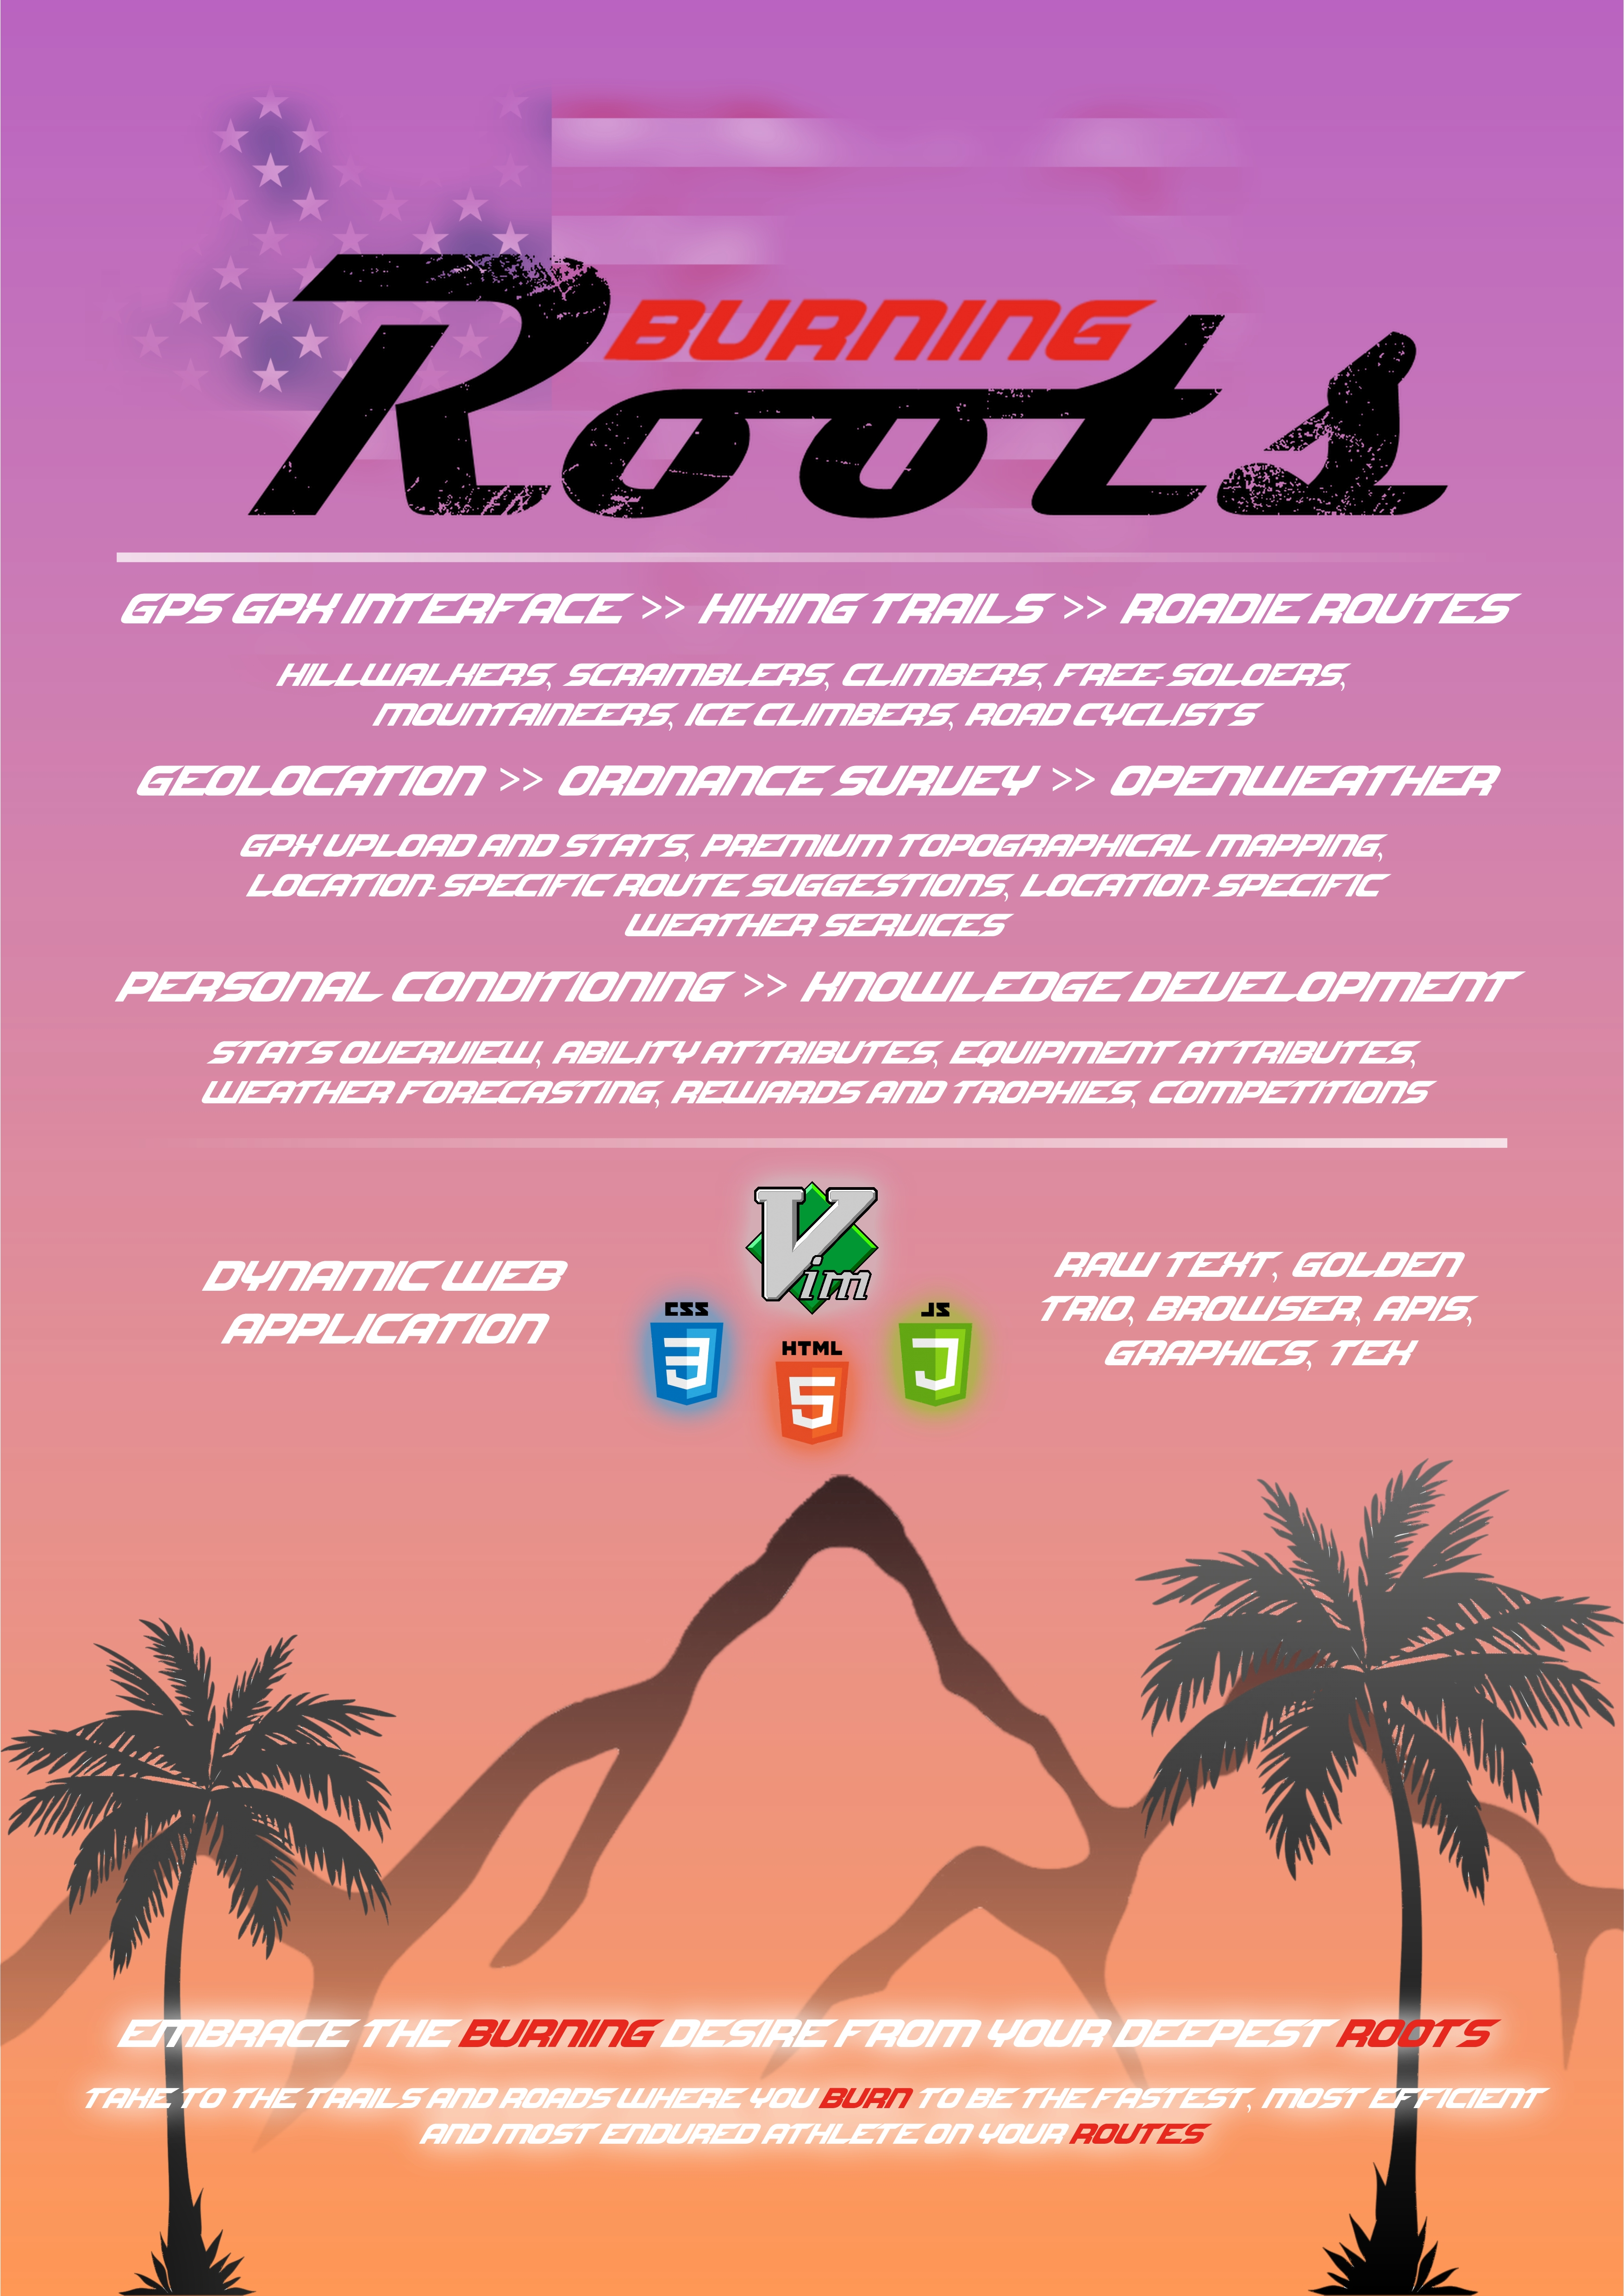
\includegraphics[width=14cm,height=20cm]{poster.jpg}
	\end{center}

\newpage

		\subsubsection*{Figure A6: Functions Summary}

	\begin{center}
		\scriptsize
	\begin{longtable}{p{4cm}p{6cm}p{2cm}}
		\textsc{Inputs} & \textsc{Data/Computation} & \textsc{Return/Out.}\\
		\hline
		\hline
		\multicolumn{3}{c}{\textsc{`Overview'}}\\
		\hline \hline
		\multicolumn{3}{c}{\textsc{Score Route}}\\
		\hline
		\multicolumn{3}{c}{\underline{\texttt{scoreRoute()}}}\\
		Elevation (number), distance (number), number of tops (number), types (array), stages (array), terrain types (array), terrain difficulties (array) & Conversion constant (ft--m), conversion constant (mi--km), types weight, stages weight, terrain types weight, terrain difficulties weight, types element weights, stages element weights, terrain types element weights, terrain difficulties element weights, types values, stages values, terrain types values, terrain difficulties values & Number\\
		\hline
		\multicolumn{3}{c}{\textsc{Describe Route Score}}\\
		\hline
		\multicolumn{3}{c}{\underline{\texttt{describeScore()}}}\\
		Route score (number) & Inequality interval calculation & String\\
		\hline
		\multicolumn{3}{c}{\textsc{Search Route}}\\
		\hline
		\multicolumn{3}{c}{\underline{\texttt{searchRoute()}}}\\
		Landmass name (string) & Route name, route distance, route elevation, route time, route score (\texttt{scoreRoute()}), route difficulty (\texttt{describeRoute()}), route types, route stages, route terrain types, route terrain difficulties, route gear, route Munros, route Munro Tops, route Corbetts, route Corbett Tops, route GPXfile & \texttt{innerHTML}\\
		\hline
		\multicolumn{3}{c}{\textsc{Search Landmass}}\\
		\hline
		\multicolumn{3}{c}{\underline{\texttt{searchLocation()}}}\\
		Landmass name (string) & Landmass name, landmass type, landmass sub-type, landmass sub-sub-type, landmass parent landmass, landmass parent peak, landmass region, landmass sub-region, landmass informal region, hill name, hill type, hill elevation, hill latitude, hill longitude, hill latitude bearing, hill longitude bearing, hill prominence, hill isolation, hill summit feature, hill image & \texttt{innerHTML}\\
		\hline
		\hline
		\multicolumn{3}{c}{\textsc{`Conditioning'}}\\
		\hline
		\hline
		\multicolumn{3}{c}{\textsc{Search `Ability'}}\\
		\hline
		\multicolumn{3}{c}{\underline{\texttt{selectAbility()}}}\\
		Ability component (string) & Ability component name, ability component description, ability component image & \texttt{innerHTML}\\
		\hline
		\multicolumn{3}{c}{\textsc{Search `Equipment'}}\\
		\hline
		\multicolumn{3}{c}{\underline{\texttt{selectEquipment()}}}\\
		Equipment component (string) & Equipment component name, equipment component description, equipment component image, equipment component compatibility, equipment component features, equipment component advantages, equipment component dangers & \texttt{innerHTML}\\
		\hline
		\hline
		\multicolumn{3}{c}{\textsc{`Weather'}}\\
		\hline
		\hline
		\multicolumn{3}{c}{\textsc{Select Munro for Lat/Lon}}\\
		\hline
		\multicolumn{3}{c}{\underline{\texttt{selectMunroOpt()}}}\\
		N/A & Munro latitude, Munro longitude, Munro name & Number [2], \texttt{innerHTML} [2]\\
		\hline
		\multicolumn{3}{c}{\textsc{Input Munro for Lat/Lon}}\\
		\hline
		\multicolumn{3}{c}{\underline{\texttt{inpMunroOpt()}}}\\
		N/A & Munro latitude, Munro longitude, Munro name & Number [2], \texttt{innerHTML} [2]\\
		\hline
		\multicolumn{3}{c}{\textsc{Select Corbett}}\\
		\hline
		\multicolumn{3}{c}{\underline{\texttt{selectCorbettOpt()}}}\\
		N/A & Corbett latitude, Corbett longitude, Corbett name & Number [2], \texttt{innerHTML}\\
		\hline
		\multicolumn{3}{c}{\textsc{Input Corbett}}\\
		\hline
		\multicolumn{3}{c}{\underline{\texttt{inpCorbettOpt()}}}\\
		N/A & Corbett latitude, Corbett longitude, Corbett name & Number [2], \texttt{innerHTML}\\
		\hline
		\multicolumn{3}{c}{\textsc{Select County}}\\
		\hline
		\multicolumn{3}{c}{\underline{\texttt{selectCounty()}}}\\
		N/A & County latitude, County longitude, County name & Number [2], \texttt{innerHTML}\\
		\hline
		\multicolumn{3}{c}{\textsc{Get Weather}}\\
		\hline
		Latitude (number), longitude (number) & Day/time, day weather icon, day weather phrase, day weather description, day max temperature, day minimum temperature, day-day feels-like temperature, day-night feels-like temperature, day precipitation amount, day wind direction, day wind speed, day pressure, day humidity, day dew point, day UV, sunrise, sunset, hour, hour weather icon, hour temperature, hour feels-like temperature, hour precipitation amount, hour wind direction, hour wind speed, hour wind gust, hour pressure, hour humidity, hour dew point, hour visibility, hour UV & \texttt{innerHTML}\\
		\hline
		\hline
		\multicolumn{3}{c}{\textsc{`Conquest Map'}}\\
		\hline
		\hline
		\multicolumn{3}{c}{\textsc{Open Options Menu}}\\
		\hline
		\multicolumn{3}{c}{\underline{\texttt{openOptions()}}}\\
		N/A & N/A & Alter style (\texttt{style.width})\\
		\hline
		\multicolumn{3}{c}{\textsc{Close Options Menu}}\\
		\hline
		\multicolumn{3}{c}{\underline{\texttt{closeOptions()}}}\\
		N/A & N/A & Alter style (\texttt{style.width})\\
		\hline
		\multicolumn{3}{c}{\textsc{Center to Current Location}}\\
		\hline
		\multicolumn{3}{c}{\underline{\texttt{findLocation()}}}\\
		N/A & Accuracy radius (\texttt{accuracy}), Leaflet marker (current coordinates), Leaflet circle (current coordinates) & Leaflet marker\\
		\hline
		\multicolumn{3}{c}{\textsc{Center to Current Location}}\\
		\hline
		\multicolumn{3}{c}{\underline{\texttt{showLocation()}}}\\
		N/A & N/A & (\texttt{map.locate}), Leaflet marker (\texttt{findLocation()})\\
		\hline
		\multicolumn{3}{c}{\textsc{Show Nearest Hill}}\\
		\hline
		\multicolumn{3}{c}{\underline{\texttt{showNearest()}}}\\
		Hill type (string) & Current latitude, Current longitude, Leaflet marker (origin coordinates), Leaflet marker (destination coordinates), distance (\texttt{.distanceTo}), converted distance (km-mi) & \texttt{map.setView}, Leaflet marker (\texttt{createHillMarker()}), \texttt{innerHTML}\\
		\hline
		\multicolumn{3}{c}{\textsc{Show Pan Coordinates}}\\
		\hline
		Move (event) & Center-map coordinates (\texttt{getLatLng()}) & \texttt{innerHTML}\\
		\hline
		\multicolumn{3}{c}{\textsc{Change Map Layer}}\\
		\hline
		\multicolumn{3}{c}{\underline{\texttt{switchLayer()}}}\\
		N/A & Map type & Leaflet layer \texttt{L.titleLayer}\\
		\hline
		\multicolumn{3}{c}{\textsc{Create Hill Marker}}\\
		\hline
		\multicolumn{3}{c}{\underline{\texttt{createHillMarker()}}}\\
		Hill name (string), hill type (string), hill elevation (number), hill latitude (number), hill longitude (number), hill latitude bearing (string), hill longitude bearing (string), hill region (string), hill sub-region (string), hill informal region (string), hill image (string), hill icon type (string) & Popup string, Leaflet marker & Array $+$\\
		\hline
		\multicolumn{3}{c}{\textsc{Create Route Marker}}\\
		\hline
		\multicolumn{3}{c}{\underline{\texttt{createRouteMarker()}}}\\
		Route name (string), route distance (number), route time (number), route score (number), route difficulty (string), route Munros (array), route Munro Tops (array), route Corbetts (array), route Corbett Tops (array), route coordinates (array), route icon type (string) & Popup string, Leaflet marker & Array $+$\\
		\hline
		\multicolumn{3}{c}{\textsc{Show Munros}}\\
		\hline
		\multicolumn{3}{c}{\underline{\texttt{showMunros()}}}\\
		N/A & Hill name, hill elevation, hill latitude, hill longitude, hill latitude bearing, hill longitude bearing, hill region, hill sub-region, hill informal region, hill image & Leaflet marker (\texttt{createHillMarker()})\\
		\hline
		\multicolumn{3}{c}{\textsc{Show Munro Tops}}\\
		\hline
		\multicolumn{3}{c}{\underline{\texttt{showMunroTops()}}}\\
		N/A & Hill name, hill elevation, hill latitude, hill longitude, hill latitude bearing, hill longitude bearing, hill region, hill sub-region, hill informal region, hill image & Leaflet marker (\texttt{createHillMarker()})\\
		\hline
		\multicolumn{3}{c}{\textsc{Show Corbetts}}\\
		\hline
		\multicolumn{3}{c}{\underline{\texttt{showCorbetts()}}}\\
		N/A & Hill name, hill elevation, hill latitude, hill longitude, hill latitude bearing, hill longitude bearing, hill region, hill sub-region, hill informal region, hill image & Leaflet marker (\texttt{createHillMarker()})\\
		\hline
		\multicolumn{3}{c}{\textsc{Show Corbett Tops}}\\
		\hline
		\multicolumn{3}{c}{\underline{\texttt{showCorbettTops()}}}\\
		N/A & Hill name, hill elevation, hill latitude, hill longitude, hill latitude bearing, hill longitude bearing, hill region, hill sub-region, hill informal region, hill image & Leaflet marker (\texttt{createHillMarker()})\\
		\hline
		\multicolumn{3}{c}{\textsc{Show Munro}}\\
		\hline
		\multicolumn{3}{c}{\underline{\texttt{showMunro()}}}\\
		Hill name (string) & Hill name, hill elevation, hill latitude, hill longitude, hill latitude bearing, hill longitude bearing, hill region, hill sub-region, hill informal region, hill image & Leaflet marker (\texttt{createHillMarker()})\\
		\hline
		\multicolumn{3}{c}{\textsc{Show Munro Top}}\\
		\hline
		\multicolumn{3}{c}{\underline{\texttt{showMunroTop()}}}\\
		Hill name (string) & Hill name, hill elevation, hill latitude, hill longitude, hill latitude bearing, hill longitude bearing, hill region, hill sub-region, hill informal region, hill image & Leaflet marker (\texttt{createHillMarker()})\\
		\hline
		\multicolumn{3}{c}{\textsc{Show Corbett}}\\
		\hline
		\multicolumn{3}{c}{\underline{\texttt{showCorbett()}}}\\
		Hill name (string) & Hill name, hill elevation, hill latitude, hill longitude, hill latitude bearing, hill longitude bearing, hill region, hill sub-region, hill informal region, hill image & Leaflet marker (\texttt{createHillMarker()})\\
		\hline
		\multicolumn{3}{c}{\textsc{Show Corbett Top}}\\
		\hline
		\multicolumn{3}{c}{\underline{\texttt{showCorbettTop()}}}\\
		Hill name (string) & Hill name, hill elevation, hill latitude, hill longitude, hill latitude bearing, hill longitude bearing, hill region, hill sub-region, hill informal region, hill image & Leaflet marker (\texttt{createHillMarker()})\\
		\hline
		\multicolumn{3}{c}{\textsc{Hide All Markers}}\\
		\hline
		\multicolumn{3}{c}{\underline{\texttt{hideMarkers()}}}\\
		N/A & Loop array & \texttt{map.removeLayer}\\
		\hline
		\multicolumn{3}{c}{\textsc{Filter Routes by `Ability'}}\\
		\hline
		\multicolumn{3}{c}{\underline{\texttt{selectAbilityRefine()}}}\\
		Ability component (string) & Show and hide elements & \texttt{innerHTML}\\
		\multicolumn{3}{c}{\underline{\texttt{addAbilityRefine()}}}\\
		Ability component (string) & Loop array & Array $+$\\
		\hline
		\multicolumn{3}{c}{\textsc{Filter Routes by `Equipment'}}\\
		\hline
		\multicolumn{3}{c}{\underline{\texttt{addEquipmentRefine()}}}\\
		Ability component (string) & Loop array & Array $+$\\
		\hline
		\multicolumn{3}{c}{\textsc{Search Filtered Route}}\\
		\hline
		\multicolumn{3}{c}{\underline{\texttt{searchRouteRefined()}}}\\
		Landmass name (string) & Route name, route distance, route elevation, route time, route score (\texttt{scoreRoute()}), route difficulty (\texttt{describeRoute()}), route types, route stages, route terrain types, route terrain difficulties, route gear, route Munros, route Munro Tops, route Corbetts, route Corbett Tops, route GPX file & \texttt{innerHTML}\\
		\hline
		\multicolumn{3}{c}{\textsc{Get Distance (Current Location)}}\\
		\hline
		\multicolumn{3}{c}{\underline{\texttt{getLatLon()}}}\\
		Leaflet position (array) & N/A & \texttt{innerHTML} [2]\\
		\hline
		\multicolumn{3}{c}{\textsc{Get Distance (Current Location)}}\\
		\hline
		\multicolumn{3}{c}{\underline{\texttt{getDistanceCurr()}}}\\
		Destination latitude (number), destination longitude (number) & Current latitude, Current longitude, Leaflet marker (current coordinates), Leaflet marker (destination coordinates), distance (\texttt{.distanceTo}), converted distance (km--mi) & Number\\
		\hline
		\multicolumn{3}{c}{\textsc{Get Distance (Custom)}}\\
		\hline
		\multicolumn{3}{c}{\underline{\texttt{getDistance()}}}\\
		Origin latitude (number), origin longitude (number), destination latitude (number), destination longitude (number) & Current latitude, Current longitude, Leaflet marker (origin coordinates), Leaflet marker (destination coordinates), distance (\texttt{.distanceTo}), converted distance (km--mi) & Number\\
		\hline
		\multicolumn{3}{c}{\textsc{Score Route}}\\
		\hline
		\multicolumn{3}{c}{\underline{\texttt{scoreRoute()}}}\\
		Elevation (number), distance (number), number of tops (number), types (array), stages (array), terrain types (array), terrain difficulties (array) & Conversion constant (ft--m), conversion constant (mi--km), types weight, stages weight, terrain types weight, terrain difficulties weight, types element weights, stages element weights, terrain types element weights, terrain difficulties element weights, types values, stages values, terrain types values, terrain difficulties values & Number\\
		\hline
		\multicolumn{3}{c}{\textsc{Describe Route Score}}\\
		\hline
		\multicolumn{3}{c}{\underline{\texttt{describeScore()}}}\\
		Route score (number) & Inequality interval calculation & String\\
		\hline
		\multicolumn{3}{c}{\textsc{Search Route}}\\
		\hline
		\multicolumn{3}{c}{\underline{\texttt{searchRoute()}}}\\
		Landmass name (string) & Route name, route distance, route elevation, route time, route score (\texttt{scoreRoute()}), route difficulty (\texttt{describeRoute()}), route types, route stages, route terrain types, route terrain difficulties, route gear, route Munros, route Munro Tops, route Corbetts, route Corbett Tops, route GPX file & \texttt{innerHTML}\\
		\hline
		\multicolumn{3}{c}{\textsc{Search Refined Route}}\\
		\hline
		\multicolumn{3}{c}{\underline{\texttt{searchRouteRefined()}}}\\
		Landmass name (string) & Route name, route distance, route elevation, route time, route score (\texttt{scoreRoute()}), route difficulty (\texttt{describeRoute()}), route types, route stages, route terrain types, route terrain difficulties, route gear, route Munros, route Munro Tops, route Corbetts, route Corbett Tops, route GPX file & \texttt{innerHTML}\\
		\hline
		\multicolumn{3}{c}{\textsc{Show Route GPX}}\\
		\hline
		\multicolumn{3}{c}{\underline{\texttt{showRoute()}}}\\
		Landmass name (string) & Route name, route distance, route elevation, route time, route score (\texttt{scoreRoute()}), route Munros, route Munro Tops, route Corbetts, route Corbett Tops, GPX file start coordinates & \texttt{map.setView}, Leaflet marker(s) (\texttt{showMunro}, \texttt{showMunroTop}, \texttt{showCorbett}, \texttt{showCorbettTop}), Leaflet marker (\texttt{createRouteMarker()}), Leaflet line\\
		\hline
		\multicolumn{3}{c}{\textsc{Show Refined Route GPX}}\\
		\hline
		\multicolumn{3}{c}{\underline{\texttt{showRouteRefined()}}}\\
		Landmass name (string) & Route name, route distance, route elevation, route time, route score (\texttt{scoreRoute()}), route Munros, route Munro Tops, route Corbetts, route Corbett Tops, GPX file start coordinates & \texttt{map.setView}, Leaflet marker(s) (\texttt{showMunro}, \texttt{showMunroTop}, \texttt{showCorbett}, \texttt{showCorbettTop}), Leaflet marker (\texttt{createRouteMarker()}), Leaflet line\\
		\hline
		\multicolumn{3}{c}{\textsc{Search Landmass}}\\
		\hline
		\multicolumn{3}{c}{\underline{\texttt{searchLocation()}}}\\
		Landmass name (string) & Landmass name, landmass type, landmass sub-type, landmass sub-sub-type, landmass parent landmass, landmass parent peak, landmass region, landmass sub-region, landmass informal region, hill name, hill type, \texttt{hideMarkers()}, \texttt{hideRoutes()}, hill elevation, hill latitude, hill longitude, hill latitude bearing, hill longitude bearing, hill prominence, hill isolation, hill summit feature, hill image, hillMarker (\texttt{createHillMarker()}), hillFromTo (\texttt{getDistanceCurr}) & \texttt{innerHTML}, \texttt{map.setView}\\
		\hline
		\multicolumn{3}{c}{\textsc{Show All Routes (Galactic Conquest)}}\\
		\hline
		\multicolumn{3}{c}{\underline{\texttt{galacticConquest()}}}\\
		Landmass name (string) & Route name, route distance, route elevation, route time, route score (\texttt{scoreRoute()}), route Munros, route Munro Tops, route Corbetts, route Corbett Tops, GPX file start coordinates & Leaflet marker(s) (\texttt{showMunro}, \texttt{showMunroTop}, \texttt{showCorbett}, \texttt{showCorbettTop}), Leaflet marker (\texttt{createRouteMarker()}), Leaflet line, \texttt{alert}\\
		\hline
		\multicolumn{3}{c}{\textsc{Hide All Routes}}\\
		\hline
		\multicolumn{3}{c}{\underline{\texttt{hideRoutes()}}}\\
		N/A & Loop array & \texttt{map.removeLayer}\\
		\hline
		\multicolumn{3}{p{14cm}}{Note that some functions, such as ones which simply show elements etc., are omitted here. Repeating functions also only appear once.}\\
		\hline
		\caption{Functions Summary}
	\end{longtable}
	\end{center}

\newpage

		\subsubsection*{Figure A7: Functionality -- Continuous Testing (Heuristic Evaluation)}

	\begin{center}
                \scriptsize
        \begin{longtable}{p{7.5cm}p{0.5cm}p{0.5cm}p{4cm}}
                \textsc{Description} & \textsc{Vio.} & \textsc{Sev.} & \textsc{Proposed Solution}\\
                \hline
		\hline
		\multicolumn{4}{c}{\textsc{Functionality}}\\
		\hline
		\hline
		\multicolumn{4}{c}{\textsc{Page Select -- `Drafting Room' and `Conquest Map'}}\\
		\hline
		\textbf{Pages Drop Element}:\newline Seems unnecessary to use a drop-down element to display only one working page (`Conquest Map') under `Field' when the other (`Ranger') is simply a string of text with no link. & $\mathrm{H_{3}}$, $\mathrm{H_{4}}$, $\mathrm{H_{8}}$ & $\mathrm{S_{2}}$ & Remove drop-down element and replace drop-down link `Field' with a simple page link to the `Conquest Map', named `Conquest'; like `Drafting'\\
		\textbf{Summary Section}:\newline The `Quick Burn' summary section on the home page has very little purpose and serves minimal beneficial function to users as it only returns two sets of semi-contextualized text. It seems out of place and unfitting with the subsequent quality of elements & $\mathrm{H_{2}}$, $\mathrm{H_{4}}$, $\mathrm{H_{7}}$ & $\mathrm{S_{2}}$ & Remove HTML elements and all associated functions. Functions appear later in more `functional' contexts later anyway\\
		\textbf{Weather Result Title}:\newline Two functions exist when requesting weather results from the `Weather' section: one which feeds the relevant coordinates values into the `Latitude' and `Longitude' input boxes, and one which requests weather results form the API using those values. It can be confusing when the user either selects a location for the first time or selects another location while results for one are already displayed, and the results don't appear/change due to the requirement to trigger the second function with a button & $\mathrm{H_{4}}$, $\mathrm{H_{7}}$ & $\mathrm{S_{2}}$ & Add ellipsis (...) suffix to the title displayed upon function executed by the selection of a location and remove the suffix upon function executed when the button is selected to fetch results. Therefore, implying ``waiting for interaction'', ``not waiting for interaction''\\
		\textbf{Map Layer Select}:\newline Map layer select options were originally contained within the pop-out options menu. This was not optimally intuitive as users would often overlook it when browsing more advanced functions. For those who did use it, the portion of the viewable map remaining with the menu expanded was not ideal for sampling and choosing different map layers when cycling through them & $\mathrm{H_{3}}$, $\mathrm{H_{7}}$ & $\mathrm{S_{2}}$ & Give the map layer options their own element on the equivalent level of the options menu toggle. Thus seeing that everything in the options menu layers upon the map, and everything outwith the options menu changes the map itself. It also opens the entire map space for sampling layers\\
		\textbf{Show Corbett Tops}:\newline Show Munros, Show Munro Tops, Show Corbetts and Show Corbett Tops all operate fine upon initial inspection however, if Show Corbett Tops is toggled then a route is shown, the Leaflet line displaying the GPX coordinates does not scale to map zoom. I.e. it remains the same relative size to the initial level of zoom. If just the latter three `show' options have been toggled, this issue does not occur. & $\mathrm{H_{4}}$, $\mathrm{H_{5}}$ & $\mathrm{S_{2}}$ & Many-an-hour have been exerted on this issue but I'm afraid I give up. I'm not spending any more time on it. I am [Pink Wojak] (Figure B4).\\
		\textbf{Show Nearest Munro/Corbett}:\newline Both of these buttons (using the same function) work fine when used in isolation however, when using the function to show the nearest Munro after using it to show the nearest Corbett, no values are returned. Contrastingly, when using the function to show the nearest Corbett after using it to show the nearest Munro, there are no issues. & $\mathrm{H_{4}}$, $\mathrm{H_{5}}$ & $\mathrm{S_{2}}$ & Many-an-hour have been exerted on this issue but I'm afraid I give up. I'm not spending any more time on it. I am [Pink Wojak] (Figure B4).\\
		\textbf{Search Route}:\newline Displaying a summary and the route (on map) of a route all at once feels slightly ``cluttered'' as an HTML element is being filled with a significant amount of text while the center of the map is finding the start of a route and printing multiple pieces on it. These two functions also produce their results at different speeds, adding a slightly ``cheap'' delayed feel to the process & $\mathrm{H_{3}}$, $\mathrm{H_{4}}$, $\mathrm{H_{7}}$ & $\mathrm{S_{2}}$ & Separate the functions into two of their own features which are executed through two separate options. That is, a user can view a summary of a route before deciding if they wish to print it, with its attributes, on the map\\
		\textbf{Route Display Error}:\newline When displaying some routes on the `Conquest Map', the part of the function used to return the start coordinates, and thus place a Leaflet marker and center the map to there, returns a value which cannot be translated using the coordinate conversion algorithm. Therefore, when these routes are selected the map is centered somewhere completely irrelevant; in the middle of the ocean & $\mathrm{H_{5}}$ & $\mathrm{S_{3}}$ & Unfortunately, no immediate solution as this is an issue based on the structure of particular GPX files. This occurs purely with GPX files downloaded from Walkhighlands' official source; not with walk report (user donated) GPX files or with my own. Given more time, non-official-Walkhighlands replacements for these files would be found, however, the functionality is still clearly there and can be executed upon all other GPX files\\
		\hline
		\hline
		\multicolumn{4}{c}{\textsc{Design \& Accessibility}}\\
		\hline
		\hline
		\multicolumn{4}{c}{\textsc{Header \& Footer -- `Drafting Room' and `Conquest Map'}}\\
		\hline
		\textbf{Header Contrast}:\newline There isn't enough contrast between the black logo and the header background color however, there is almost too much contrast between the navigation font color and the header background color & $\mathrm{H_{8}}$ & $\mathrm{S_{2}}$ & Experiment with gradients to balance the contrast. This will also add a themes of speed and urgency, and harmonise with the directional transition of the logo upon page load\\
		\textbf{Background Image}:\newline The background image arguably contains [1] too many cold colors and [2] too much variation in geometry and layers, meaning it's complexity takes-away from the content intended to primarily be used by the user & $\mathrm{H_{4}}$ $\mathrm{H_{7}}$, $\mathrm{H_{8}}$ & $\mathrm{S_{2}}$ & Replace image with one which integrates more appropriate warm colors which are relevant to the context and consistent geometry and layers which make content easily viewable\\
		\textbf{Logo Drop Shadow}:\newline With the new warm-colored, basic-layered background image, the black and red logo becomes slightly less easily visible & $\mathrm{H_{8}}$ & $\mathrm{S_{2}}$ & Add a deeper drop shadow to the logo to add contrast between it and the background image\\
		\textbf{Button Hover Color-Transparency Ratio}:\newline The `Begin Conquest' button on the intro section always has an opacity value which is less then 1. When `hovered' upon, the background of the button fills with a transparent white to match the border. The opacity value is too low to make the text easily visible on the white background & $\mathrm{H_{8}}$ & $\mathrm{S_{2}}$ & Either [1] Increase the opacity value of the button's colors, or [2] change the white hover background color to something which doesn't lose as much dominance when made slightly transparent. Option 2 executed\\
		\textbf{Intro Text}:\newline The large body of introductory text on the intro background image appears in a fully opaque white. Due to the length of the text, the repetitive white text take the form of white lines which take-away from the other elements in the section & $\mathrm{H_{8}}$ & $\mathrm{S_{2}}$ & Experiment with opacity values of the text color to find the correct balance of readability and harmony with the background\\
		\textbf{`Briefing' Titles and Symbols}:\newline The three selectable headings in the `Briefing' section were originally presented just using their associated FontAwesome symbols to attempt to keep this process minimal. However, although the symbols are relevant, they only become clearly so after viewing each section and therefore, remove form the efficiency they were intended to create & $\mathrm{H_{4}}$, $\mathrm{H_{7}}$, $\mathrm{H_{8}}$ & $\mathrm{S_{2}}$ & Add relevant heading text to indicate sections\\
		\textbf{Options Menu}:\newline The options menu for the `Conquest Map' requires a significant amount of space due to its capabilities therefore, making a large portion of the map not-viewable when it's expanded. This cannot be directly altered however may require some additional design feature to make the menu blend-in a bit more naturally & $\mathrm{H_{4}}$, $\mathrm{H_{8}}$ & $\mathrm{S_{2}}$ & Add slight transparency to the background of the options menu to make other portions of the page and map viewable while it's expanded, and add a layer of depth as opposed to being faced with a box of white space over a pretty map\\
		\textbf{`Seeking' Bar}:\newline The seeking bar displaying two empty value fields adds a ``cheap'' feel to the map before the user pans to display the panning coordinates & $\mathrm{H_{4}}$, $\mathrm{H_{7}}$ & $\mathrm{S_{2}}$ & Hide the `Seeking' bar until the user has begun panning the map\\
		\hline
                \multicolumn{4}{l}{\textsc{Total Violations}: 16}\\
                \multicolumn{4}{l}{\textsc{Total Iterations}: 11}\\
		\multicolumn{4}{l}{\textsc{Iteration Frequency}: Appropriate Checkpoints}\\
		\multicolumn{4}{l}{\textsc{Evaluator(s)}: Lewis Britton, Anonymous [5]}\\
                \multicolumn{4}{l}{\textsc{Platform(s)}: Brave Browser (Desktop), Brave Browser (Mobile)}\\
                \hline
                \caption{Functionality -- Continuous Testing (Heuristic Evaluation)}
        \end{longtable}
        \end{center}

\newpage

		\subsubsection*{Figure A8: Functionality -- Isolated/Comprehensive Testing}

	\begin{center}
		\scriptsize
	\begin{longtable}{p{3cm}p{8cm}p{2cm}}
		\textsc{Element} & \textsc{Expected} & \textsc{Actual}\\
		\hline
		\hline
		\multicolumn{3}{c}{\textsc{Functionality}}\\
		\hline
		\hline
		\multicolumn{3}{c}{\textsc{Page Select -- `Drafting Room' and `Conquest Map')}}\\
		\hline
		\texttt{href} (link) & Navigate to `Drafting Room' page & As expected\\
		\texttt{href} (link) & Navigate to `Conquest Map' page & As expected\\
		\texttt{href} (button) & Navigate to `Conquest Map' page & As expected\\
		\hline
		\multicolumn{3}{c}{\textsc{Page Select -- `Drafting Room' and `Conquest Map') (Mobile)}}\\
		\hline
		\texttt{EventListener} (click) & Display page-select drop-down division & As expected\\
		\texttt{href} (link) & Navigate to `Drafting Room' page & As expected\\
		\texttt{href} (link) & Navigate to `Conquest Map' page & As expected\\
		\texttt{href} (button) & Navigate to `Conquest Map' page & As expected\\
		\hline
		\multicolumn{3}{c}{\textsc{`Drafting Room' -- Intro}}\\
		\hline
		\multicolumn{3}{c}{\underline{\texttt{getLocation()}}}\\
		\texttt{function} (button),\newline \texttt{alert} & Display browser-specific request to use device's location, and display device coordinates & As expected\\
		\multicolumn{3}{c}{\underline{\texttt{showNearest()}}}\\
		\texttt{function} (button) & Display nearest hill to device & As expected, minor issue noted in Figure A7\\
		\hline
		\multicolumn{3}{c}{\textsc{`Drafting Room' -- `Briefing'}}\\
		\hline
		\texttt{EventListener} (link) & Display `Overview' division & As expected\\
		\texttt{EventListener} (link) & Display `Conditioning' division & As expected\\
		\texttt{EventListener} (link) & Display `Weather' division & As expected\\
		\hline
		\multicolumn{3}{c}{\textsc{`Drafting Room' -- `Briefing' -- `Overview'}}\\
		\hline
		\multicolumn{3}{c}{\underline{\texttt{showRouteListCont()}}}\\
		\texttt{function} (select) & Display division of relevant landmass selection\newline (18 variations) & As expected\\
		\texttt{option} (select) & Select route on landmass selection\newline (Varying between 1 and 7 variations, for 18 parent variations) & As expected\\
		\multicolumn{3}{c}{\underline{\texttt{searchRoute(`<route>')}}}\\
		\texttt{function} (button) & Display division of relevant selection$^{1}$ & As expected\\
		\texttt{text} (input) & Accept input relevant to any hill name & As expected\\
		\multicolumn{3}{c}{\underline{\texttt{searchLocation()}}}\\
		\texttt{function} (button) & Display division of relevant input match$^{2}$ & As expected\\
		\hline
		\multicolumn{3}{c}{\textsc{`Drafting Room' -- `Briefing' -- `Conditioning'}}\\
		\hline
		\multicolumn{3}{c}{\underline{\texttt{showAbilityListCont()}}}\\
		\texttt{function} (select) & Display division of relevant ability selection\newline (7 variations) & As expected\\
		\multicolumn{3}{c}{\underline{\texttt{selectAbility(`<ability>')}}}\\
		\texttt{function} (select) & Select ability factor on ability selection, and display division of relevant selection\newline (Varying between 4 and 22 \texttt{<ability>} variations, for 7 parent variations$^{3}$) & As expected\\
		\multicolumn{3}{c}{\underline{\texttt{showEquipmentListCont()}}}\\
		\texttt{function} (select) & Display division of relevant equipment selection\newline (4 variations) & As expected\\
		\multicolumn{3}{c}{\underline{\texttt{selectEquipment(`<equip>')}}}\\
		\texttt{function} (select) & Select equipment factor on equipment selection, and display division of relevant selection\newline (Varying between 11 and 24 \texttt{<equip>} variations, for 4 parent variations$^{4}$) & As expected\\
		\hline
		\multicolumn{3}{c}{\textsc{`Drafting Room' -- `Briefing' -- `Weather'}}\\
		\hline
		\multicolumn{3}{c}{\underline{\texttt{selectMunroOpt()}}}\\
		\texttt{function} (select) & Select Munro, and populate latitude and longitude fields\newline (25 variations) & As expected\\
		\multicolumn{3}{c}{\underline{\texttt{inpMunroOpt()}}}\\
		\texttt{function} (input) & Accept input relevant to any Munro name, and populate latitude and longitude fields & As expected\\
		\multicolumn{3}{c}{\underline{\texttt{selectCorbettOpt()}}}\\
		\texttt{function} (select) & Select Corbett, and populate latitude and longitude fields\newline (11 variations) & As expected\\
		\multicolumn{3}{c}{\underline{\texttt{inpCorbettOpt()}}}\\
		\texttt{function} (input) & Accept input relevant to any Corbett name, and populate latitude and longitude fields & As expected\\
		\multicolumn{3}{c}{\underline{\texttt{selectCounty()}}}\\
		\texttt{function} (select) & Select region, and populate latitude and longitude fields\newline (33 variations) & As expected\\
		\texttt{text} (input) & Accept latitude input & As expected\\
		\texttt{text} (input) & Accept longitude input & As expected\\
		\multicolumn{3}{c}{\underline{\texttt{getLocation}}}\\
		\texttt{EventListener} (click),\newline \texttt{alert} & Display browser-specific request to use device's location, and populate latitude and longitude fields with device coordinates$^{1}$ & As expected\\
		\multicolumn{3}{c}{\underline{\texttt{fetchWeather}}}\\
		\texttt{EventListener} (click) & Display daily and hourly weather data for coordinates$^{5}$ & As expected\\
		\texttt{EventListener} (link) & Display `Key' division & As expected\\
		\texttt{EventListener} (link) & Display `Suggested Reading on Cloud Types' division & As expected\\
		\texttt{EventListener} (link) & Display `Suggested Reading on Bearings' division & As expected\\
		\hline
		\multicolumn{3}{c}{\textsc{`Conquest Map' -- Accept Device Location}}\\
		\hline
		\multicolumn{3}{c}{\underline{\texttt{getCurrentPosition( getLatLon, getLatLonFail, getLatLonOpts)}}}\\
		\texttt{alert} & Display browser-specific request to use device's location & As expected\\
		\hline
		\multicolumn{3}{c}{\textsc{`Conquest Map' -- Display Pan Coordinates}}\\
		\hline
		\texttt{EventListener} (move) & Display crosshair at center of map & As expected\\
		\hline
		\multicolumn{3}{c}{\textsc{`Conquest Map' -- Display Pan Coordinates}}\\
		\hline
		\texttt{EventListener} (move) & Display center pan coordinates of map in HTML element & As expected\\
		\hline
		\multicolumn{3}{c}{\textsc{`Conquest Map' -- Cycle Map Layers}}\\
		\hline
		\multicolumn{3}{c}{\underline{\texttt{switchLayer()}}}\\
		\texttt{radio} (input) & Change OS map layer\newline (3 variations) & As expected\\
		\hline
		\multicolumn{3}{c}{\textsc{`Conquest Map' -- Toggle Options Menu}}\\
		\hline
		\multicolumn{3}{c}{\underline{\texttt{openOptions()}}}\\
		\texttt{function} (link) & Display HTML element containing more options, with transition & As expected\\
		\multicolumn{3}{c}{\underline{\texttt{closeOptions()}}}\\
		\texttt{function} (link) & Hide HTML element containing more options, with transition & As expected\\
		\hline
		\multicolumn{3}{c}{\textsc{`Conquest Map' -- Location Options}}\\
		\hline
		\multicolumn{3}{c}{\underline{\texttt{showLocation()}}}\\
		\texttt{function} (button),\newline \texttt{alert} & Display browser-specific request to use device's location, pan to device coordinates on map, display marker and associated pop-up, and display accuracy radius & As expected\\
		\multicolumn{3}{c}{\underline{\texttt{showNearest(`<hill>')}}}\\
		\texttt{function} (button),\newline \texttt{alert} & Display browser-specific request to use device's location, use hill type parameter to determine whether the hill is a Munro or Corbett, pan to nearest hill coordinates on map, display marker and associated pop-up, and display relevant HTML element & As expected\\
		\hline
		\multicolumn{3}{c}{\textsc{`Conquest Map' -- Feature Options}}\\
		\hline
		\multicolumn{3}{c}{\underline{\texttt{showMunros()}}}\\
		\texttt{function} (button) & Display all markers and associated pop-ups of Munros & As expected\\
		\multicolumn{3}{c}{\underline{\texttt{showMunroTops()}}}\\
		\texttt{function} (button) & Display all markers and associated pop-ups of Munro Tops & As expected\\
		\multicolumn{3}{c}{\underline{\texttt{showCorbetts()}}}\\
		\texttt{function} (button) & Display all markers and associated pop-ups of Corbetts & As expected\\
		\multicolumn{3}{c}{\underline{\texttt{showCorbettTops()}}}\\
		\texttt{function} (button) & Display all markers and associated pop-ups of Corbett Tops & As expected\\
		\multicolumn{3}{c}{\underline{\texttt{hideMarkers()}}}\\
		\texttt{function} (button) & Hide all markers associated with any hill$^{A}$ & As expected\\
		\hline
		\multicolumn{3}{c}{\textsc{`Conquest Map' -- `Ability' Options}}\\
		\hline
		\multicolumn{3}{c}{\underline{\texttt{showAbilityListCont()}}}\\
		\texttt{function} (select) & Display division of relevant ability selection\newline (7 variations) & As expected\\
		\multicolumn{3}{c}{\underline{\texttt{selectAbilityRefine(`<ability>')}}}\\
		\texttt{function} (select) & Display child divisions of relevant ability selection\newline (3 variations)\\
		\multicolumn{3}{c}{\underline{\texttt{addAbilityRefine(`<ability>')}}}\\
		\texttt{function} (button) & Select ability factor on ability selection, add ability factor to list, and display in HTML element & As expected\\
		\hline
		\multicolumn{3}{c}{\textsc{`Conquest Map' -- `Equipment' Options}}\\
		\hline
		\multicolumn{3}{c}{\underline{\texttt{showEquipmentListCont()}}}\\
		\texttt{function} (select) & Display division of relevant equipment selection\newline (7 variations) & As expected\\
		\multicolumn{3}{c}{\underline{\texttt{addEquipmentRefine(`<equip>')}}}\\
		\texttt{function} (button) & Select equipment factor on equipment selection, add equipment factor to list, and display in HTML element & As expected\\
		\hline
		\multicolumn{3}{c}{\textsc{`Conquest Map' -- Search Route}}\\
		\hline
		\multicolumn{3}{c}{\underline{\texttt{showRouteListCont()}}}\\
		\texttt{function} (select) & Display division of relevant landmass selection\newline (18 variations) & As expected\\
		\texttt{option} (select) & Select route on landmass selection\newline (Varying between 1 and 7 variations, for 18 parent variations) & As expected\\
		\multicolumn{3}{c}{\underline{\texttt{searchRoute(`<route>')}}}\\
		\texttt{function} (button) & Display division of relevant selection$^{6}$ & As expected\\
		\multicolumn{3}{c}{\underline{\texttt{showRoute(`<route>')}}}\\
		\texttt{function} (button) & Pan to route coordinates on map, display marker and associated pop-up, display line, and display hill markers and associated pop-ups & As expected\\
		\multicolumn{3}{c}{\underline{\texttt{searchRouteRefined(`<route>')}}}\\
		\texttt{function} (button) & Display division of relevant selection$^{7}$\newline (Subject to `Ability' and `Equipment' constraints) & As expected\\
		\multicolumn{3}{c}{\underline{\texttt{showRouteRefined(`<route>')}}}\\
		\texttt{function} (button) & Pan to route coordinates on map, display marker and associated pop-up, display line, and display hill markers and associated pop-ups\newline (Subject to `Ability' and `Equipment' constraints) & As expected\\
		\multicolumn{3}{c}{\underline{\texttt{hideRoutes()}}}\\
		\texttt{function} (button) & Hide all route components associated with any route & As expected\\
		\multicolumn{3}{c}{\underline{\texttt{galacticConquest()}}}\\
		\texttt{function} (button) & Display all markers and associated pop-ups, display all lines, and display all hill markers and associated pop-ups$^{B}$ & As expected\\
		\hline
		\multicolumn{3}{c}{\textsc{`Conquest Map' -- Search Landmass}}\\
		\hline
		\texttt{text} (input) & Accept input relevant to any hill name & As expected\\
		\multicolumn{3}{c}{\underline{\texttt{searchLocation()}}}\\
		\texttt{function} (button) & Display division of relevant input match$^{2}$ & As expected\\
		\hline
		\hline
		\multicolumn{3}{c}{\textsc{Design \& Accessibility}}\\
		\hline
		\hline
		\multicolumn{3}{c}{\textsc{Header \& Footer -- `Drafting Room' and `Conquest Map'}}\\
		\hline
		\texttt{header}, \texttt{body} & Logo font is easily readable & As expected\\
		\texttt{header}, \texttt{body} & Logo font color is easily readable & As expected\\
		\texttt{header} & Logo transitions entry from left to right, then parks & As expected\\
		\texttt{header} & Navigation font is easily readable & As expected\\
		\texttt{header} & Navigation font color is easily readable & As expected\\
		\texttt{header} & Navigation (\texttt{a}) font color changes to a blue with transition upon hover & As expected\\
		\texttt{header} & Navigation (\texttt{a}) hover font color is easily readable & As expected\\
		\texttt{header}, \texttt{body} & Linear gradient creates a sufficient contrast for dark logo font and lighter navigation font & As expected\\
		\texttt{body} & Credits font is easily readable & As expected\\
		\texttt{body} & Credits font color is easily readable & As expected\\
		\hline
		\multicolumn{3}{c}{\textsc{Body Elements -- `Drafting Room' and `Conquest Map'}}\\
		\hline
		\texttt{h1}, \texttt{h2}, \texttt{h3}, \texttt{p}, \texttt{b}, \texttt{i} & Heading (and variant), paragraph, bold-face, and italic fonts are easily readable & As expected\\
		\texttt{h1}, \texttt{h2}, \texttt{h3}, \texttt{p}, \texttt{b}, \texttt{i}, \texttt{small} & Heading (and variant), paragraph, bold-face, italic and `small' font sizes are easily readable & As expected\\
		\texttt{body} & There is sufficient contrast between the black body text and white (and variants) background and foregrounds & As expected\\
		\texttt{body} & Margins and padding between parent and child division elements is sufficient enough to create an effective and readable partition & As expected\\
		\texttt{a} & Link font color changes to a blue upon hover, unless otherwise specified & As expected\\
		\texttt{a} & Link hover font color is easily readable & As expected\\
		\texttt{button} & Button font reverse (white on graded grey) provides sufficient contrast & As expected\\
		\texttt{button} & Buttons remain readable with the size reduction upon click & As expected\\
		\texttt{select} & Select font reverse (white on graded grey) provides sufficient contrast & As expected\\
		\texttt{input} & Input font reverse (white on graded grey) provides sufficient contrast & As expected\\
		\texttt{a}, \texttt{button}, \texttt{select}, \texttt{input} & Links, buttons, selects and input all provide a `pointer' cursor upon hover & As expected\\
		\texttt{head} & All FontAwesome symbols load where expected, to the best of knowledge & As expected\\
		\texttt{head} & All FontAwesome symbols are appropriate and would make relevant indications if used in isolation & As expected\\
		\hline
		\multicolumn{3}{c}{\textsc{Introduction -- `Drafting Room'}}\\
		\hline
		\texttt{body} & There is sufficient contrast between the varying logo and body text, and background picture & As expected\\
		\texttt{img} & Background image remains fixed upon scroll & As expected\\
		\texttt{img} & Main logo can be seen with drop-shadow over background image & As expected\\
		\texttt{button} & Button background color changes to a blue upon hover & As expected\\
		\texttt{button} & Button reduces in opacity upon hover & As expected\\
		\texttt{button} & Button is easily readable with reduced opacity upon hover & As expected\\
		\texttt{marquee} & Marquee scrolls right-to-left & As expected\\
		\texttt{p} & Body text is easily readable with reduced opacity & As expected\\
		\hline
		\multicolumn{3}{c}{\textsc{`Briefing' (`Overview', `Conditioning' and `Weather') -- `Drafting Room'}}\\
		\hline
		\texttt{body}, \texttt{p} & There is sufficient contrast between the black symbols and the light-blue gradient of the `Briefing' navigation elements & As expected\\
		\texttt{body}, \texttt{p} & There is sufficient contrast between the body text and the light-blue gradient of the `Search Route' and `Search Landmass' results & As expected\\
		\texttt{img} & Result images are an appropriate size to be easily viewable on `Search Landmass', `Ability' and `Equipment' & As expected\\
		\texttt{body} & Margins and padding between parent and child division elements in `Weather' result tiles is sufficient enough to create an effective and readable partition & As expected\\
		\multicolumn{3}{c}{\underline{\texttt{selectMunroOpt()}, \texttt{selectCorbettOpt()}, \texttt{selectCounty()}}}\\
		\texttt{span}$^{X}$, \texttt{function} (select) & Ellipses appear succeeding ``Five day forecast for'' and ``Seven hour forecast for'' to indicate a `Weather' location's coordinates have been primed but not yet used to return results & As expected\\
		\multicolumn{3}{c}{\underline{\texttt{showWeather}}}\\
		\texttt{function} (click) & Ellipses succeeding ``Five day forecast for'' and ``Seven hour forecast for'' disappear when `Get Weather' is selected, executing the primary function, to indicate a `Weather' location's coordinates have now been used to return results & As expected\\
		API \texttt{function} & `Weather' daily and hourly respective dates and hours are correct, to the best of knowledge & As expected\\
		\multicolumn{3}{c}{\underline{showWeather}}\\
		\texttt{function} (click) & `Weather' summary symbols match descriptions and other stats such as precipitation & As expected\\
		\multicolumn{3}{c}{\underline{showWeather}}\\
		\texttt{function} (click) & `Weather' temperature background colors change relative to temperature intervals & As expected\\
		\multicolumn{3}{c}{\underline{showWeather}}\\
		\texttt{function} (click) & `Weather' temperature FontAwesome symbol colors change relative to temperature intervals (temperature background colors) & As expected\\
		\multicolumn{3}{c}{\underline{showWeather}}\\
		\texttt{function} (click) & `Weather' wind direction statistics are aligned. For example, a `SW' wind will have an arrow pointing approximately 45\textdegree\ and read something like ``$x$m/s \@ 225\textdegree'' & As expected\\
		\texttt{table} & Table font is easily readable in `Exclusive DLC' & As expected\\
		\texttt{table} & Table images are an appropriate size to be easily viewable `exclusive DLC' & As expected\\
		\hline
		\multicolumn{3}{c}{\textsc{Toggles -- `Conquest Map'}}\\
		\hline
		\texttt{header}, \texttt{body} & Proportion of header, `seeking bar', options toggle, and map layer select are relatively appropriate to the map to still create a viewable map division & As expected\\
		\texttt{body} & Double right angle delimiters ($\rangle\rangle$) are an appropriate method of suggesting clicking `this' generates some form of left-to-right movement (the extension of the options menu) & As expected\\
		\texttt{input} & Only one `Leisure', `Road', `Outdoor' is selected at one time & As expected\\
		\texttt{input} & `Leisure', `Road', and `Outdoor' are not only selectable by clicking in the \texttt{input} \texttt{radio}s, but also by clicking on the words themselves & As expected\\
		\hline
		\multicolumn{3}{c}{\textsc{Options Menu -- `Conquest Map'}}\\
		\hline
		\multicolumn{3}{c}{\underline{\texttt{openOptions()}}}\\
		\texttt{function} & Element transitions from left-to-right when toggled active & As expected\\
		\multicolumn{3}{c}{\underline{\texttt{closeOptions()}}}\\
		\texttt{function} & Element transitions from right-to-left when toggled inactive & As expected\\
		\texttt{body} & When active, proportion of the options menu is relatively appropriate to the map to create a viewable map division on which toggling options can be viewed to a reasonable degree & As expected\\
		\texttt{body} & Reduced opacity background is sufficient enough to make it's text easily readable but add depth to the element & As expected\\
		\texttt{body} & Margins and padding between parent and child division elements is sufficient enough to create an effective and readable partition & As expected\\
		\texttt{img} & Result images are an appropriate size to be easily viewable on `Search Landmass' & As expected\\
		\texttt{button} & Different-styled buttons are still recognisable as buttons & As expected\\
		\texttt{button} & Button font and border color changes to a blue upon hover, unless otherwise specified & As expected\\
		\texttt{button} & Button hover font and border color is easily readable & As expected\\
		\hline
		\multicolumn{3}{c}{\textsc{Map Layers -- `Conquest Map'}}\\
		\hline
		\texttt{body} & `Seeking bar' does not display upon map load & As expected\\
		\texttt{body} & `Seeking bar' reduced opacity background is sufficient enough to make it's text easily readable but add depth to the element & As expected\\
		API \texttt{function} & Map pans effectively using cursor control & As expected\\
		API \texttt{function} & Map layers alternate between OS Road (1 : 250 000), OS Landranger (1 : 50 000), and OS Explorer (1 : 25 000) accordingly upon zoom, in-line with the OS API & As expected\\
		\texttt{body} & Markers (FontAwesome hill for hills, FontAwesome map pin for start of route, FontAwesome arrow for current location) are all relevant and easily viewable on the map base layer & As expected\\
		\texttt{body} & Red route lines are easily viewable on the map base layer & As expected\\
		API \texttt{function} & Clicking on an appropriate marker toggles it's pop-up active & As expected\\
		Leaflet \texttt{bindPopup} & Clicking on the `$\times$' on a marker's pop-up toggles the pop-up inactive & As expected\\
		\texttt{body} & White pop-ups on markers provide enough contrast to the map base layer to be easily readable & As expected\\
		\texttt{p} & Font of pop-ups on markers is easily readable & As expected\\
		\texttt{img} & Images on pop-ups on markers are an appropriate size to be easily viewable & As expected\\
		\hline
		\multicolumn{3}{c}{\textsc{Mobile Scalability -- `Drafting Room' and `Conquest Map')}}\\
		\hline
		\texttt{header} & `Drafting' and `Conquest' on navigation are replaced by the click-prompting `hamburger bars' & As expected\\
		\texttt{body} & The footer becomes hidden & As expected\\
		\texttt{body} & Margins and padding between parent and child division elements is sufficient enough upon change to still create an effective and readable partition & As expected\\
		\texttt{header}, \texttt{body} & Proportion of header, `seeking' bar, options toggle, and map layer select are still relatively appropriate to the map to still create a viewable map division & As expected\\
		\texttt{body} & Home introduction section is replaced with a similar one, contained within a foreground container, with black replacing white as the color of the \texttt{button} and \texttt{marquee} & As expected\\
		\texttt{div} & `Briefing' navigation elements stack in three rows, rather than one & As expected\\
		\texttt{body} & Margins and padding between parent and child division elements in `Weather' result tiles is still sufficient enough to create an effective and readable partition upon scale & As expected\\
		\texttt{div} & `Weather' daily and hourly tile elements stack in five and seven rows, respectively; rather than one and one by five and seven, respectively & As expected\\
		\texttt{table} & Table font is still easily readable in `exclusive DLC' upon scale & As expected\\
		\texttt{table} & Table images are still an appropriate size to be easily viewable `exclusive DLC' upon scale & As expected\\
		API \texttt{function} & `Conquest Map' map pans effectively using finger control & As expected\\
		\texttt{body} & When active, proportion of the `Conquest Map' options menu populates the majority of the map division, not a percentage-proportionate (to desktop site) portion & As expected\\
		\hline
		\multicolumn{3}{p{12.5cm}}{$N$ Evaluator(s): 5\newline Iterations (Isolated): 2 /element/evaluator\newline Iterations (Comprehensive): 3 /evaluator\newline $^{1,2,3,4,5,6,7}$: Clients informed of expected HTML output\newline $^{A,B}$: ``all'' refers to ``for all hills'' and ``for all routes'', respectively\newline $^{X}$: Ellipses appear in span text, in HTML however are also added back using a function after a different function removes them}\\
		\hline
		\caption{Functionality -- Isolated/Comprehensive Testing}
	\end{longtable}
	\end{center}

\newpage

	\subsection*{Appendix 2: Foundational Material}

		\subsubsection*{Figure B1: Linguistics of `{\LaTeX}'}

		{\LaTeX} (or LaTeX, even latex (Donald E. Knuth's more recent installment of {\TeX})) is usually pronounced /la\textlengthmark t$\varepsilon$k/ (`lah') or /le\textsc{i}t$\varepsilon$k/ (`lei'/`lay') in English (that is, not with the /ks/ pronunciation English speakers normally associate with X, but with a /k/). The characters T, E, X in the name come from capital Greek letters tau, epsilon, and chi, as the name of {\TeX} derives from the Greek: $\tau\varepsilon\chi\nu\eta$ (skill, art, technique, precision); for this reason, Donald E. Knuth promotes a pronunciation of /t$\varepsilon$k/ (tekh) (that is, with a voiceless velar fricative as in Modern Greek, similar to the last sound of the German word ``Bach", the Spanish ``j" sound, or as ``ch'' in a Scottish `loch'). 

		%F\"{u}hrer
		\subsubsection*{Figure B2: Don. Knuth's Computer Modern Unicode (CMU) Font Family}

		\begin{table}[h]
			\scriptsize
			\renewcommand{\arraystretch}{1.25}
		\begin{center}
		\begin{tabular}{p{4cm}p{4cm}p{4cm}}
			\hline
			\multicolumn{1}{c}{\textbf{Serif}} & \multicolumn{1}{c}{\textbf{Sans Serif}} & \multicolumn{1}{c}{\textbf{Monospaced}}\\
			\hline
			CMU Serif Roman & \textsf{CMU Sans Serif} & \texttt{CMU Concrete}\\
			\textbf{CMU Serif Bold} & \sffamily \textbf{CMU Sans Serif Bold} & \\ 
				\textit{CMU Serif Italic} & & \ttfamily \textit{CMU Concrete Italic}\\
			\textsl{CMU Serif Oblique} & \sffamily \textsl{CMU Sans Serif Oblique} & \ttfamily \textsl{CMU Concrete Oblique}\\
				\textsc{CMU Serif Small Caps} & & \ttfamily \textsc{CMU Concrete Small Caps}\\
			\hline
				\multicolumn{3}{p{13cm}}{\textit{In the presence of traditionalists, a suitable alternative to Donald E. Knuth's Computer Modern Unicode font family may be considered: Andale Mono.}}\\
			\hline
		\end{tabular}
		\end{center}
		\end{table}

\newpage

		\subsubsection*{Figure B3: Lorn and Lorne}

		Many of the uneducated among us (hahaha) often confuse the term `Lorn' with `Lorne'. Although it's argued by many inbred highlanders that the two words may be used interchangeably, our slavemasters at Ordnance Survey have determined otherwise; that `Lorn' refers to the division found in the OS region \textit{Fort William, Lochaber and Lorn} (as printed in OS Explorer 384: Glen Coe \& Glen Etive); where, `Lorne' refers to the popular breakfast food choice of alcoholics, drug addicts, and fine gentlemen named Derek.\\

		Henceforth, when in the region of Fort William, Lochaber and Lorn, myself and my gentlemen often like to retire after a long night at [BAR] to [Lee's kitchen] where we will cook up a storm of Lorne. Over many hours of experimentation and trials, we have produced the following rankings:

		\begin{table}[h]
			\scriptsize
			\renewcommand{\arraystretch}{1.25}
		\begin{center}
		\begin{tabular}{rr|p{1.25cm}p{3.5cm}p{2.5cm}}
			\textsc{\#} & \textsc{Brand} & \textsc{Beef \%} & \textsc{Description} & \textsc{Photograph}\\
			\hline
			1 & House of Bruar & 78\% & A rich, almost gamey, flavour with a tender flesh and effective distribution of seasoning. Not quite the H.o.B. discontinued (R.I.P.) venison Lorne though. & \vspace{-0.25cm}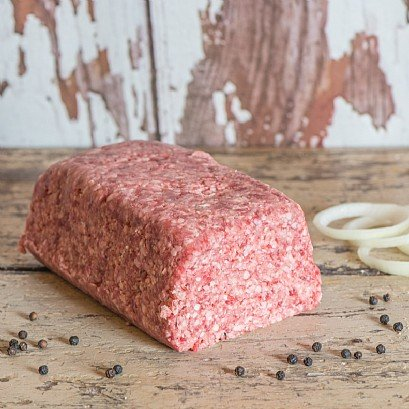
\includegraphics[width=2.5cm]{bruar_lorne.jpg}\\
			2 & Simon Howie (Steak) & \textasciitilde40\% & A rough but tender texture and very traditionally `meaty' flavour. Proper steak that. & \vspace{-0.25cm}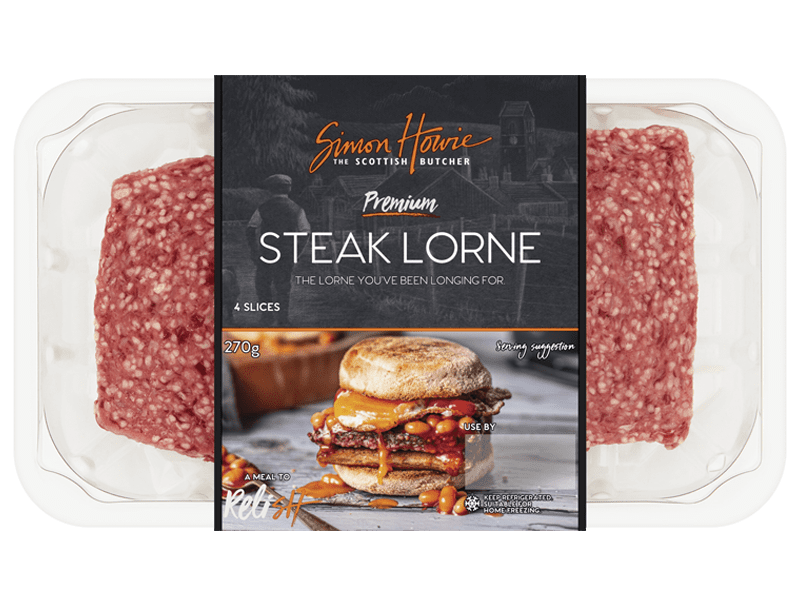
\includegraphics[width=2.5cm]{sh_lorne.png}\\
			3 & Marks \& Spencer & \textasciitilde40\% & Very similar to Mr. Howie's however a little more fatty on occasion and sometimes under-seasoned. For some reason better when part of the M\&S breakfast pack. & \vspace{-0.25cm}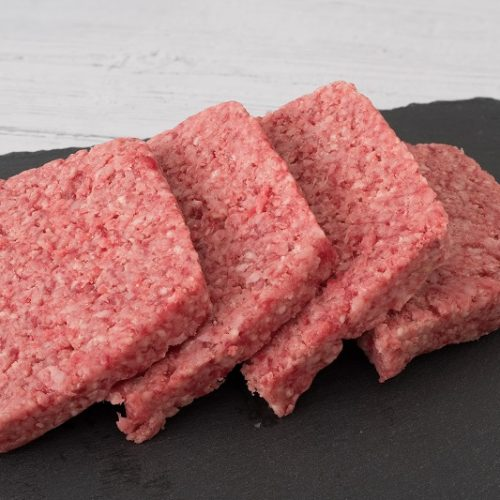
\includegraphics[width=2.5cm]{ms_lorne.jpeg}\\
			4 & Simon Howie (Beef) & \textasciitilde35\% & Slightly underwhelming and rubbery version of the steak pieces, with a less meaty flavour, bordering on the fatty side. & \vspace{-0.25cm}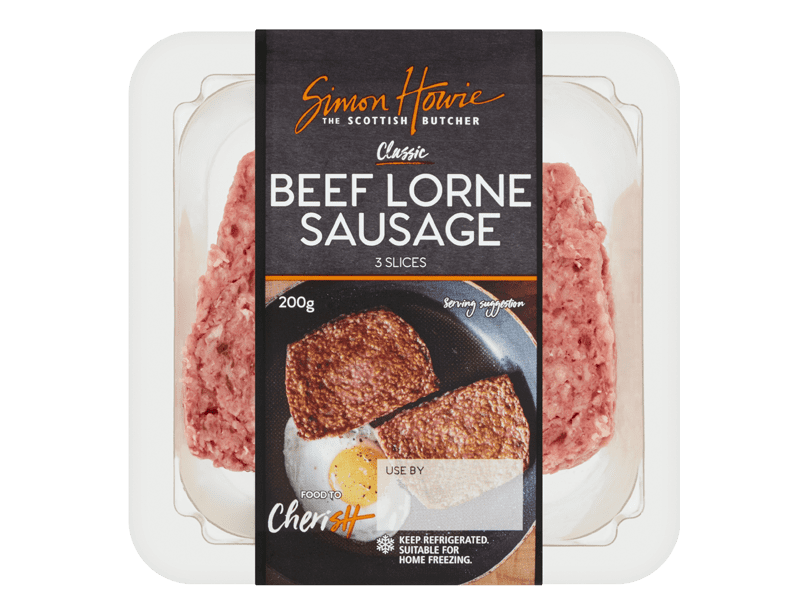
\includegraphics[width=2.5cm]{sh_lorne2.png}\\
			5 & Malcolm Allan & \textasciitilde30\% & Hockey puck of grease. Not much more to be said. Alright in Aviemore as long as Ross isn't in charge with the deep fried in butter beta. & \vspace{-0.25cm}
\includegraphics[width=2.5cm]{ma_lorne.jpg}\\
			\hline
		\end{tabular}
			\caption{Lorne Rankings}
		\end{center}
		\end{table}

\newpage

		\subsubsection*{Figure B4: Pink Wojak}
	
	\begin{center}	
		\verb|find ~/memes| $\mathtt{\vert}$ \verb|grep -i pink| $\mathtt{\vert}$ \verb|shuf| $\mathtt{\vert}$ \verb|sxiv -ia|\\[2cm]
		
\includegraphics[width=14cm,height=14cm]{pink.png}
	\end{center}

\newpage

	\renewcommand\refname{Bibliography}

	\fancyhead[L]{\leftmark}

	\begin{thebibliography}{9}

	\bibitem{}
		Chart.js. (2022).
		\textsl{Chart.js.}
		Available At:
		\texttt{https://www.chartjs.org/docs/latest/}
		(Accessed: 03/04/2022).

	\bibitem{}
		Elastic. (2022).
		\textsl{Elastic Stack: Elasticsearch, Kibana, Beats.}
		Available At:
		\texttt{https://www.elastic.co/elastic-stack/}
		(Accessed: 22/07/2022).

	\bibitem{}
		FontAwesome. (2021).
		\textsl{Search v5 Icons | Font Awesome.}
		Available At:
		\texttt{https://fontawesome.com/v5/search}
		(Accessed: 08/04/2022).

	\bibitem{}
		Harold Street. (2022).
		\textsl{Mountain GPS Waypoints \& Hill Bagging Lists.}
		Available At:
		\texttt{https://www.haroldstreet.org.uk/waypoints/}
		(Accessed: 03/04/2022).

	\bibitem{}
		Knuth, D. E. (2020).
		\textsl{Computer Musings.}
		Available At:
		\texttt{https://www-cs-faculty.stanford.edu/knuth/musings.html.}
		(Accessed 21/07/2022).

	\bibitem{}
		Leaflet. (2022).
		\textsl{Documentation - Leaflet - a JavaScript library for interactive maps.}
		Available At:
		\texttt{https://leafletjs.com/reference-1.7.1.html}
		(Accessed: 03/04/2022).

	\bibitem{}
		Mapbox. (2022).
		\textsl{toGeoJSON.}
		Available At:
		\texttt{https://mapbox.github.io/togeojs on/}
		(Accessed: 03/04/2022).

	\bibitem{}
		MDN Web Docs. (2022).
		\textsl{Geolocation API - MDN Web Docs.}
		Available At:
		\texttt{https://developer.mozilla.org/en-US/docs/Web/API/Geolocation\_API}
		(Accessed: 08/04/2022).

	\bibitem{}
		Moolenaar, B. (2020).
		\textsl{Bram Moolenaar's Website - home.}
		Available At:
		\texttt{https://moolenaar.net.}
		(Accessed 21/07/2022).

	\bibitem{}
		Nielsen, J. (1994).
		\textsl{Heuristic Evaluation.}
		Usability Inspection Methods, John Wiley \& Sons

	\bibitem{}
		OpenWeather. (2022).
		\textsl{One Call API: weather data for any geographical coordinate - OpenWeatherMap.}
		Available At:
		\texttt{https://openweathermap.org/api/one-call-api}
		(Accessed: 03/04/2022).

	\bibitem{}
		Ordnance Survey. (2022).
		\textsl{Examples | OS Data Hub.}
		Available At:
		\texttt{https://labs.os.uk/public/os-data-hub-exam ples/os-names-api/find-example-placename}
		(Accessed: 03/04/2022).

	\bibitem{}
		Peakbagger.com (2022).
		\textsl{Search - Peakbagger.com.}
		Available At:
		\texttt{https://www.peakbagger.com/Search.aspx}
		(Accessed: 03/04/2022).

	\bibitem{}
		Smith, L. (2015).
		\textsl{External Possession and the Undisentanglability of Syntax and Semantics.}
		University of Georgia.

	\bibitem{}
		US3699296A. (1972).
		\textsl{Catastrophically Buckling Compression Column Switch and Actuator.}
		International Business Machines Corporation.

	\bibitem{}
		Vim Diesel. (2020).
		\textsl{Luke Smith's Website.}
		Available At:
		\texttt{https://lukesmith.xyz.}
		(Accessed 21/07/2022).

	\bibitem{}
		Walkhighlands. (2022).
		\textsl{Walkhighlands: Scotland walks and accommodation.}
		Available At:
		\texttt{https://www.walkhighlands.co.uk/}
		(Accessed: 22/03/2022).

	\end{thebibliography}

\end{document}
